%\stepcounter{contsubsec} 
\section{INTRODUCCIÓN}

La determinación y el control de actitud en satélites son esenciales para el éxito de una misión espacial. Existen diferentes métodos de control de actitud, los cuales pueden clasificarse como pasivos y activos. El control pasivo recurre principalmente al diseño geométrico y magnético del satélite, buscando aprovechar los principios físicos y fuerzas naturales que actúan sobre el satélite, aumentando los efectos de una mientras se minimizan los de otras. Por otro lado, el control activo emplea actuadores como propulsores, magnetorquers (barra de torsión) o ruedas de reacción (Reaction Wheels, RW)  para modificar la actitud del satélite mediante la generación de torques correctivos \cite{Wertz1999}. Durante una misión espacial, se pueden utilizar diferentes modos de control de actitud para sus diferentes fases y tareas del satélite.
En los últimos años, se ha presentado un aumento de misiones espaciales que involucran CubeSats, el cual es un tipo de nanosatélite formado a partir de unidades cúbicas (U) de 10 cm de lado, y que cada vez presentan una mayor complejidad. Por lo tanto, ha sido de gran interés el incremento de la vida útil y el rendimiento de las misiones, donde el sistema de determinación y control de actitud (Attitude Determination and Control System, ADCS)  juegan un papel fundamental para garantizar la probabilidad de éxito \cite{Venturini2018}. En este sentido, el control de actitud de un CubeSat es fundamental para cumplir el perfil de misión, normalmente situado en órbita baja (Low Earth Orbit, LEO),  donde se busca tener precisión de apuntamiento y estabilidad para las cargas útiles, antenas y paneles solares, que son componentes críticos para el funcionamiento de la nave espacial y del éxito de la misión.
El control de actitud en CubeSats es normalmente provisto por RW, las cuales intercambian momento con la nave sin consumir propelente. No obstante, una desventaja de este tipo de dispositivos electromecánicos es que acumulan el momento para mantener una actitud deseada y, en consecuencia, las RW se saturan cuando alcanzan su velocidad máxima de rotación lo cual impiden que estas puedan intercambiar momentos que garanticen a la estabilidad del satélite. Por tal motivo, surge un desafío en el área de control de actitud que busca la desaturación de dichas ruedas de reacción mientras se conserva la actitud del satélite.
Algunos de los desafíos que se presentan frente a este fenómeno se deben a que comúnmente el control de actitud y la desaturación de RW son tratados por separado, y a pesar de que existen numerosos estudios sobre el control de actitud con torques magnéticos, hay pocos artículos que involucran la desaturación del momento de las RW mediante magnetorquers \cite{Yang2017}. Por otro lado, se requieren controladores que garanticen la estabilidad del satélite anticipando y actuando ante perturbaciones presentes en el ambiente espacial como por ejemplo torques externos debido a gradientes gravitacionales, torques aerodinámicos o torques de radiación solar \cite{Kaplan1976}.
Debido a esto, es de particular interés estudiar técnicas de desaturación con controladores, que permitan asistir estos dispositivos recurriendo a otros actuadores auxiliares como los magnetorques, los cuales, por medio de su interacción con campos magnéticos, generan un par que desatura las ruedas de reacción. No obstante, a diferencia de las RW que pueden generar un torque en cualquier dirección y en cualquier momento, los magnetorques dependen de la interacción con el plano ortogonal del campo geomagnético instantáneo, el cual cambia a medida que el satélite orbita alrededor de la tierra \cite{Tregouet2015}. Adicionalmente, a pesar de que los magnetorques son dispositivos confiables en LEO, producen una respuesta más lenta en comparación con otros actuadores lo cual reduce la capacidad de maniobra del satélite y su tiempo de reacción ante perturbaciones externas.
En este sentido, se propone evaluar estrategias de control de actitud que incorporen la desaturación de las ruedas reacción, mediante simulaciones computacionales a partir de un modelo dinámico basado en el CubeSat de entrenamiento EyasSat \cite{Eyassat}. Adicionalmente, se pretende realizar una comparación de diferentes controladores bajo algunos escenarios o perfiles de misión propuestos, con el fin de determinar las condiciones donde mejor se desempeñan las estrategias de control propuestas. La elección de este modelo en particular de CubeSat se debe a que dicho satélite se encuentra disponible en el programa de Ingeniería Aeroespacial; y es de especial interés incluirlo en el planteamiento de las simulaciones porque puede ser aprovechado junto con otros equipos, como la Jaula de Helmholtz, para consolidar una futura línea de investigación en control satelital.


\newpage
%--------------------------------------------

%Las \section{} que para esta plantilla son los títulos de nivel 1 siempre inician en una página nueva. Las \subsection{} y demas particiones de niveles 2 al 4 pueden ir en medio de una página.

\section{PLANTEAMIENTO DEL PROBLEMA}

%Se refiere al interrogante que lleva al investigador a buscar respuestas concretas. Es la definición del problema que aborda con la investigación. 

El fenómeno de desaturación de ruedas de reacción será abordado en un picosatélite tipo CubeSat \textbf{(Fig. \ref{fig:diagrama_problema})}, particularmente en el modelo EyasSat, el cual está equipado con:

\begin{itemize}

\item Una rueda de reacción en el eje Z, por lo que se tendrá control unicamente en un grado de libertad. En este actuador es donde se presenta el fenómeno de estudio, ya que a pesar de proporcionar una respuesta rápida en el control de actitud, sufre de un incremento gradual de su tasa de giro. Lo anterior, debido a su incapacidad para alterar el momento angular total del satélite en presencia de perturbaciones externas. 
 
\item Magnetorquers en el eje X e Y respectivamente, los cuales pueden ejercer torques en los 3 ejes debido a la interacción del campo magnético terrestre. No obstante, el modelo estará restringido a contemplar solo los torques generados en el eje Z con el fin de disminuir la velocidad de rotación que pueda presentar la rueda de reacción. 

\end{itemize}

De esta manera, el problema tratado en este trabajo consiste en el diseño de estrategias de control que permitan eliminar la saturación de ruedas de reacción mediante los magnetorquers, que sirven como actuadores secundarios en el sistema de control de actitud. Dichos dispositivos, deberán garantizar que el momento angular de las ruedas de reacción sea igual momento angular del satélite, evitando una acumulación progresiva de la velocidad de rotación de las RW.
Ya que el rendimiento de los magnetorquers depende de su interacción con el campo geomagnético, es de interés evaluar 3 inclinaciones de órbitas circulares que permitan identificar el escenario mas favorable donde se podrían desempeñar.

Ademas de eliminar el exceso de momento angular, dichas estrategias de desaturación, simultáneamente deben permitir que el satélite alcance una actitud deseada en el marco de referencia del cuerpo ante diferentes respuestas:
\begin{itemize}
	\item Fase de \textit{Detumbling}. 
	\item Respuesta tipo escalón de un angulo deseado.
	\item Respuesta tipo rampa para alcanzar una velocidad de rotación constante.
\end{itemize} 
 

\begin{figure}[!ht]
	\begin{center}
		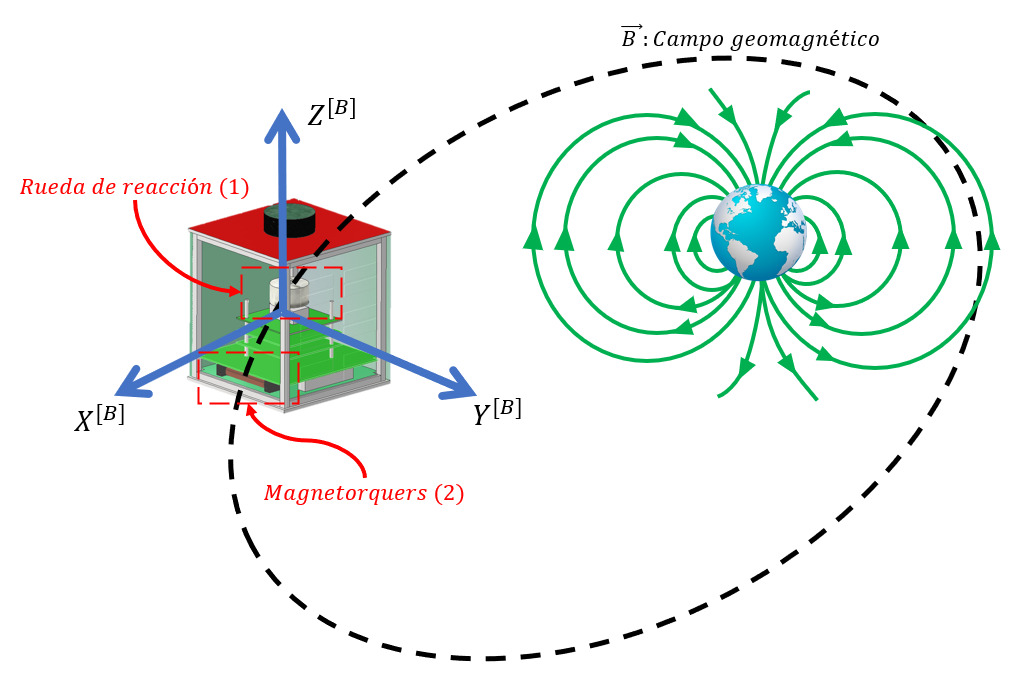
\includegraphics[scale=0.5]{imagenes/planteamiento_del_problema/esquema_planteamiento.PNG}\\
	\end{center}
	\caption{CubeSat EyasSat equipado con 1 rueda de reacción y 2 magnetorquers.}
	\label{fig:diagrama_problema}
%	\footnotesize{Nota. Fuente \url{https://www.ieee.org/}.} %\citep{lib:apa}.
\end{figure}

\section{ESTADO DEL ARTE}

La desaturación de ruedas de reacción es un problema común en los satélites, incluidos los Cubesats, que pueden llevar a una pérdida de control de actitud. La ley de producto cruzado es una solución clásica en ingeniería comúnmente utilizado para resolver este paradigma desde una aproximación lineal \cite{Tregouet2015}. Pero en los últimos años se han desarrollado diferentes controladores que involucran sistemas no lineales.
Sin embargo, tal como se expresa en \cite{Yang2017}, el problema de control de actitud y la saturación de ruedas de reacción es comúnmente abordado como temas separados desde el punto de vista de diseño, por lo cual, no existen tantos artículos en los que se incluyan ambos objetivos. En su trabajo se propone un método de diseño de un LQR periódico variable en el tiempo donde se incluyen los torques generados por gradientes gravitacionales y los efectos periódicos del campo geomagnético alrededor de la órbita. Además, señala que los artículos existentes no suelen estos efectos mencionados anteriormente.
Por otro lado, Yang menciona esfuerzos como el de \cite{Tregouet2015} , en el cual se estudió al mismo tiempo el problema de la estabilización y el de desaturación de ruedas de reacción. A su vez se consideró la variación temporal del campo magnético en el marco del cuerpo (BRF), y su marco de referencia era el marco inercial (ECI). Sin embargo, para una nave espacial en LEO que utiliza el campo geomagnético, el marco de referencia más idóneo es el marco local vertical local horizontal (LVLH). Además, su diseño se compone de dos bucles, que es esencialmente una idea de tratar con el control de actitud y la desaturación en consideraciones separadas.
En esa misma línea, de Angelis \cite{Angelis2016} propuso un controlador proporcional heurístico y utilizó una función de Lyapunov para probar que el controlador puede simultáneamente estabilizar la nave espacial con respecto al marco LVLH y lograr la desaturación de ruedas de reacción. Pero este método de diseño no tiene en cuenta el efecto variable en el tiempo del campo geomagnético en el marco del cuerpo.
Finalmente, al estudiar las estrategias de control ya implementadas y conocer, tanto los efectos que incluyen como las simplificaciones de sus sistemas, es necesario recurrir a un modelo dinámico del EyasSat, el cual es el punto de partida para diseñar los controladores que se evaluarán bajo las condiciones de saturación y de estabilidad. A pesar de, no encontrar modelos dinámicos específicos para el EyasSat, Groenewald y Steyn \cite{Groenewald2014} elaboraron una propuesta para un nuevo ADCS integrado en este cubesat, y en él se incluyen propiedades inerciales y dimensiones útiles para la formulación de un modelo dinámico.
A su vez, en \cite{tes:Sorolla2019} se realiza un desarrollo matemático de la dinámica de un cubesat de 1U, donde describe los diferentes torques y perturbaciones externas, modela los actuadores en Simulink y sus diferentes configuraciones para ser evaluados bajo diferentes condiciones como la desaturación de ruedas de reacción.


\newpage
%-------------------------------


\section{JUSTIFICACIÓN}

 
%Responde a los interrogantes del por qué se desea conocer el tema y por qué se seleccionó, así como cuál es el aporte que tendrá el texto a la ciencia. 
%
%No abuse del uso de \textit{cursivas} o \textbf{negritas} dentro del texto, úselas muy moderadamente, por lo general saturan y dificultan la lectura del documento. Utilice cursivas en casos muy particulares como géneros y especies (\textit{Tyrannus melancholicus}), términos químicos (\textit{kr}), letras griegas ($\beta$) y algunos títulos y subtítulos. El entorno matemático de \LaTeX \ muestra las variables y símbolos en letra cursiva, asegurese de hacer lo mismo al referenciarla en el documento, Utilice \textbf{negritas} en algunos títulos de capítulos y subcapítulos, algunos datos de tablas o enfatizar aspectos muy particulares. El uso de \underline{texto subrayado} no se recomienda en normas IEEE.
%
%Utilice moderadamente el uso de abreviaturas, se prefiere que el texto sea más largo y claro que corto y confuso para el lector. Por ejemplo, IEEE puede significar Institute of Electrical and Electronics Engineers o Instituto Español de Estudios Estratégicos. Sin embargo, las abreviaturas pueden ser útiles en casos como la repetición continua en un mismo párrafo.
%
%Prefiera las comillas “inglesas” y ‘sencillas’ por sobre las «latinas» o «españolas».

Dentro del proceso de diseño de una misión espacial, es fundamental evaluar el rendimiento de los subsistemas de un vehículo con el fin de garantizar el cumplimiento del perfil de misión. Especialmente, en el sector espacial es de vital importancia limitar el consumo de potencia eléctrica para maximizar la vida útil del misión. En este sentido, las técnicas de desaturación de ruedas de reacción, ademas de garantizar la estabilidad y el control de actitud, permiten establecer un balance entre el rendimiento y el consumo de potencia eléctrica al tratar de minimizar la acción de control de los actuadores sin afectar la estabilidad del sistema.

Por otro lado, conocer el desempeño de los magnetorquers según su órbita, permite tener un criterio a la hora de evaluar perfiles de misión que cumplan con los requerimientos y a su vez sean eficientes en materia de consumo de potencia. 

Finalmente, el diseño teórico de controladores crea la oportunidad de evaluarlos en un ambiente controlado, donde se puedan implementar las estrategias de control en sistemas ADCS reales. Para ello, se pretende fomentar una linea de investigación en sistemas de control de actitud, donde se cuenta con una Jaula de Helmholtz  \textbf{(Fig. \ref{fig:jaula})} funcional y operativa, como parte del inventario del grupo de investigación ASTRA de la Universidad de Antioquia. 

\begin{figure}[!ht]
	\begin{center}
		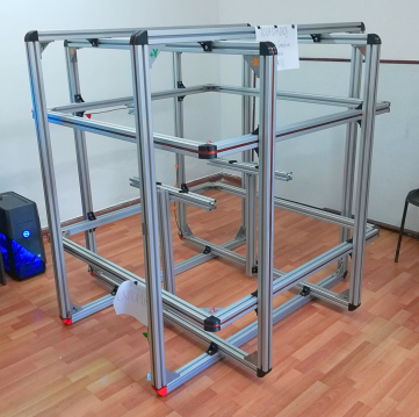
\includegraphics[scale=0.65]{imagenes/justificacion/jaula.PNG}\\
	\end{center}
	\caption{Ensamble Jaula de Helmholtz.}
	\label{fig:jaula}
	%	\footnotesize{Nota. Fuente \url{https://www.ieee.org/}.} %\citep{lib:apa}.
\end{figure}

%\begin{description}
%    \item[Características:] texto descriptivo.
%    \item[Propiedades:] texto descriptivo.
%    \item[Estructura:] texto descriptivo.
%\end{description}

\newpage
%--------------------------
\section{OBJETIVOS}

\subsection{Objetivo general}



%El objetivo general y los objetivos específicos describen lo que se pretende con la investigación, cuál es el alcance y cuál es el problema que se desea resolver. Deben iniciarse con verbos que describan claramente lo que se lleva a cabo.
Validar computacionalmente una estrategia de control de actitud para el picosatélite CubeSat EyasSat que integre la desaturación de sus ruedas de reacción mediante magnetorquers a partir de su modelo dinámico.

\subsection{Objetivos específicos}

%Se describen algunos ejemplos de verbos comunes que se utilizan en el planteamiento de objetivos, los cuales cambiarán dependiendo de su investigación.
\begin{itemize}
\item Simular el comportamiento dinámico del nanosatélite EyasSat a partir del desarrollo de un modelo fenomenológico de este.
\item Determinar una estrategia de control de actitud para el nanosatélite EyasSat que integre la desaturación de las ruedas de reacción empleando magnetorquers a partir de simulaciones computacionales basadas en su modelo dinámico. 
\item Identificar aquellas órbitas donde la estrategia de control presente el mejor desempeño al utilizar los magnetorquers como elementos de desaturación de las ruedas de reacción.

\end{itemize}


\newpage
%--------------------------
%\section{PROBLEMA DE INVESTIGACIÓN}
%
%El problema de investigación es el enunciado de lo que puede ser demostrado o encontrado, y de lo cual se requieren pruebas y evidencias.        

\newpage
%--------------------------
\section{MARCO TEÓRICO}

\subsection{CubeSat y EyasSat}
El concepto CubeSat se refiere a un nanosatélite estándar cuyo diseño fue propuesto por los profesores Jordi Puig-Suari, de la Universidad Politécnica Estatal de California, y Bob Twiggs, de la Universidad de Stanford en 1999. Corresponde a un pequeño satélite constituido por unidades (U) con forma de cubo de 10 cm y una masa de hasta 1.3 kilogramos \cite{Lan2013}. Son ampliamente utilizados alrededor el mundo por universidades ya que representan una alternativa para desplegar cargas científicas en el espacio con un presupuesto inferior a los 100.000 dólares \cite{opc:Satcatalog}. 
No obstante, también son diseñados con fines educativos para que los estudiantes se familiaricen con los principales sistemas que componen estos vehículos espaciales y puedan hacer pruebas de integración y rendimiento en un aula de clase. En este sentido, surge el CubeSat EyasSat \cite{Barnhart2005} como parte de un programa de entrenamiento del Departamento de Astronáutica de la Academia de las Fuerzas Aéreas de Estados Unidos (USAFA). El EyasSat \textbf{(Fig. \ref{fig:eyassat})}, se centra en seis subsistemas de los que constan la mayoría de los satélites. Estos subsistemas son: estructuras, potencia, comunicación y tratamiento de datos, control y determinación de actitud (ADCS), propulsión y sistemas térmicos. No obstante, el diseño modular del EyasSat permite la integración y mejora de subsistemas adicionales que pueden ampliar sus capacidades. Por ejemplo, \cite{Groenewald2014} propone una nueva versión del ADCS, sistema de particular interés en esta investigación, el cual se extiende a tres ejes y permite la capacidad de ser probado en un cojinete de aire.


\begin{figure}[!ht]
	\begin{center}
		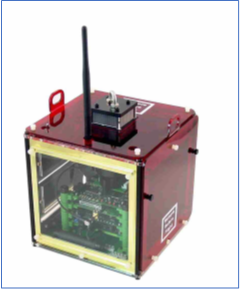
\includegraphics[scale=0.9]{imagenes/marco_teorico/eyassat.PNG}\\
	\end{center}
	\caption{CubeSat de entrenamiento EyasSat.}
	\label{fig:eyassat}
	%	\footnotesize{Nota. Fuente \url{https://www.ieee.org/}.} %\citep{lib:apa}.
\end{figure}

\subsection{Sistema de determinación y control de actitud (ADCS)}

Este sistema se encarga de estabilizar y orientar el vehículo en las direcciones deseadas durante la misión a pesar de los torques de perturbaciones externos que actúan sobre él. Para ello es necesario que el vehículo determine su actitud mediante sensores, y la controle, mediante actuadores.

\begin{figure}[!ht]
	\begin{center}
		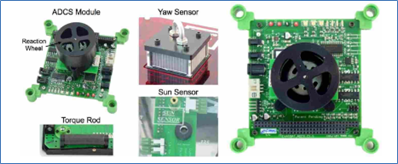
\includegraphics[scale=0.9]{imagenes/marco_teorico/adcs.PNG}\\
	\end{center}
	\caption{ADCS EyasSat.}
	\label{fig:adcs}
	%	\footnotesize{Nota. Fuente \url{https://www.ieee.org/}.} %\citep{lib:apa}.
\end{figure}

El Módulo ADCS del EyasSat \textbf{(Fig. \ref{fig:adcs})}, se compone de dos tipos de actuadores: una rueda de reacción en el eje Z y dos magnetorquers en el eje X e Y respectivamente. En la \textbf{Fig. \ref{fig:eyassat_axes}} se evidencian los ejes coordenados en el marco del cuerpo.
Por otro lado, la medición de la posición se realiza mediante dos sensores solares (situados en la parte superior e inferior del EyasSat) y un sensor solar diferencial-posicional (compuesto por dos células fotovoltaicas) \cite{Ritchey2004}. En este sentido, es posible realizar pruebas de actitud recurriendo a un control de lazo cerrado de un grado de libertad. 

\begin{figure}[!ht]
	\begin{center}
		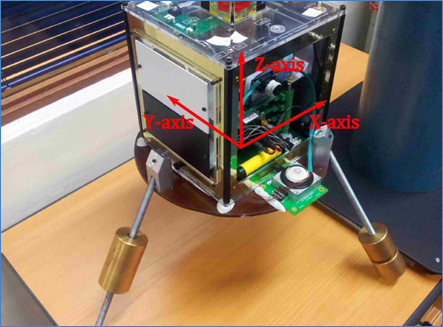
\includegraphics[scale=0.9]{imagenes/marco_teorico/eyassat_axes.PNG}\\
	\end{center}
	\caption{ Ejes coordenados del EyasSat}
	\label{fig:eyassat_axes}
	\footnotesize{Nota. Fuente \cite{Groenewald2014}}
\end{figure}


\subsubsection{Ruedas de reacción}

Las ruedas de reacción (RW) son motores de alto torque acoplados a rotores de gran inercia. Permiten reposicionar vehículos espaciales y satélites controlables mientras están en órbita ya que contienen energía rotacional, almacenada mediante la conservación del momento angular, y pueden activar el intercambio de momento para proporcionar estabilidad a una nave espacial o al satélite.


\begin{figure}[!ht]
	\begin{center}
		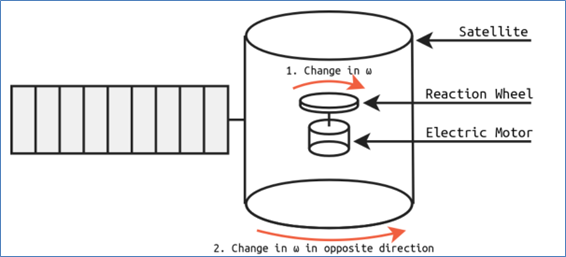
\includegraphics[scale=0.9]{imagenes/marco_teorico/rw.PNG}\\
	\end{center}
	\caption{ Efecto de RW en la velocidad $\omega$ de un satélite.}
	\label{fig:rw_diagram}
	\footnotesize{Nota. Fuente \cite{opc:Charles2019}}
\end{figure}

Como puede apreciarse en la \textbf{Fig. \ref{fig:rw_diagram}}, en cuanto cambia la velocidad de rotación $\omega$ de la nave espacial, la RW desencadena una contra rotación del satélite, en la misma proporción, a través de la conservación del momento angular. Dicha contra rotación se produce a lo largo de un único eje, por lo que, para tener un control completo del sistema, es necesario recurrir a ensambles de tres ruedas de reacción.
Son ampliamente utilizadas ya que sólo requieren energía eléctrica para funcionar y no necesitan actuadores externos de torque como cohetes o propelentes. Pueden asegurar el control de actitud en tres ejes de forma autónoma. Además, las ruedas de reacción pueden gestionar la orientación de un satélite o nave espacial con una precisión superior a otros dispositivos. Se trata de un elemento crítico para las misiones espaciales tanto de acción como de observación que requieren una precisión de apuntamiento muy elevada.

\subsubsection{Magnetorquers}

Por su parte, estos dispositivos utilizan bobinas magnéticas o electroimanes para generar momentos dipolares magnéticos, producen un par proporcional (y perpendicular) al campo magnético variable de la Tierra \cite{Rycroft1997}. Esto puede representar un desafío ya que la magnitud del campo geomagnético varia con el tiempo y su desempeño disminuye a medida que aumenta la altura de la órbita como se ve en la La eq. \ref{eq:torque_mgt} , donde $\vec{B}$ es la constante magnética terrestre y corresponde a $ \vec{B}=m/R^3$, donde $m = 7.96*10^{15}$    $Wb/m$   y R es la distancia al centro de la tierra. De esta manera, se tiene una expresión para la magnitud del torque: 

\begin{equation}\label{eq:torque_mgt}
	\vec{\tau} = \vec{M}\times\vec{B}	
\end{equation}


Donde $\vec{\tau}$ es el torque creado, $\vec{B}$ es el vector de campo geomagnético, y $\vec{M}$ es el momento dipolar magnético generado por el magnetorquer especificado en $Amperios\cdot vuelta\cdot m^2$. No obstante, los electroimanes tienen la ventaja de no tener piezas móviles, ya que sólo necesitan un magnetómetro para detectar el campo y una varilla electromagnética enrollada en cada eje. Como utilizan los campos magnéticos naturales de la Tierra, son menos eficaces en órbitas altas donde disminuye la magnitud del campo.
Por otro lado, según Wertz y Larson \cite{Wertz1999} , en el diseño de un ADCS, normalmente se requiere conocer la ubicación del centro de masa o gravedad (CG), así como los elementos de la matriz de inercia: los momentos y productos de inercia en torno a ejes de referencia elegidos. La dirección de los ejes principales, aquellos ejes para los que la matriz de inercia es diagonal y los productos de inercia son cero, también son de interés. Por último, es necesario saber cómo cambian estas propiedades con el tiempo, a medida que se utiliza combustible u otros componentes se desplazan o despliegan.

\subsection{Fundamentos de dinámica de satélites}

\subsubsection{Marcos de referencia}
\hfill \break
El primer paso para analizar y diseñar un sistema de control de actitud es definir los sistemas de referencia de coordenadas con los que trabajar, lo cual permite describir la actitud de un satélite como una desviación con respecto a un sistema de referencia elegido. Hay tres marcos de referencia comunes utilizados para la descripción de la actitud: Marco de referencia orbital (ORF), el marco de referencia centrado en el cuerpo (BRF) y el marco de referencia centrado en la tierra (ECI). 

\paragraph{Marco de referencia alineado con el plano de la horizontal local (LVLH):} Se define este sistema como aquel que tiene su origen justo por debajo de la proyección del centro de gravedad del vehículo sobre la superficie de la Tierra. Se orienta de tal manera que el eje $Z$ apunta en dirección al norte
geográfico, el eje $Y$ apunta al este geográfico y el eje $X$ apunta “hacia arriba”
paralelo a la línea que une el origen del sistema coordenado con el centro de la
Tierra tal como se observa el la \textbf{Fig. \ref{fig:LVLH}}.

\begin{figure}[!ht]
	\begin{center}
		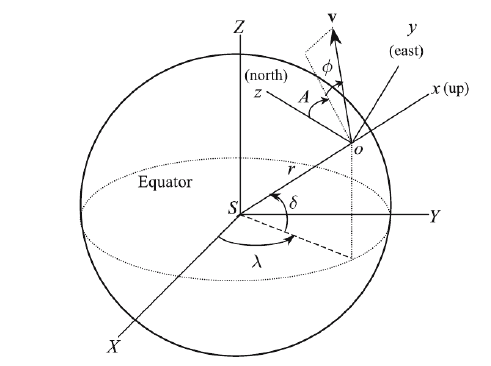
\includegraphics[scale=0.7]{imagenes/marco_teorico/LVLH.PNG}\\
	\end{center}
	\caption{ Sistema de referencia basado en la horizontal local.}
	\label{fig:LVLH}
	\footnotesize{Nota. Fuente \cite{cornelisse1979rocket}}
\end{figure}

\paragraph{Marco de Referencia Orbital (ORF):} Es un marco no inercial donde el origen coincide con el CG del satélite. El eje $X_o$ apunta hacia el centro de la Tierra (nadir). El eje $Y_o$ apunta en la dirección de la velocidad tangencialmente a la órbita. El eje $Z_o$ completa el sistema usando la regla de la mano derecha como se muestra en la \textbf{Fig. \ref{fig:marco_orbital}}.

\begin{figure}[!ht]
	\begin{center}
		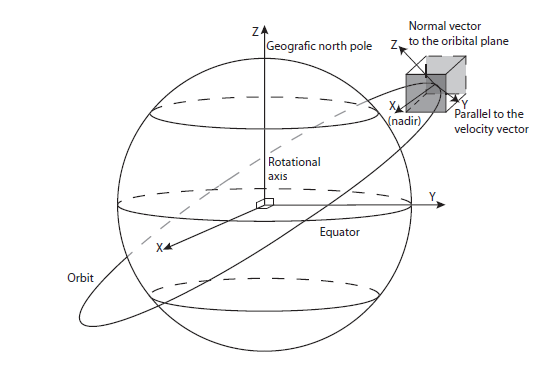
\includegraphics[scale=0.7]{imagenes/marco_teorico/marco_orbital.PNG}\\
	\end{center}
	\caption{ Marco Orbital.}
	\label{fig:marco_orbital}
	\footnotesize{Nota. Fuente \cite{Andresen2005}}
\end{figure}



\paragraph{Marco de Referencia centrado en el cuerpo (BRF):}Se fija con respecto al centro de masa del satélite \textbf({Fig. \ref{fig:marco_cuerpo}}). Se utiliza para determinar la orientación de los instrumentos a bordo. Si algunos de los instrumentos a bordo dependen de de la orientación del satélite, por ejemplo una cámara, es conveniente definir el BRF con uno de los ejes paralelos al campo de visión de este instrumento. Por otro lado, la orientación del satélite se describe en relación con el marco orbital como se ve en la \textbf{Fig. \ref{fig:marco_orbital_cuerpo}}.


\begin{figure}[!ht]
	\begin{center}
		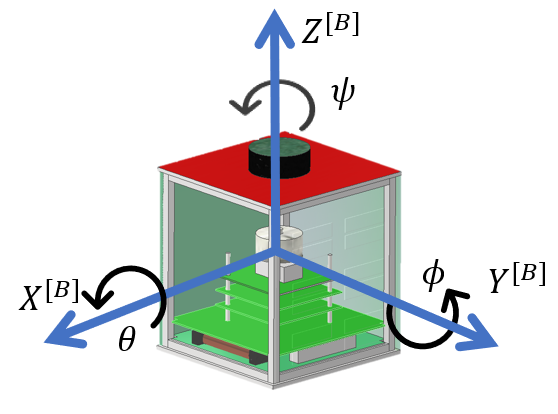
\includegraphics[scale=0.7]{imagenes/marco_teorico/marco_cuerpo.PNG}\\
	\end{center}
	\caption{ Marco de referencia centrado en el cuerpo. Adicionalmente se observan los ángulos roll ($\phi$), pitch ($\theta$) y yaw ($\psi$)}.
	\label{fig:marco_cuerpo}
%	\footnotesize{Nota. Fuente \cite{Andresen2005}}
\end{figure}

\begin{figure}[!ht]
	\begin{center}
		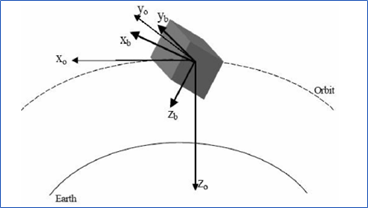
\includegraphics[scale=0.9]{imagenes/marco_teorico/orbital_cuerpo.PNG}\\
	\end{center}
	\caption{ Marco de referencia centrado en el cuerpo y marco orbital}
	\label{fig:marco_orbital_cuerpo}
		\footnotesize{Nota. Fuente \cite{Karatas2006}}
\end{figure}

\paragraph{Marco de Referencia centrado en la tierra (ECI):}Este marco está fijo en el espacio, por lo que es un marco de referencia no acelerado que permite la aplicación de las Leyes de Newton, donde su origen está situado en el centro de la Tierra. El eje Z apunta hacia el Polo Norte, el eje X hacia el Equinoccio de Primavera y el eje Y completa el sistema de coordenadas cartesianas como se ve en la \textbf{Fig. \ref{fig:ECI}}.
 
 \begin{figure}[!ht]
 	\begin{center}
 		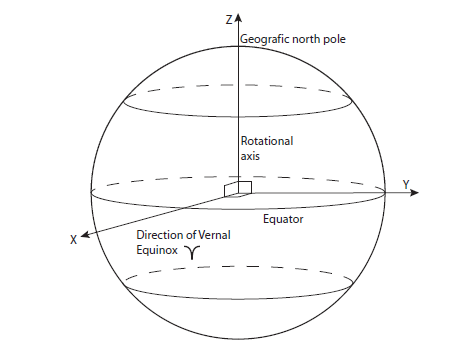
\includegraphics[scale=0.7]{imagenes/marco_teorico/ECI.PNG}\\
 	\end{center}
 	\caption{ Marco de referencia inercial centrado en la tierra (ECI)}
 	\label{fig:ECI}
 	\footnotesize{Nota. Fuente \cite{Andresen2005}}
 \end{figure}
 
Cuando se requiere considerar la rotación de la tierra, se recurre a un marco centrado y unido a la tierra (ECEF). Éste también se encuentra en el centro de la Tierra, sin embargo, los ejes X e Y giran con la tierra respecto al marco ECI alrededor del eje Z. El eje X apunta hacia la intersección del meridiano de Greenwich y el Ecuador. Finalmente, el eje Y completa el sistema siguiendo la regla de la mano derecha como se ve en la \textbf{Fig.\ref{fig:ECEF}}.


 \begin{figure}[!ht]
	\begin{center}
		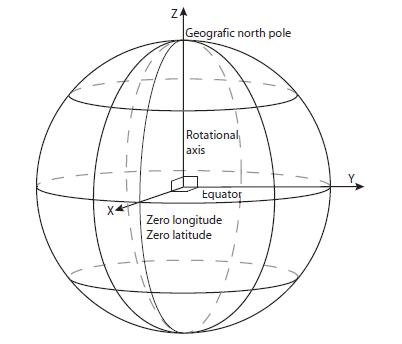
\includegraphics[scale=0.7]{imagenes/marco_teorico/ECEF.PNG}\\
	\end{center}
	\caption{ Marco de referencia fijo centrado en la tierra (ECEF)}
	\label{fig:ECEF}
	\footnotesize{Nota. Fuente \cite{Andresen2005}}
\end{figure}

Estos marcos de coordenadas permiten describir la actitud en términos de la orientación del BRF con respecto al ORF o ECI. Para ello se utiliza la representación de cuaterniones o ángulos de Euler en una matriz de cosenos directores (DCM) o matriz de transformación. Esta matriz permite transformar vectores de un sistema de referencia a otro como se verá en la siguiente sección.

\subsubsection{Transformación de marcos de referencia}
\hfill \break
Según la notación y formulación presentada en \cite{grewal2007global},  $C_{to}^{from}$ denota una matriz de transformación de coordenadas desde un
marco de coordenadas (designado por "from") a otro marco de coordenadas (designado por "to"). Por ejemplo $C_{BRF}^{ORF}$ denota la matriz de transformación de coordenadas desde el marco orbital al marco centrado en el cuerpo. Las matrices de transformación de coordenadas cumplen algunas propiedades útiles como:

\begin{itemize}
	
	\item La regla de composición que expresa que 
	\begin{equation}
		C_{C}^{B} C_{B}^{A} = C_{C}^{A}\label{eq:transformada1}
	\end{equation}
	donde A, B y C representan diferentes marcos de coordenadas.
	
	\item La inversa de una matriz de transformación es igual a su transpuesta, lo cual revierte la rotación del marco de referencia. Esto se expresa de la siguiente manera:
		\begin{equation}
			 \left(C_{C}^{B}\right)^T = \left(C_{C}^{B}\right)^{-1} = C_{B}^{C}\label{eq:transformada2}
		\end{equation}
		
\end{itemize}

En este sentido, se puede definir una expresión general para la transformación de coordenadas en 3 ejes. Para expresar el vector $\vec{v}$ en el marco $XYZ$ y se quiere expresar en el marco $UVW$ se tiene que:

$$
\left[\begin{array}{c}
	v_x\\
	v_y\\
	v_z
\end{array}\right] = 
C_{XYZ}^{UVW}
\left[\begin{array}{c}
	v_u\\
	v_v\\
	v_w
\end{array}\right]
$$

Donde
$$
C_{XYZ}^{UVW} = \left[\begin{array}{ccc}
	1_x^{T}1_u & 1_x^{T}1_v & 1_x^{T}1_w\\
	1_y^{T}1_u & 1_y^{T}1_v & 1_y^{T}1_w\\
	1_z^{T}1_u & 1_z^{T}1_v & 1_z^{T}1_w
\end{array}\right]
$$

De la expresión anterior, $1_{a}^{T}1_b$ representa el producto punto de un vector unitario del marco $XYZ$ con un vector unitario del marco $UVW$. Sin embargo, este producto punto también representa el ángulo entre ambos vectores, por lo que se tiene que $1_a^{T}1_b = cos\left(\theta_{ab}\right)$. Por este motivo, las matrices de transformación también son llamadas matrices de cosenos directores (DCM) y se define con la siguiente expresión:

$$
C_{XYZ}^{UVW} = \left[\begin{array}{ccc}
	cos\left(\theta_{xu}\right) &cos\left(\theta_{xv}\right) & cos\left(\theta_{xw}\right)\\
	cos\left(\theta_{yu}\right) &cos\left(\theta_{yv}\right) & cos\left(\theta_{yw}\right)\\
	cos\left(\theta_{zu}\right) &cos\left(\theta_{zv}\right) & cos\left(\theta_{zw}\right)
\end{array}\right]
$$
	

\subsubsection{Ángulos de Euler}
\hfill \break
La actitud de un vehículo puede representarse mediante los ángulos de roll ($\phi$), pitch ($\theta$) y yaw ($\psi$). Estos ángulos representan las rotaciones consecutivas sobre los ejes $X$, $Y$ y $Z$ con el fin de pasar de un marco a otro \textbf{(Fig.\ref{fig:angulosEuler})}. El orden en que estas rotaciones son efectuadas tienen efectos en la matriz de rotación.



\begin{figure}[!ht]
	\begin{center}
		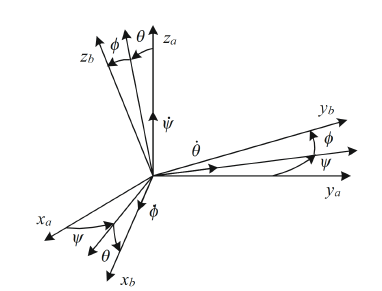
\includegraphics[scale=0.8]{imagenes/marco_teorico/angulos_euler.PNG}\\
	\end{center}
	\caption{ Ángulos de Euler : Roll-Pitch-Yaw }
	\label{fig:angulosEuler}
	\footnotesize{Nota. Fuente \cite{tes:Sorolla2019}}
\end{figure}

 Debido a que el problema discutido en este trabajo se restringió para solo un grado de libertad, solo basta realizar una rotacion de un ángulo $\phi$ en el eje $Z_o$ del marco orbital (ORF) para pasar al marco del cuerpo (BRF) como se vió en la  \textbf{Fig. \ref{fig:marco_cuerpo}}. Lo anterior puede lograrse con la matriz de transformación $R_{B}^{O}$:
$$
\mathbf{R_{B}^{O}}=\mathbf{R_{z,\psi}}=\left[\begin{array}{ccc}
	cos\psi & -sin\psi & 0 \\
	sin\psi & cos\psi & 0 \\
	0 & 0 & 1
\end{array}\right]
$$


%$$
%\mathbf{I}=\left[\begin{array}{ccc}
%	I_{x x} & I_{x y} & I_{x z} \\
%	I_{y x} & I_{y y} & I_{y z} \\
%	I_{z x} & I_{z y} & I_{z z}
%\end{array}\right]:\text { Matriz de inercia del CubeSat }
%$$
\subsubsection{Cuaterniones}
\hfill \break
Los ángulos de Euler pueden provocar singularidades en determinados ángulos cuando se utilizan en cálculos numéricos. A ese problema se le conoce intuitivamente como gimbal lock o bloqueo de Cardan. Como puede verse en el gimbal de la \textbf{Fig.\ref{fig:gimbal}}, puede darse el caso que dos ejes giren de forma paralela, perdiendo así un grado de libertad.

\begin{figure}[!ht]
	\begin{center}
		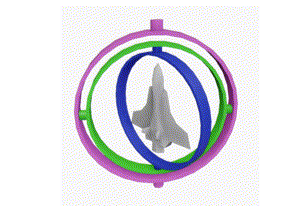
\includegraphics[scale=0.8]{imagenes/marco_teorico/gimbal.PNG}\\
	\end{center}
	\caption{ Gimbal compuesto por 3 cardanes, en esta configuración se presenta el bloqueo de 1 grado de libertad. }
	\label{fig:gimbal}
%	\footnotesize{Nota. Fuente \cite{tes:Sorolla2019}}
\end{figure}

Por este motivo, es mas conveniente usar los cuaterniones, ya que son una mejor representación sin singularidades y sin funciones trigonométricas en la matriz de transformación \cite{wertz1978spacecraft}. En este sentido, el conjunto de cuaterniones consta de cuatro parámetros, que se definen en términos del eje de Euler. El teorema de rotación del eje propio de Euler establece que la rotación finita de un cuerpo rígido con un punto fijo puede expresarse mediante una única rotación alrededor de algún eje fijo.

Este eje fijo, el eje de Euler, se representa mediante un vector unitario de componentes imaginarias $\hat{e} =(e_x,e_y,e_z)$ y una componente real $\eta$ donde $\Phi$ es el  ángulo de rotación sobre el eje de Euler. Esta representación se define como se evidencia desde la eq. (\ref{eq:cuaterniones}).

\begin{equation}
	\eta = cos\left(\frac{\Phi}{2}\right),
	\qquad
	\eta =\left[\begin{array}{c}
		\epsilon_1\\
		\epsilon_2\\
		 \epsilon_3
	\end{array}\right] =
	\left[\begin{array}{c}
		e_x sin\left(\Phi/2\right)\\
		e_y sin\left(\Phi/2\right)\\
		e_z sin\left(\Phi/2\right)
	\end{array}\right] ,
	\qquad
		q = \left[\begin{array}{c}
			\eta\\
		\epsilon_1\\
		\epsilon_2\\
		\epsilon_3
	\end{array}\right] 
	\label{eq:cuaterniones}
\end{equation}

%\begin{gather}
%%	$q1 = e_x sin(\Phi /2)$\label{eq:q1}\\[10pt]
%	q_1 = e_x sin\left(\dfrac{\Phi}{2}\right)\label{eq:q1}\\[10pt]
%	q_2 = e_y sin\left(\dfrac{\Phi}{2}\right)\label{eq:q2}\\[10pt]
%	q_3 = e_z sin\left(\dfrac{\Phi}{2}\right)\label{eq:q3}\\[10pt]
%	q_4 = cos\left(\dfrac{\Phi}{2}\right)\label{eq:q4}\\[10pt]
%\end{gather}

Donde se cumple que $\eta^2 + \epsilon_1^2+ \epsilon_2^2+ \epsilon_3^2 =1 $. Por otro lado, si se quiere pasar de ángulos de Euler a cuaterniones puede hacerse siguiendo la expresión (\ref{eq:euler2quat}).

\begin{equation}
q=\left[\begin{array}{c}
	\eta \\
	\epsilon_1 \\
	\epsilon_2 \\
	\epsilon_3
\end{array}\right]=\left[\begin{array}{l}
	c(\phi / 2) c(\theta / 2) c(\psi / 2)+s(\phi / 2) s(\theta / 2) s(\psi / 2) \\
	s(\phi / 2) c(\theta / 2) c(\psi / 2)-s(\phi / 2) c(\theta / 2) s(\psi / 2) \\
	c(\phi / 2) s(\theta / 2) c(\psi / 2)+s(\phi / 2) c(\theta / 2) s(\psi / 2) \\
	c(\phi / 2) c(\theta / 2) s(\psi / 2)-s(\phi / 2) s(\theta / 2) c(\psi / 2)
\end{array}\right]\label{eq:euler2quat}
\end{equation}


La transformacion de cuaterniones a angulos de Euler puede ser calculada con la expresión (\ref{eq:quat2euler}).

\begin{equation}
	\begin{gathered}
		\phi=\operatorname{atan}\left(2\left(q_2 q_3+\eta q_1\right),\left(\eta^2-q_1^2-q_2^2-q_3^2\right)\right) \\
		\theta=\operatorname{asin}\left(\left(q_1 q_3-\eta q_2\right)\right) \\
		\psi=\operatorname{atan}\left(2\left(q_1 q_2+\eta q_3\right),\left(\eta^2+q_1^2-q_2^2-q_3^2\right)\right)
	\end{gathered}\label{eq:quat2euler}
\end{equation}

Sin embargo, a diferencia de los ángulos de Euler, los cuaterniones no resultan tan intuitivos de interpretar, por lo tanto, serán usados en algunos cálculos numéricos que involucran la dinámica del CubeSat, pero tambien se recurriá a los ángulos de Euler para representar las rotaciones deseadas para el sistema de control.



\subsection{Teoría de Control}
Como se mencionó en la sección del ADCS, para garantizar la estabilidad de un satélite primero es necesario conocer su orientación angular en el BRF y determinar su actitud respecto al ORF. No obstante, la acción de los actuadores depende de la posición instantánea y sus cambios para poder compensar y anticipar el efecto de las perturbaciones en la actitud. Por tal motivo, los ADCS se fundamentan en la teoría de control.
De tal manera, la ingeniería de control recurre a los sistemas retroalimentados o en lazo cerrado, en los cuales, se alimenta al controlador con la señal de error de actuación, que es la diferencia entre la señal de entrada y la señal de realimentación (que puede ser la propia señal de salida o una función de la señal de salida y sus derivadas y/o integrales), con el fin de reducir el error y llevar la salida del sistema a un valor deseado \cite{ogata2010modern}. 
Así mismo, los sistemas en lazo cerrado tienen la habilidad de rechazar perturbaciones externas y mejorar la atenuación del ruido de medición. Las perturbaciones y el ruido de medición se incorporan en el diagrama de bloques como entradas externas, como se ilustra en la \textbf{Fig.\ref{fig:feedback}}.



\begin{figure}[!ht]
	\begin{center}
		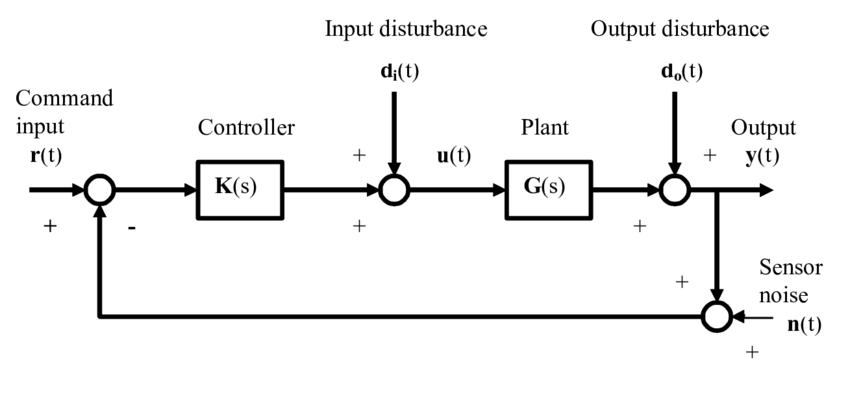
\includegraphics[scale=0.8]{imagenes/marco_teorico/lazo cerrado.PNG}\\
	\end{center}
	\caption{  Sistema en lazo cerrado con perturbaciones externas }
	\label{fig:feedback}
%	\footnotesize{Nota. Fuente \cite{tes:Sorolla2019}}
\end{figure}
\subsubsection{Modelo dinámico}

Para comprender y controlar sistemas complejos, es preciso obtener modelos matemáticos cuantitativos de dichos sistemas. Es necesario, pues, analizar las relaciones entre las variables del sistema y obtener un modelo matemático. Dado que los sistemas considerados son dinámicos, las ecuaciones descriptivas suelen ser ecuaciones diferenciales. Además, si estas ecuaciones se pueden linealizar, es posible utilizar la transformada de Laplace para simplificar el método de solución. En la práctica, debido a la complejidad de los sistemas y nuestro desconocimiento de todos los factores relevantes, se hace necesaria la introducción de suposiciones relativas al funcionamiento del sistema. Por lo tanto, a menudo resultará útil considerar el sistema físico, expresar y linealizar el sistema.
 
\subsection{Ambiente espacial en LEO}

La órbita baja (LEO, por sus siglas en inglés) es una región del espacio que se encuentra a una altitud de aproximadamente 160 a 2000 kilómetros sobre la superficie de la Tierra, como se muestra en la \textbf{Fig.\ref{fig:leo}}. Los satélites en LEO experimentan diversas condiciones ambientales, incluyendo gradientes de gravedad, arrastre aerodinámico, presión solar y el campo magnético terrestre. 


\begin{figure}[!ht]
	\begin{center}
		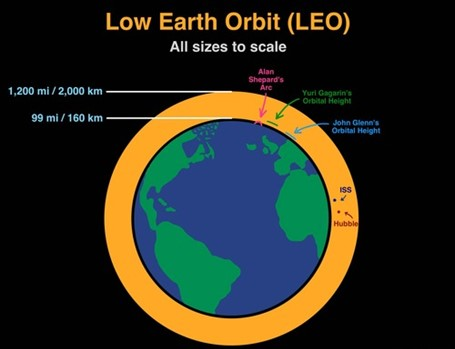
\includegraphics[scale=1]{imagenes/marco_teorico/leo.jpg}\\
	\end{center}
	\caption{  Órbita baja (LEO)}
	\label{fig:leo}
		\footnotesize{Nota. Fuente \cite{opc:LEO}}
\end{figure}

Los gradientes de gravedad son causados por la variación de la fuerza de gravedad a medida que el satélite se mueve a través de diferentes regiones del campo gravitacional. Esta variación decrece con el radio de la órbita a razón de $1/r^2$ por la ley de Newton. En este sentido, la parte baja de un satélite experimenta una atracción mayor que su parte superior, causando momentos de torsión no deseados y que tienden a alinear el eje del vehículo de menor inercia con el plano local vertical (LVLH) \cite{griffin2004space}, lo que puede afectar su orientación y estabilidad.

Por otro lado, el arrastre aerodinámico es causado por la interacción del satélite con la alta atmósfera, este arrastre genera un torque debido al desfase entre el centro de masa y el centro de presión del CubeSat. Por su parte, el campo geomagnético puede afectar la orientación y el control de los vehículos debido a los torques magnéticos. Estos últimos aparecen gracias a los lazos de corriente que generan dipolos y magnetizaciones residuales sobre el satélite\cite{Giesselman2006}. Adicionalmente, pueden presentarse otro tipo de perturbaciones debido a la radiación solar, ya que los fotones son desprendidos cuando se presenta actividad y erupciones en el sol.

Estos factores pueden afectar el sistema de control en LEO de diversas maneras. Por ejemplo, los gradientes de gravedad y el arrastre aerodinámico pueden causar momentos de torsión no deseados, lo que puede añade energía al sistema en forma de momento angular, afectando la precisión del sistema de control.
 
Para mitigar estos efectos, se utilizan diversas técnicas de control, como el control de actitud, que utiliza dispositivos como los ya mencionados magnetorquers, ruedas de reacción y propulsores para controlar la orientación. También se pueden utilizar técnicas de control adaptativo y control predictivo para compensar los efectos del arrastre aerodinámico y los gradientes de gravedad \cite{Junkins1997}.
Dado que el desempeño del ADCS se ve influenciado por las condiciones del ambiente espacial, es necesario conocer las particularidades de la órbita donde se encontrará el CubeSat. De esta manera, es posible incluir estos parámetros en el modelo dinámico y en los controladores que se evaluarán. 


%En esta sección se citan los autores que han tenido influencia directa en tu investigación. Recuerda, debes escoger solo un método para realizar las citas y referencias, es decir, debes seleccionar entre gestores especializados como Mendeley, Zotero, EndNote, etc., Microsoft Word, o “Manuales”; no se deben mezclar entre sí. Nuestra recomendación principal es Mendeley. Evita referenciar sitios como blogs, Wikipedia, Rincón del Vago, Monografías.com y demás portales web que no se consideran fuentes primarias. No limites tu búsqueda a una sola herramienta (por ejemplo, solo www.google.com). Realiza búsquedas en diferentes plataformas académicas, tales como:
%
%\begin{itemize}
%    \item \textbf{Catálogo Sistema de Bibliotecas UdeA:} material impreso que reposa en Bibliotecas UdeA, tales como libros, revistas, tesis, diccionarios, informes, etc.
%    \item\textbf{Bases de datos suscritas de la Biblioteca:} plataformas digitales con millones de documentos en texto completo.
%    \item\textbf{Bases de datos de libre acceso:} Google Scholar, Microsoft Academic, Google Books, Redalyc, Scielo, Dialnet, DOAJ, PubMed, Base Search, entre muchas más.
%    \item\textbf{Documentos con acceso restringido:} si requieres el texto completo de artículos o libros con acceso restringido, que por lo general se encuentran en bases de datos no suscritas por la Universidad de Antioquia, solicítalos en tu Biblioteca enviando título exacto, el DOI o la url del documento. Tenemos convenios nacionales e internacionales que nos permiten acceder a esta información.
%\end{itemize}
%
%Ejemplo de cita parafraseada, es decir, frase no textual adaptada con las palabras de quien escribe; esta forma de citación es la más adecuada en textos académicos, demuestran lectura, análisis y redacción propia \cite{sec:pediatria}. Ejemplo de “Cita textual menor a 40 palabras, al interior del párrafo; no utilice recurrentemente esta forma de citación, pues demuestra poco análisis y redacción propios” \cite[p. 9]{opc:ramirez}. Otros ejemplos aceptados en estilo IEEE 2020:
%
%En citas paráfrasis, es posible mencionar o no el o los autores en la oración, ejemplos: resultados demostrados por Arango \cite{sec:pediatria}, resultados demostrados mediante publicación científica \cite{sec:pediatria}. Cita en paráfrasis de dos autores, con o sin autor mencionado: datos suministrados por Ramírez y Guzmán \cite{opc:ramirez}, datos suministrados en revista académica \cite{opc:ramirez}. Cita en paráfrasis con tres o más autores con et al.: resultados publicados por Baker et al. \cite{art:baker}, resultados publicados en revista científica \cite{art:baker}. Cita con dos fuentes, cada una en corchetes y en orden numérico: ambos autores coinciden en estos datos \cite{opc:bbva}, \cite{opc:film}. Cita con tres fuentes o más, con corchetes para el primero y el último, en orden numérico y separados por guion: diversos autores coinciden en estos datos \cite{opc:bbva}–\cite{lib:ieee}. 
%
%Cita “textual menor a 40 palabras” \cite[p. 466]{art:espectador}, cita “textual menor a 40 palabras con páginas continuas o discontinuas” \cite[pp. 15-16]{tes:tesis}.  %[8, pp. 15-16). debe terminar en parentesis
%
%Cita de cita en paráfrasis mencionando o no autores: Quintero y González, citados por Rioja \cite{con:conferencia}, Quintero y González, citados por \cite{con:conferencia}. Cita textual mayor a 40 palabras sin comillas:
%
%
%    \begin{quotation}
%    Es importante destacar que la revisión realizada permitió definir el constructo a evaluar, es decir, especificar el concepto de la e-inclusión que se asume en la investigación, así como los factores que deben ser considerados para su evaluación. Lo anterior constituye el fundamento conceptual de la tesis y es la base para desarrollarla \cite[p. 107]{art:acimed}. 
%    \end{quotation}
%
%Cita textual o directa con más de 40 palabras (se omiten las comillas), bloque aparte, sangría 1.25 cms. Ya que IEEE no señala nada en particular de este caso, se adaptan de las normas APA. Datos estadísticos analizados con SPSS \cite{opc:ibm}. Procure no incurrir en la citación excesiva: 

\newpage
%--------------------------
%\subsection*{MÉTODO PARA ELABORAR CITAS Y REFERENCIAS}
%
%Recuerda, debes escoger solo un método para realizar las citas y las referencias, es decir, debes seleccionar entre un gestor especializado como Mendeley, Zotero o EndNote (confiabilidad alta), el gestor nativo Microsoft Word (confiabilidad media) o “manuales” (confiabilidad baja); no se deben mezclar entre sí, nuestra recomendación principal es Mendeley, pues te permite almacenar, subrayar e insertar notas en PDF´s, guardar fichas bibliográficas, elaborar citas y bibliografías en APA, Vancouver, IEEE y más de 1.000 estilos diferentes, exportar registros, compartir documentos, etc. Para mayor información de Mendeley.com y \LaTeX visitar:
%
%\url{http://tiny.cc/zzrnuz}
%
%La presente plantilla incluye los archivos requeridos para la construcción apropiada de las referencias bibliograficas bajo los parametros de las normas IEEE, todo se limita a modificar los campos del archivo \textit{refe.bib} segun las necesidades de su escrito. Aqui algunos ejemplos de los diferentes tipos de documentos referanciables.
%
%
%Refencia a un libro \cite{lib:libro}, a un artículo \cite{art:baker}, a una seccion de libro sin título \cite{sec:pediatria}, a un acta \cite{act:acta}, a una conferencia \citep{con:conferencia}, a un capítulo o páginas específicas con título propio de un libro\citep[pp. 7-10]{ent:entre_libro},  a un documento sin editorial \citep{fll:folleto}, a las memorias de una conferencia \citep{ina:articulo_en_acta}, a un informe técnico \citep{inf:informe_tecnico}, a un manual \citep{man:manual}, a una tesis doctoral \citep{phd:phd_tesis}, a una tesis de maestría \citep{tes:tesis}, a una web o información de internet \citep{web:web} y para otros tipos de referencias diferentes a las anteriores \cite{opc:film}. Para el listado de referencias, tenga en cuenta que el apellido principal será la última palabra en el campo \textit{author}; Si como autor no figura una persona sino una organización, al llenar el campo \textit{author} del archivo \textit{.bib}, use $\{\}$ dobles (ver referencia \citep{lib:ieee}).
%
%A continuación se muestra una de las referencias del archivo \textit{refe.bib}, donde \linebreak \textit{ent:entre\_libro} es el identificador de la misma y para referenciarla se debe escrbir el comando $\backslash cite\{ent:entre\_libro\}$ 
%
%\newpage
%\begin{verbatim}
%@inbook{ent:entre_libro,
%     author         = {Angela Zapata},
%     title          = {Titulo de libro},
%     chapter        = {},
%     pages          = {10-20},
%     publisher      = {Editor},
%     volume         = {},
%     series	        = {},
%     type           = {},
%     address        = {},
%     edition        = {},
%     year           = {20XX},
%     month          = {},
%     note           = {},
%     language       = {},
%     }
%\end{verbatim}
%
%Recuerde que \LaTeX , en la sección de referencias, solo muestra las que se han citado en su escrito; agregar la información en el archivo \textit{refe.bib} no implica que la referencia se muestre en su documento
%
%Por otro lado, para citar ecuaciones e información semejante dentro del texto use $\backslash ref\{\}$, por ejemplo (\ref{eq:maxwell}) o (\ref{eq:maxwell3})
%
%\begin{equation}\label{eq:maxwell}
%    \oint_C \vec{B}\cdot d \vec{l}=\mu_0\int_S \vec{J}\cdot d \vec{s}+\mu_0\epsilon_0\dfrac{d }{d t}\int_S \vec{E}\cdot d \vec{s}
%\end{equation}
%
%y a su vez
%
%\begin{gather}
%    \vec{\nabla}\cdot \vec{E}= \dfrac{\rho}{\epsilon_0}\\
%    \vec{\nabla}\cdot \vec{B}= 0\\
%    \vec{\nabla}\times\vec{E}=-\dfrac{\partial\vec{B}}{\partial t}\\
%    c^2\vec{\nabla}\times\vec{B} =\dfrac{\vec{J}}{\epsilon_0}+\dfrac{\partial
%\vec{E}}{\partial t}\label{eq:maxwell3}\\
%    \vec{\nabla}\times \vec{B}=\mu_0\vec{J}+\mu_0 \epsilon_0 \dfrac{\partial \vec{E}}{\partial t}
%\end{gather}


\newpage
%--------------------------
\section{METODOLOGÍA}

%En la metodología se establecen los enfoques de investigación, esto es, cuantitativo, cualitativo o mixto.
La estrategia metodológica tiene un enforque cuantitativo, ya que toma como punto de partida un fenómeno, que puede ser amplio en el campo de la dinámica de satélites, pero que se acota cada vez más según se definen las preguntas de investigación, su alcance y su definición de variables. Por otro lado, se define un conocimiento mínimo, consolidado en el marco teórico, y una revisión de los métodos e investigaciones que se han realizado hasta el momento, consignado en el estado del arte.
En este sentido, el desarrollo de este trabajo de grado se divide en tres etapas:
\subsection{Modelo dinámico} 
Primero es necesario interpretar el fenómeno de estudio, partiendo de la realidad y llevándola a un entorno matemático que permita su simulación. Para ello se recurre a un modelo dinámico, constituido por las ecuaciones diferenciales involucradas en el fenómeno físico y sus propiedades inerciales.
De esta manera se pretende resolver las siguientes preguntas: ¿Cuál es el marco de referencia idóneo para plantear las ecuaciones del modelo dinámico? ¿De qué manera se puede comprobar que el modelo dinámico se acerca al modelamiento real del fenómeno? ¿Qué torques internos y externos deben tenerse en cuenta según las necesidades del proyecto?
Para ello se plantean las siguientes actividades:
\begin{enumerate}[label=\alph*)]
	
	\item Recopilación y comprensión de modelos dinámicos similares al caso de estudio según el estado del arte. Para esto se consultarán diversas fuentes de libros, bases de datos y revistas indexadas.
	
	\item Adaptación de dichos modelos para la construcción de un modelo propio: se parte de un modelo simple y se hacen suposiciones como: orbita circular, campo magnético constante, simetrías, etc.
	
	\item Simulación realizando ajustes de parámetros usando la herramienta computacional de Matlab Simulink: se busca conocer el comportamiento del modelo dinámico que corresponda a la realidad.

	
\end{enumerate}



\subsection{Diseño de estrategia de control} 
Una vez se tiene un modelo dinámico, se realizarán simulaciones con diferentes estrategias de control que garanticen condiciones de estabilidad e incluyan la desaturación de ruedas de reacción. 
De tal manera que, en la medida que se realicen y se desarrollen las simulaciones esta etapa se responderán las preguntas: ¿Qué estrategia de control es la que más se emplea actualmente? ¿Qué deficiencias tiene?, comparando la estrategia de control de referencia ¿cómo se desempeñan los otros controladores? Para esto se proponen las siguientes actividades y experimentos:

\begin{enumerate}[label=\alph*)]
	
	\item	Búsqueda bibliográfica de controladores para justificar para identificar aquellos que comúnmente utilizados para hacer frente al fenómeno de estudio. De esta manera, se seleccionará el controlador más usado para usarlo como punto de comparación. 
	\item	Definir índices de desempeño del comportamiento de los controladores justificando la incorporación de las diferentes variables que hacen parte de este, teniendo en cuenta parámetros como el consumo energético, el tiempo de reacción y error en estado estable.
	\item	Diseño y simulación de controladores de actitud con desaturación de RW, como por ejemplo LQR, PID, anti wind up Multi agente, modelo predictivo, static input allocation.
	\item	Definir escenarios: Se plantearán diferentes escenarios correspondientes a un uso específico del cubesat, donde el objetivo varía según la órbita o el perfil de misión. De esta manera se evaluará el desempeño de los controladores para distintas aplicaciones, como un apuntamiento constante hacia una base terrena, disminución de consumo energético o aumento en la respuesta para alcanzar la estabilidad.
	\item	Realizar pruebas con los diferentes controladores en los diferentes escenarios propuestos y compararlos a partir de sus índices de desempeño.
	
	
\end{enumerate}
 
 \subsection{Análisis de órbitas} 

Como se mencionó en la sección de modelo dinámico, este parte de realizar suposiciones y simplificaciones. Algunas de estas conciernen la órbita y las perturbaciones del medio ambiente espacial. En esta etapa se quiere determinar la influencia de ciertos parámetros orbitales de la órbita baja, sus correspondientes intensidades de campo geomagnético y como éstas afectan el desempeño de los magnetorquers en el fenómeno de desaturación.  
Luego de implementar condiciones de ambiente espacial, las simulaciones deberían dilucidar las siguientes preguntas: ¿En qué órbitas de presenta un mejor desempeño por parte de los magnetorquers y con cual controlador? ¿Qué tipo de perfil de misiones son las más indicadas para los controladores seleccionados? Para ello se plantean las siguientes actividades y experimentos:
\begin{enumerate}[label=\alph*)]
	
	\item	Integrar las intensidades de campo magnético terrestre según una órbita deseada en el modelo dinámico, a partir de recursos como el paquete SEET del software multifísico STK o su alternativa de código abierto GMAT, entre otros de uso libre. 
	\item	Nuevamente realizar pruebas y comparaciones de los controladores de actitud con desaturación de RW basados en los índices de desempeño. De esta manera, se evalúan diferentes escenarios donde se varían espacial y temporalmente algunos parámetros orbitales como la inclinación, excentricidad y la variación del campo geomagnético.
	
	
\end{enumerate}

Finalmente, el esquema de la estrategia metodológica puede apreciarse en la Fig.\ref{fig:metodologia}, donde se plantea el entregable u objetivo a cumplir al término cada etapa, el cual es fundamental para el desarrollo de la etapa posterior. De esta manera se consolida una estrategia secuencial pero que puede estar sujeta a diferentes iteraciones según el desarrollo de las actividades.

\newpage
\begin{figure}[!ht]
	\begin{center}
		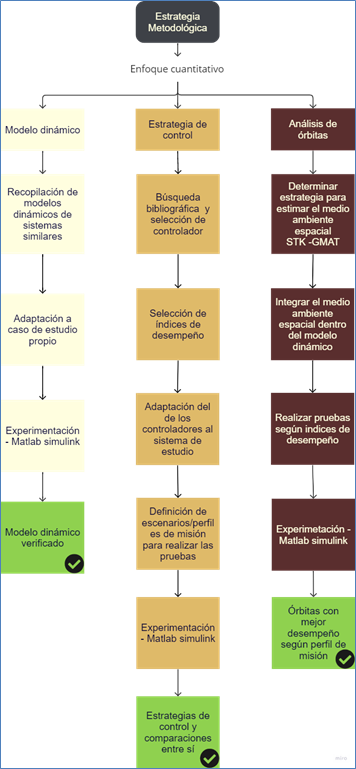
\includegraphics[scale=0.8]{imagenes/metodologia/grafico_metodologia.png}\\
	\end{center}
	\caption{Diagrama estrategia metodológica}
	\label{fig:metodologia}
	\textit{}
\end{figure}


\newpage
\section{MODELO DINÁMICO}
La de actitud de una nave espacial como un CubeSat puede ser representada por las ecuaciones dinámicas de Newton-Euler, las cuales describen los efectos de los torques externos e internos que modifican la aceleración del satélite. Para llegar a dichas ecuaciones se parte de la dinámica rotacional tal como se describen en \cite{Griffin2004}.

\begin{figure}[!h]
	\begin{center}
		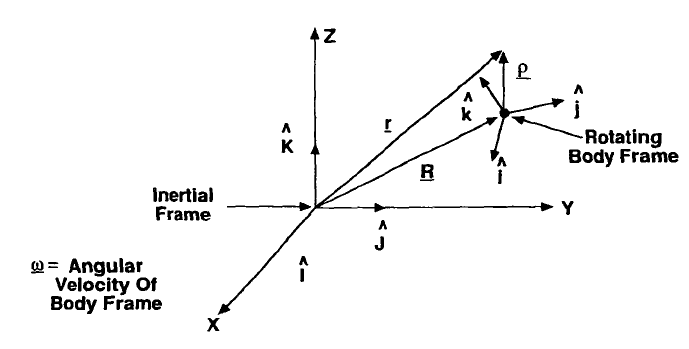
\includegraphics[scale=0.6]{imagenes/modelo_dinamico/ref_system.PNG}\\
	\end{center}
	\caption{Variación en el tiempo de un marco de referencia rotante}
	\label{fig:rot_frame}
	\textit{}
\end{figure}

La Fig.\ref{fig:rot_frame} muestra la geometría esencial del sistema. Se tiene el vector de posición $\rho$ en el marco del cuerpo en rotación, si se desea conocer su variación en el tiempo respecto al marco inercial se tiene:

\begin{equation}\label{eq:variacion_rho}
	\left(\frac{\mathrm{d} \rho}{\mathrm{d} t}\right)_i=\left(\frac{\mathrm{d} \rho}{\mathrm{d} t}\right)_b+\omega \times \boldsymbol{\rho}
\end{equation}

Donde $\omega$ es la velocidad angular en el marco del cuerpo. Por otro lado, se requieren determinar el vector posición $\vec{r}$ y sus derivadas $\vec{v}$ y $\vec{a}$. Del sistema vectorial se tiene una relación entre r y p:

\begin{equation}\label{eq:suma_vectores}
	r = R + \rho
\end{equation}

De esta manera, velocidad y la aceleración pueden ser determinadas: 

\begin{gather}
		\boldsymbol{v}=\left(\frac{\mathrm{d} \boldsymbol{r}}{\mathrm{d} t}\right)_i=\frac{\mathrm{d} \boldsymbol{R}}{\mathrm{d} t}+\left(\frac{\mathrm{d} \boldsymbol{\rho}}{\mathrm{d} t}\right)_b+\omega \times \boldsymbol{\rho}\label{eq:velocidad}\\[10pt]			
		\boldsymbol{a}=\left(\frac{\mathrm{d}^2 \boldsymbol{r}}{\mathrm{d} t^2}\right)_i=\frac{\mathrm{d}^2 \boldsymbol{R}}{\mathrm{d} t^2}+\left(\frac{\mathrm{d}^2 \boldsymbol{\rho}}{\mathrm{d} t^2}\right)_b+2 \omega \times\left(\frac{\mathrm{d} \boldsymbol{\rho}}{\mathrm{d} t}\right)_b+\frac{\mathrm{d} \omega}{\mathrm{d} t} \times \boldsymbol{\rho}+\omega \times(\omega \times \boldsymbol{\rho})\label{eq:aceleracion}				
\end{gather}

En la dinámica rotacional, dos cantidades fundamentales de interés son el momento de inercia y el momento angular. El momento angular de una colección de puntos de masa es el momento de su momento lineal alrededor de un origen definido. A partir de Fig.\ref{fig:rot_frame}, el momento angular de la masa mi alrededor del origen en el sistema de inercial es:

\begin{equation}
	H_{t}=\sum r_i \times m_i v_i\\
\end{equation}

Si aplicamos las eq.(\ref{eq:velocidad}) y eq.(\ref{eq:aceleracion}) con $V =\frac{\mathrm{d} {R}}{\mathrm{d} t}$ y si suponemos que 1) el origen del marco de rotación se encuentra en el centro de masa del cuerpo ($\sum m_i\rho_i =0$), y 2) los vectores de posición $\rho_i$ están fijos en el marco del cuerpo, es decir, tenemos un cuerpo rígido $\frac{\mathrm{d} {\rho}}{\mathrm{d} t} =0$ . Se obtiene el momento angular total así:

\begin{equation}\label{eq:H_total}
H_{t}=\left(\sum m_i\right)R\times V +\sum m_i \rho_i\times\frac{\mathrm{d} {\rho_i}}{\mathrm{d} t} = H_{orb} + H_b \\
\end{equation}

El primer término de la derecha es el momento angular del cuerpo rígido debido a su velocidad traslacional V en el marco de inercia. El segundo término es el momento angular del cuerpo debido a su velocidad de rotación alrededor de su propio centro de masa. La eq. (\ref{eq:H_total}) provee un importante resultado ya que indica que, en un cuerpo rígido, es posible escoger un marco de coordenadas que desacopla el momento angular del cuerpo y del momento angular orbital.
Por tal motivo, el análisis se centrará únicamente en el segundo término, donde la eq.(\ref{eq:variacion_rho}) se simplificaría de la siguiente manera: 

\begin{equation}\label{eq:variacion_rho_simplificada}
	\frac{\mathrm{d} \rho_j}{\mathrm{d} t}=\omega\times\rho_i
\end{equation}

De esta manera, a partir de la eq.(\ref{eq:H_total}) tenemos que el momento angular en el marco del cuerpo es:

\begin{equation}\label{eq:H_total_simplificada}
	H=\sum m_i\rho_i\times\frac{\mathrm{d} {\rho_i}}{\mathrm{d} t} =
	 \sum m_i\rho_i \times(\omega \times \rho_i) = I\omega \\
\end{equation}
Donde $I$ es una matriz real y simétrica, llamada matriz de inercia, con componentes: 
 
 $$
 \begin{aligned}
 	& I_{11}=\sum m_i\left(\rho_{i 2}^2+\rho_{i 3}^2\right) \\
 	& I_{22}=\sum m_i\left(\rho_{i 1}^2+\rho_{i 3}^2\right) \\
 	& I_{33}=\sum m_i\left(\rho_{i 1}^2+\rho_{i 2}^2\right) \\
 	& I_{12}=I_{21}=-\sum m_1 \rho_{i 1} \rho_{i 2} \\
 	& I_{13}=I_{31}=-\sum m_i \rho_{i 1} \rho_{i 3} \\
 	& I_{23}=I_{32}=-\sum m_i \rho_{i 2} \rho_{i 3}
 \end{aligned}
 $$
 
 La eq.(\ref{eq:H_total_simplificada}) nos indica que el momento angular total depende de la matriz de inercia del cubesat y del vector de velocidades angulares. Sin embargo, es necesario introducir el efecto de las ruedas de reacción, las cuales también disponen de un momento angular $h_w$. Por lo tanto, se tiene a partir de la eq.(\ref{eq:H_total_simplificada}) que: 
 
 \begin{equation}\label{eq:H_total_RW}
 	H = I\omega_b + h_w
 \end{equation}
 
 Por otro lado, el efecto de los torques externos se incluye al considerar una fuerza $F_i$ aplicada en una posición $\rho_i$ en las coordenadas del marco del cuerpo. Esta fuerza tiene un efecto dado por: 
  
 \begin{equation}
 	T_i=\rho_i \times F_i  
 \end{equation}
 
 
En este sentido, el torque neto de fuerzas externas es:

\begin{equation}
	T_{ext}=\sum \rho_i \times F_i=\sum \rho_i \times m_i \frac{\mathrm{d}^2 r_i}{\mathrm{~d} t^2} 	
\end{equation}
 
 
 Al expandir la expresión para la aceleración tal como se hizo en la eq.(\ref{eq:aceleracion}), se tiene que :
 
 \begin{equation}
 	T_{ext}= \frac{\mathrm{d} H}{\mathrm{d} t} = \left(\frac{\mathrm{d} H}{\mathrm{d} t}\right)_{body} + \omega \times H 	
 \end{equation}
 
 O visto de otra manera, asumiendo un marco fijo del cuerpo con ejes principales, se puede expresar el cambio del momento angular como el efecto de los torques y el producto cruz entre la velocidad angular y el momento angular total del sistema.
 
  \begin{equation}\label{eq:H_dot_1}
 	 \left(\frac{\mathrm{d} H}{\mathrm{d} t}\right)_{body} = T_{ext}-\omega \times \left(I\omega + h_w\right) 	
 \end{equation}
 
 Análogamente, se puede obtener otra expresión para el cambio de momento angular al derivar la \textbf{eq.(\ref{eq:H_total_RW})} respecto al tiempo :
 
 \begin{equation}\label{eq:H_dot_2}
 	\dot{H_b} = \left(\frac{\mathrm{d} H}{\mathrm{d} t}\right)_{body} = 
 	I\frac{\mathrm{d} \omega_b}{\mathrm{d} t} + \dot{h_w}  	
 \end{equation}
 
Tomando el principio del intercambio de momentos, se tiene que el momento angular producido por las ruedas de reacción se aplica al satélite con signo opuesto. Entonces si definimos $T_c$ como el par de control:

\begin{equation}\label{eq:torque_h}
	\dot{h_w} = T_c  	
\end{equation}

Al igualar las ecuaciones (\ref{eq:H_dot_1}) y (\ref{eq:H_dot_2}) se obtiene una expresión para las aceleraciones angulares, conocida como ecuación dinámica de Newton-Euler, la cual consolida el modelo dinámico del CubeSat:


\begin{equation}\label{eq:modelo_dinamico}
	\begin{aligned}
		& \frac{d \omega_b}{d t}=I^{-1}\left[-\omega_b \times\left(I \omega_b+h_w\right)+T_{ext}+T_c\right]\\[10pt]
		& \dot{\omega_b}=I^{-1}\left[-S(\omega)\left(I \omega_b+h_w\right)+T_{ext}+T_c\right]
	\end{aligned}
\end{equation}

donde:
$$
\mathbf{I}=\left[\begin{array}{ccc}
	I_{x x} & I_{x y} & I_{x z} \\
	I_{y x} & I_{y y} & I_{y z} \\
	I_{z x} & I_{z y} & I_{z z}
\end{array}\right]:\text { Matriz de inercia del CubeSat }
$$

$\mathbf{\omega_b}=\left[\begin{array}{l}\omega_x \\ \omega_y \\ \omega_z\end{array}\right]:$ Vector de velocidad angular del satélite en el marco del cuerpo.\\[5pt]	

$\mathbf{h_w}=\left[\begin{array}{l}h_x \\ h_y \\ h_z\end{array}\right]:$ Vector de momento de angular de las RW.\\[10pt]	

\noindent Realizando las respectivas multiplicaciones matriciales, se tienen las ecuaciones en cada eje:

\begin{gather}	
	\dot{\omega}_x=\left[T_x+T_{C x}+\omega_y \omega_z\left[I_{y y}-I_{z z}\right]-h_z \omega_y+h_y \omega_z\right] / I_{x x}\label{eq:modelo_dinamico_x}\\
	\dot{\omega}_y=\left[T_y+T_{C y}+\omega_x \omega_z\left[I_{z z}-I_{x x}\right]-h_x \omega_z+h_z \omega_x\right] / I_{y y}\label{eq:modelo_dinamico_y}\\
	\dot{\omega}_z=\left[T_z+T_{C z}+\omega_x \omega_y\left[I_{x x}-I_{y y}\right]-h_y \omega_x+h_x \omega_y\right] / I_{z z}
\end{gather}


Finalmente, usando las componentes del vector de velocidades angulares es posible determinar la actitud del CubeSat. La interpretación de los ángulos de Euler es más intuitiva, pero para evitar que surjan singularidades, los cuaterniones resultan mas convenientes para los cálculos de simulación \cite{Steyn2011}. La ecuación diferencial cinemática de los cuaterniones está descrita en la  \textbf{eq.(\ref{eq:modelo_cinematico})}: 

\begin{equation}\label{eq:modelo_cinematico}
	\dot{\mathbf{q}}=\frac{1}{2} \Omega \mathbf{q} \\
\end{equation}

Donde:
 

\begin{center}
	$\Omega$ = $\left[\begin{array}{cccc}
		0 & w_z & -w_y & w_x \\
		-w_z & 0 & w_x & w_y \\
		w_y & -w_x & 0 & w_z \\
		-w_x & -w_y & -w_z & 0
	\end{array}\right],
	\qquad
	\mathbf{q}=\left[\begin{array}{llll}
		q_1 & q_2 & q_3 & q_4
	\end{array}\right]^T
	$
\end{center}

En la \textbf{Fig. \ref{fig:din_sc}} se evidencia la implementación de la \textbf{eq.(\ref{eq:modelo_dinamico})} en Simulink, donde se tienen como salidas tanto las ecuaciones cinemáticas, que relacionan velocidades angulares $\omega$, como las ecuaciones dinámicas, las cuales determinan la actitud del satélite por medio de los cuaterniones $q$.


\begin{figure}[!h]
	\begin{center}
		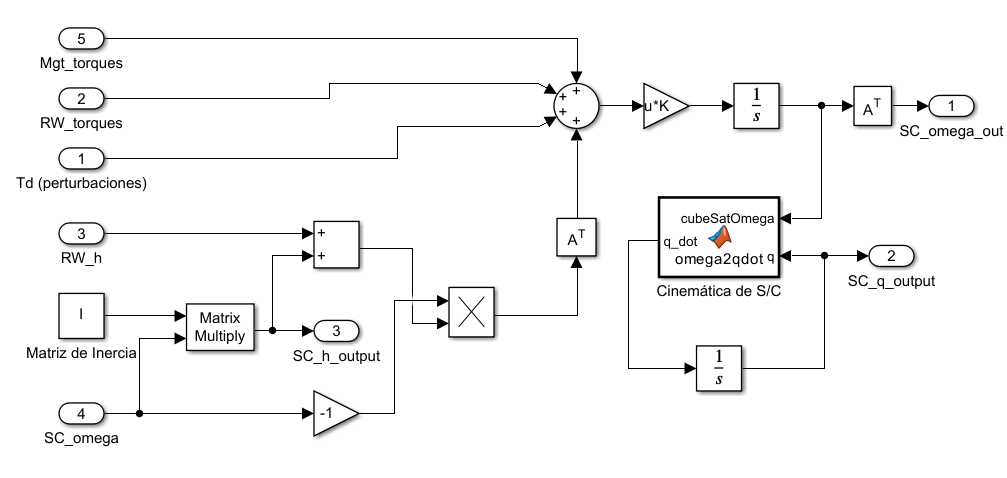
\includegraphics[scale=0.6]{imagenes/modelo_dinamico/dinamica_satelite.PNG}\\
	\end{center}
	\caption{Implementación modelo dinámico en Simulink.}
	\label{fig:din_sc}
	\textit{}
\end{figure}

En la siguiente sección se profundizará en como determinar parámetros fundamentales del modelo dinámico, sintetizado en la eq. (\ref{eq:modelo_dinamico}), como la matriz de inercia del EyasSat, el modelo de los actuadores del ADCS y el cálculo de perturbaciones. 

\newpage
\subsection{PROPIEDADES INERCIALES}

%Fotos y diseño CAD

Con el fin de obtener la matriz de inercia del EyasSat se realizó un CAD en el software Inventor\textsuperscript{\tiny\textregistered}. Para ello se desarmó el Cubesat con el fin de conocer las dimensiones de las tarjetas integradas donde se encuentran los diferentes subsistemas \textbf{(Fig. \ref{fig:eyassat_lab})}. De igual forma, como se evidencia en la \textbf{Fig. \ref{fig:mediciones}}, los pesos de cada tarjeta fueron registrados para realizar el cálculo de la matriz de inercia a partir de la distribución de masa de los componentes.


\begin{figure}[h]
	\centering
	\subfloat[Ensamble EyasSat.]{
		\label{f:cube_armado}
		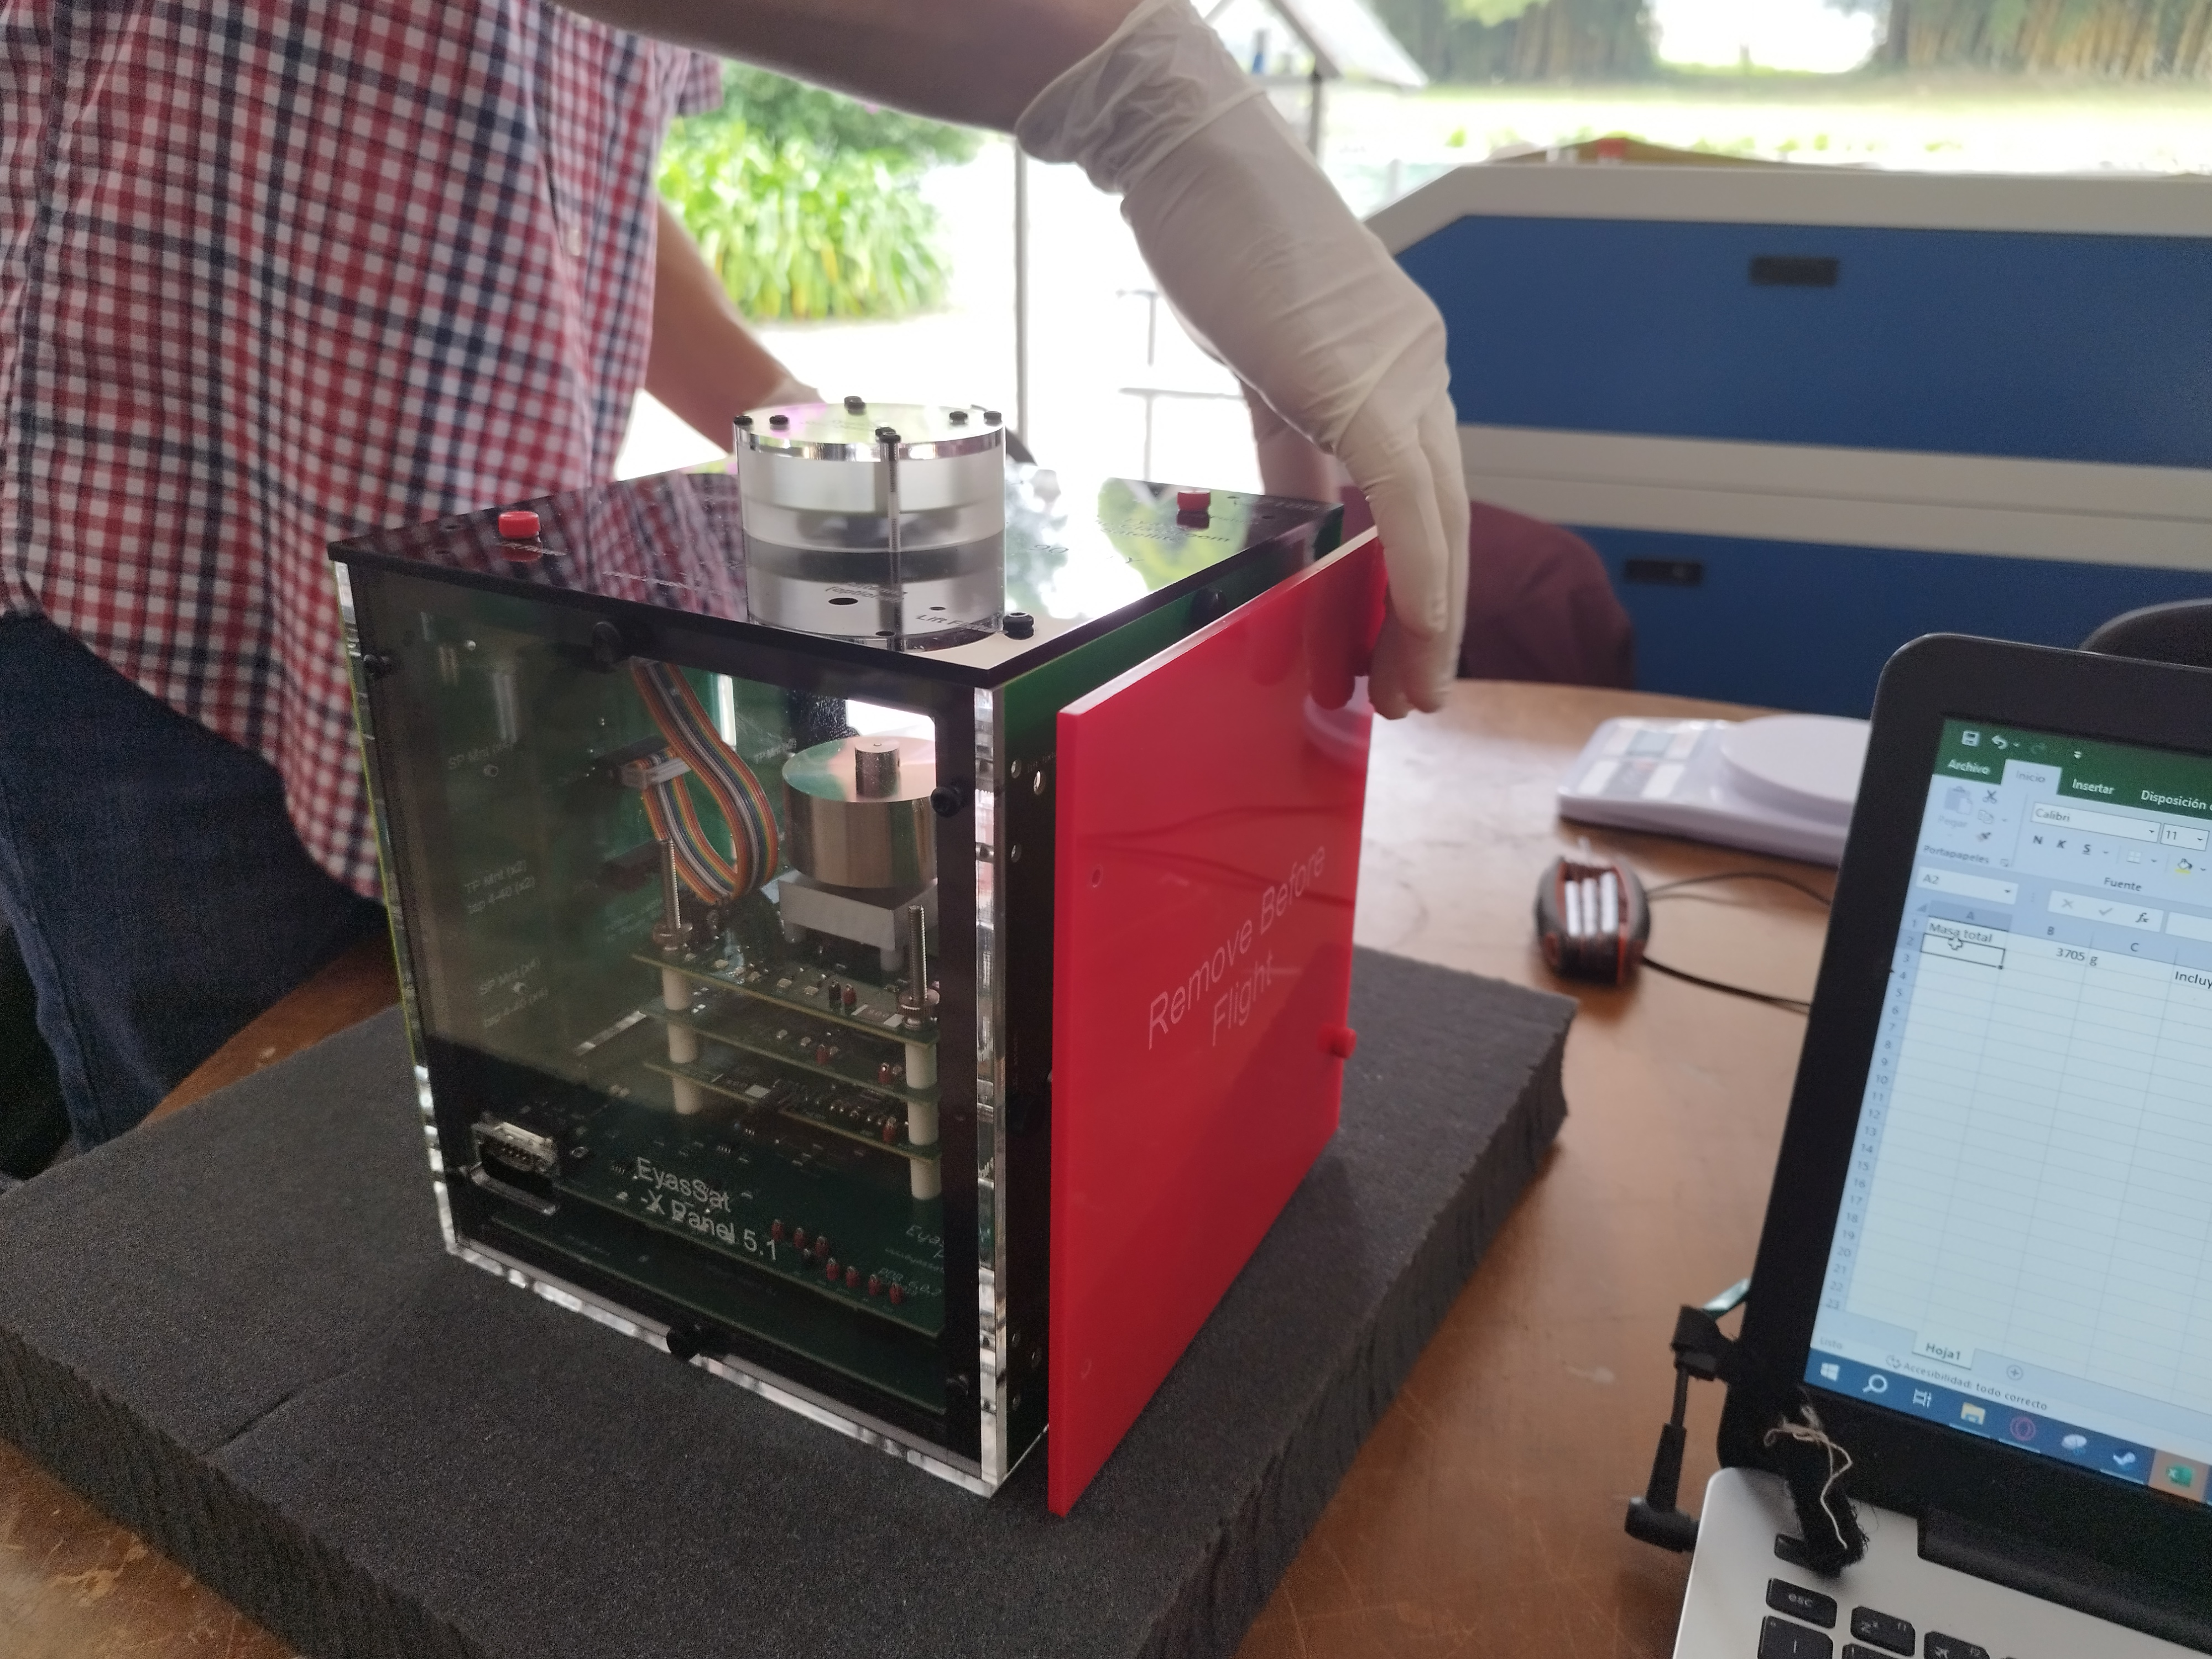
\includegraphics[width=0.45\textwidth]{imagenes/modelo_dinamico/eyassat_armado.jpg}}
	\subfloat[Tarjetas integradas que componen los módulos del EyasSat. ]{
		\label{f:cube_desarmado}
		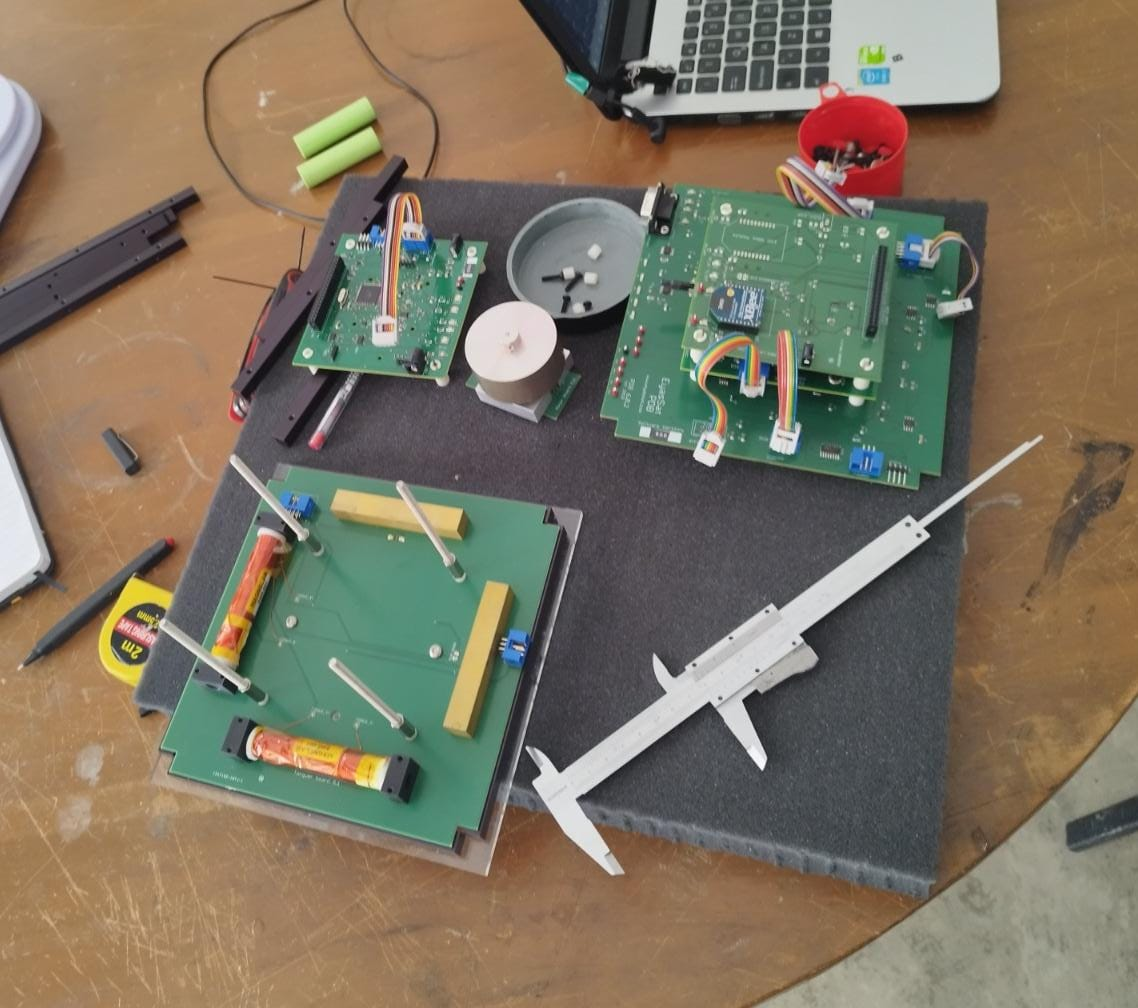
\includegraphics[width=0.382\textwidth]{imagenes/modelo_dinamico/capas.jpeg}}
	
	\caption{Cálculo de matriz de inercia.}
	\label{fig:eyassat_lab}
\end{figure}

Como resultado de este ejercicio, se determinó que el EyasSat tiene una masa total de $3.705$ $kg$ y los valores de la diagonal principal de la matriz de inercia se calcularon como se evidencia en la \textbf{Tabla \ref{table:inercia_eyassat}}.
\begin{table}[h]
	\caption{\MakeUppercase{Inercias EyasSat}}
	\begin{center}
		\begin{tabular}{ c c}
			
			Componente & Inercia [$kg\cdot m^2$] \\ \hline
			$I_{xx}$ &  $3.361\cdot10^{-2}$ \\ 
			$I_{yy}$ &  $3.082\cdot10^{-2}$ \\ 
			$I_{zz}$ &  $2.717\cdot10^{-2}$ \\ \hline
	
		\end{tabular}
	\end{center}
	\label{table:inercia_eyassat}
\end{table}

Debido a que la inercia se midió a partir del centro de masa, los productos de inercia pueden despreciarse. Finalmente, el CAD se incluyó en el entorno de 3D World Editor de Simulink\textsuperscript{\tiny\textregistered} como se aprecia en la \textbf{Fig. \ref{fig:escenario}}.


\begin{figure}[h!]
	\centering
	\subfloat[Ensamble del módulo ADCS.]{
		\label{fig:medicion_capas}
		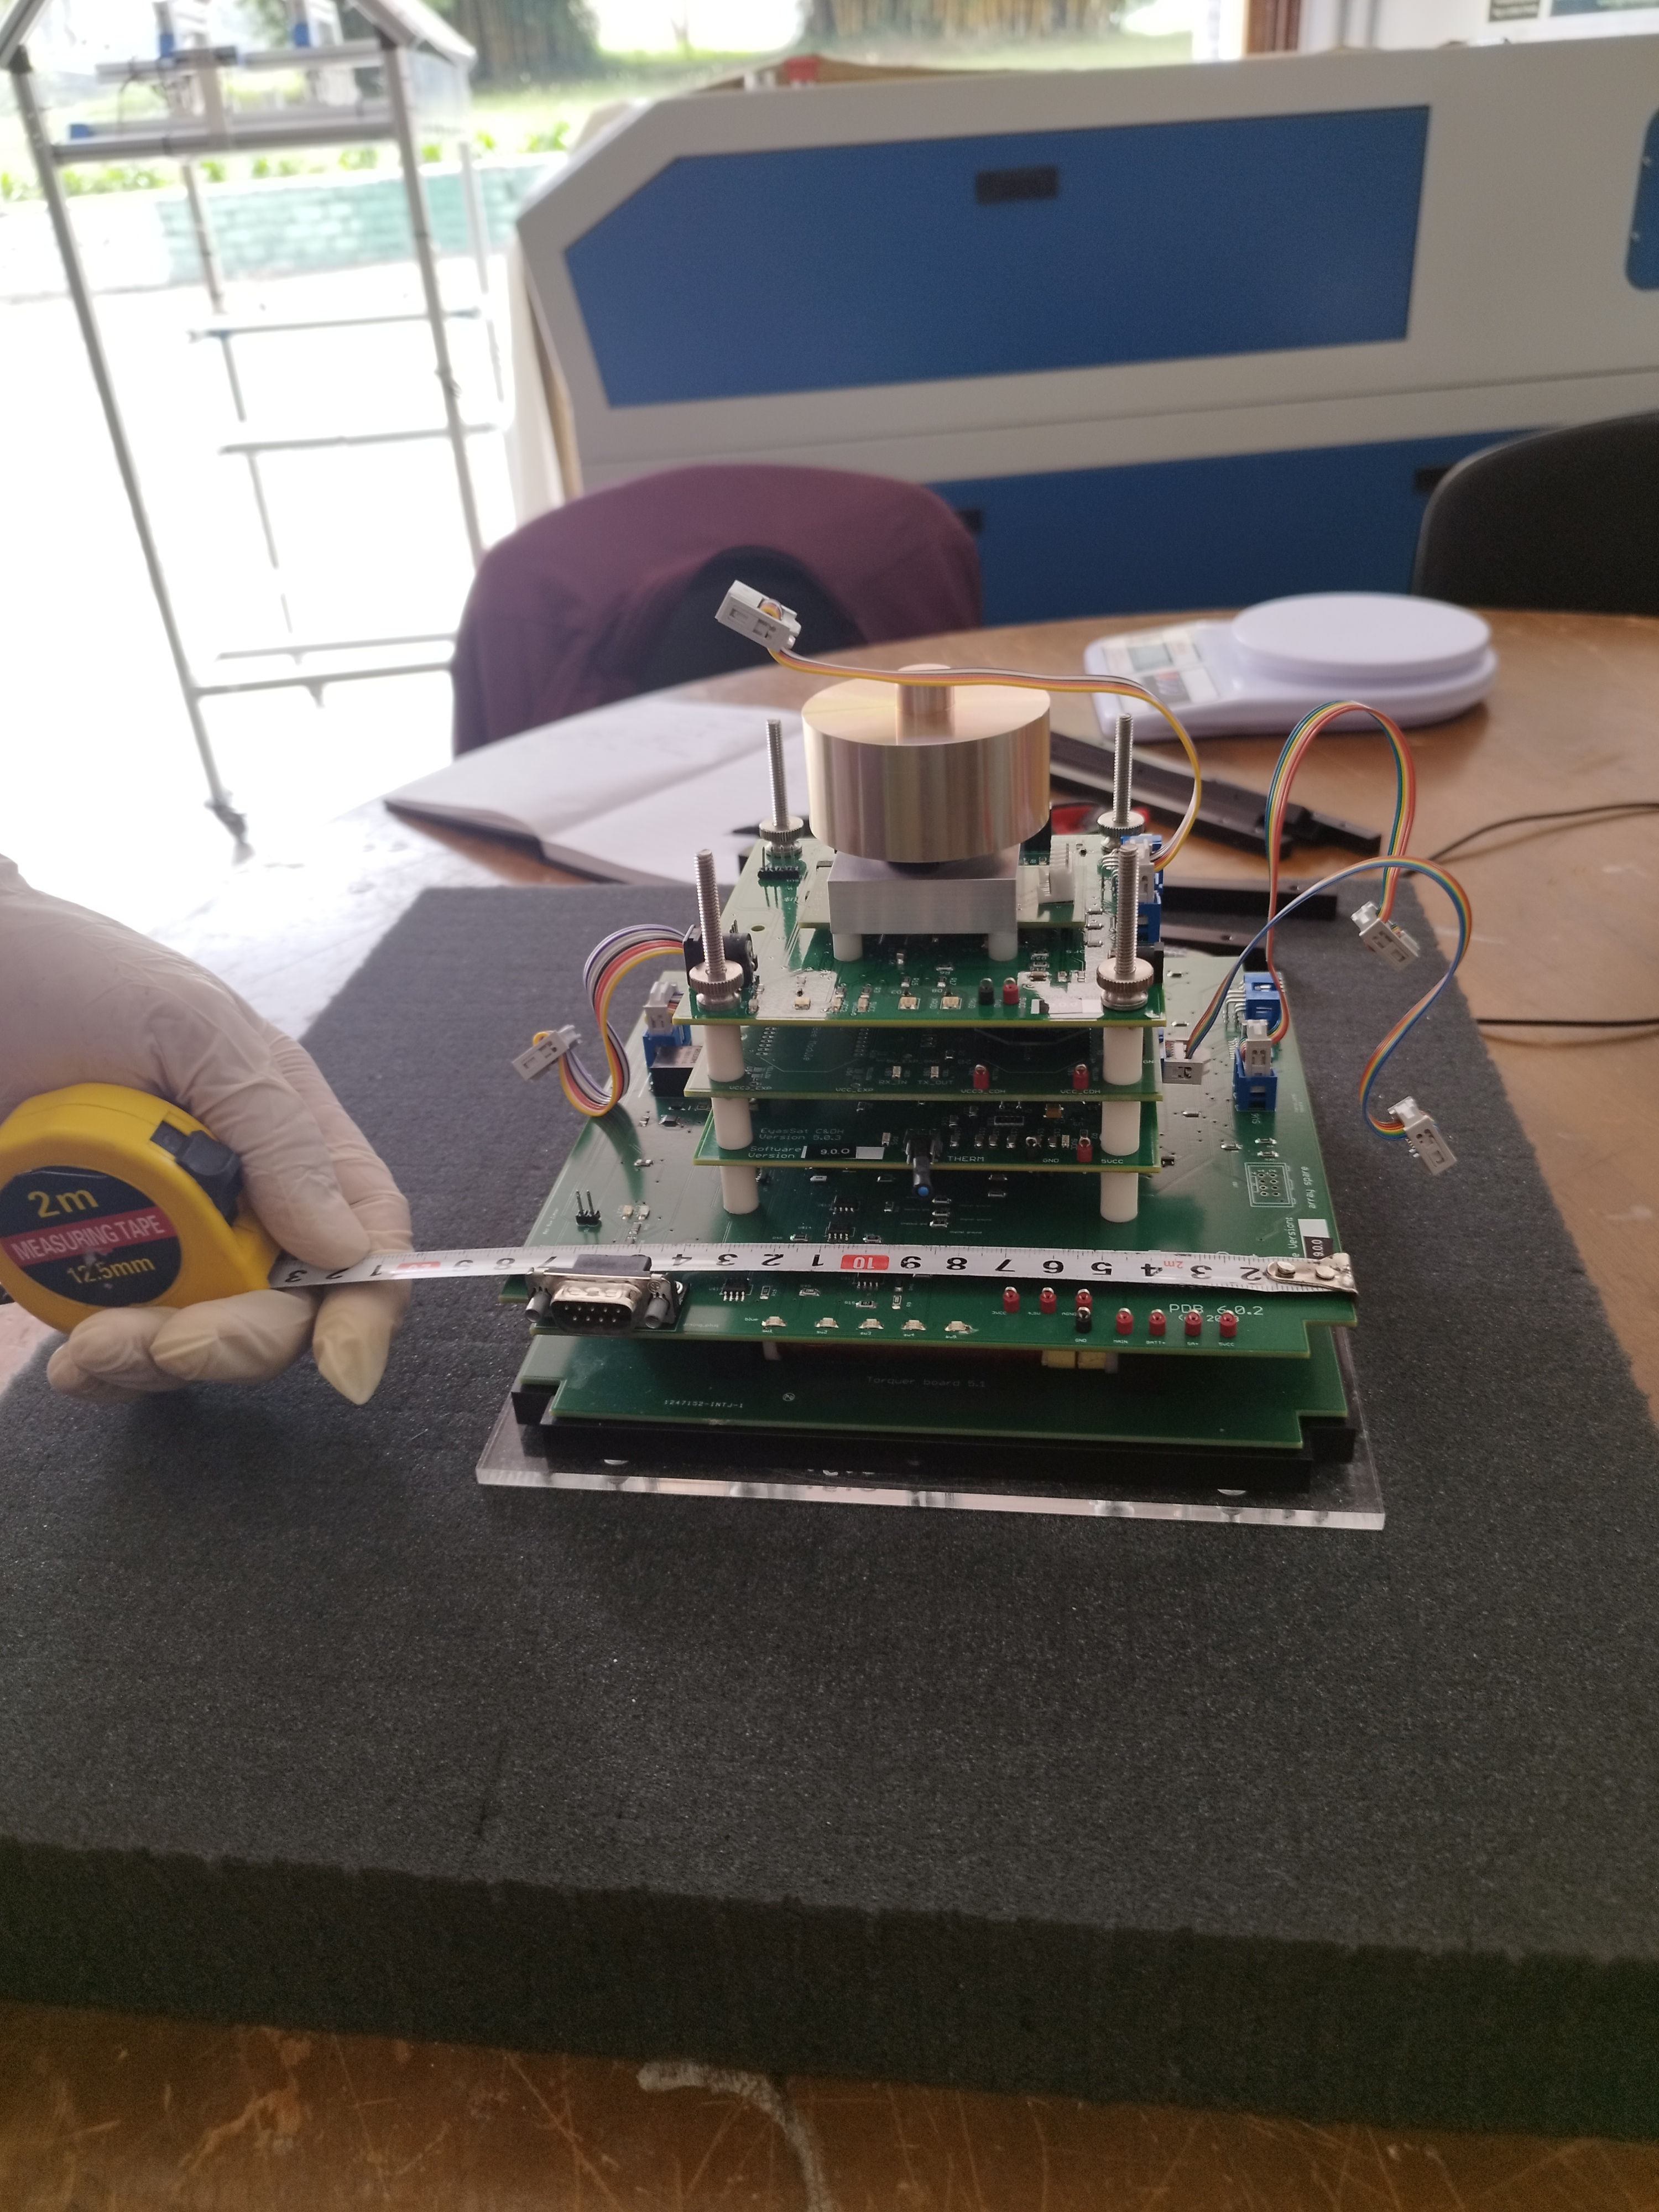
\includegraphics[width=0.31\textwidth]{imagenes/modelo_dinamico/eyassat_medicion.jpg}}
	\subfloat[Pesaje de la placa inferior del módulo ADCS.]{
		\label{fig:placa_cube}
		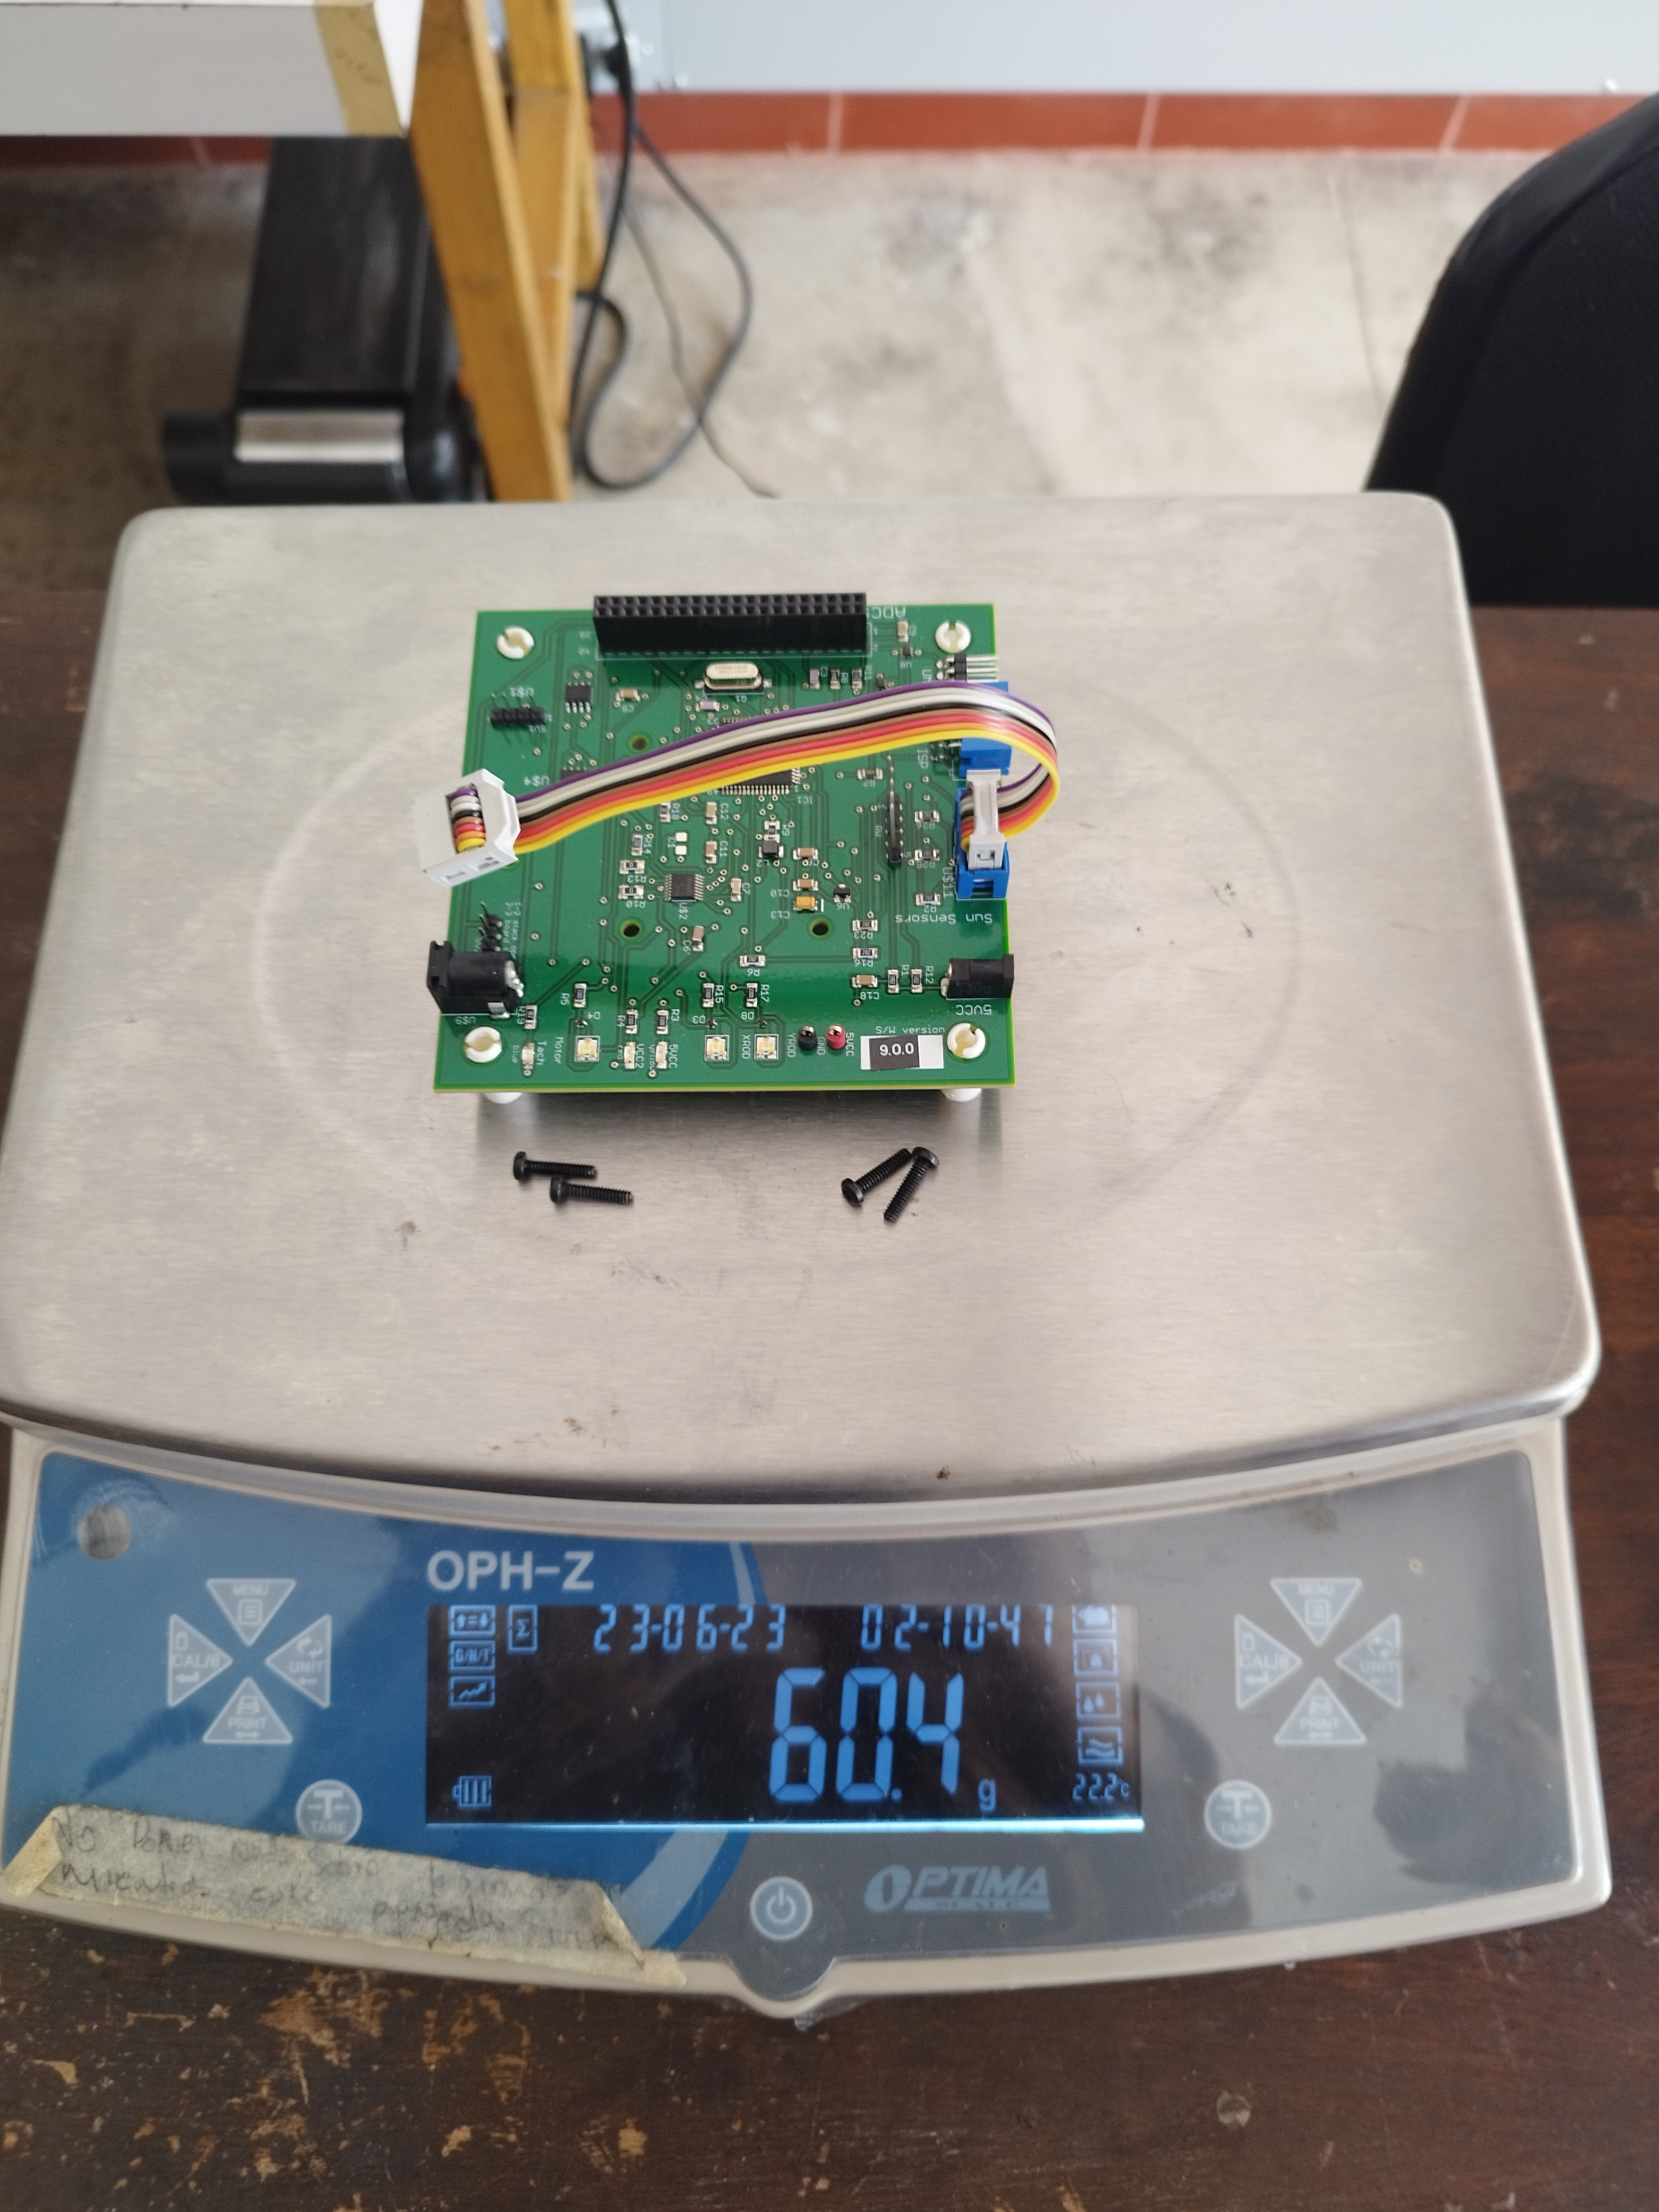
\includegraphics[width=0.31\textwidth]{imagenes/modelo_dinamico/placa_medicion.jpg}}
	
	\caption{Módulo ADCS del EyasSat}
	\label{fig:mediciones}
\end{figure}


\begin{figure}[h!]
	\begin{center}
		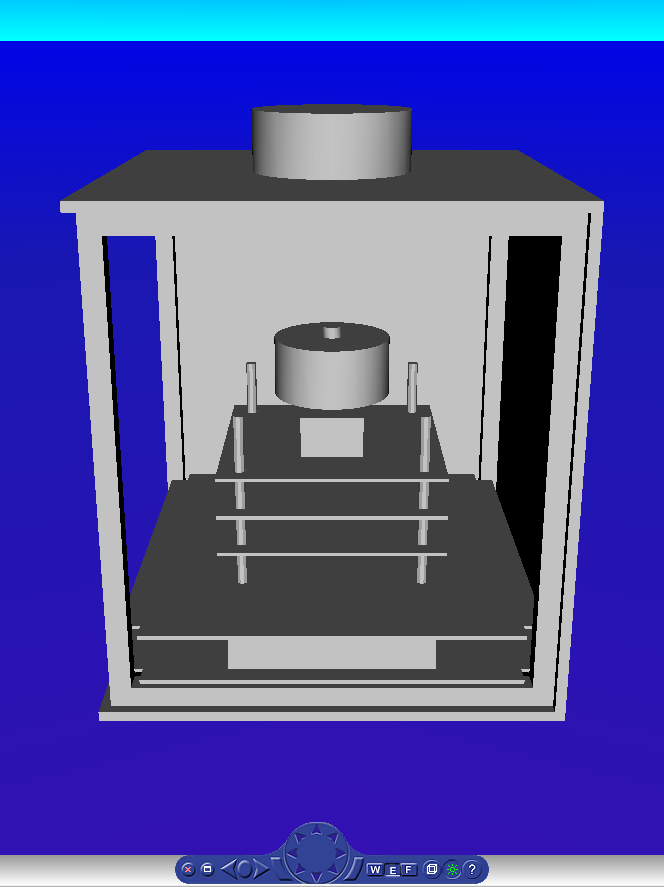
\includegraphics[scale=0.32]{imagenes/modelo_dinamico/escenario.PNG}\\
	\end{center}
	\caption{CAD del EyasSat en el entorno 3D World de Simulink.}
	\label{fig:escenario}
	\textit{}
\end{figure}
\newpage

\subsection{MODELADO DE PERTURBACIONES}

% Mencionar tipos de perturbaciones y el calculo de peor escenario para el Eyassat
Tal como se mencionó en la sección de ambiente espacial en LEO, las cuatro fuentes principales de perturbaciones son: 
\begin{itemize}
	\item Gradiente gravitacional.
	\item Aerodinámico. 
	\item Radiación solar.
	\item Campo geomagnético.
\end{itemize}

Dichas perturbaciones son representadas como fuerzas que actúan sobre el vehículo, sin embargo, cuando no actúan sobre el centro de masa, se producen torques externos que alteran la actitud y que deben ser tenidos en cuenta por el ADCS.

Existen algunos autores \cite{zapf2006robust}\cite{Andresen2005} que modelan las perturbaciones en función de la posición y actitud del vehículo a lo largo de su órbita. Sin embargo, para este trabajo se hizo una simplificación similar a la propuesta por P.S Bayod \cite{tes:Sorolla2019}, en la cual se parte de cada una de las ecuaciones de perturbaciones, extraídas de \cite{hughes2012spacecraft}, donde se evalúa el valor máximo de dicha perturbación. Como resultado, es posible sumar los torques externos como una constante, los cuales serán incluidos en la \textbf{eq. \ref{eq:modelo_dinamico}} del modelo dinámico.

\subsubsection{Torque Gravitacional}
\hfill \break
El torque gravitacional máximo puede ser expresado por:

\begin{equation}
T_g = \frac{3\mu_\mathTerra}{2R^3}\,\lvert I_{zz} -I_{yy}\,\rvert sin(2\theta)\label{eq:torque_grav}
\end{equation}

\noindent Donde:\\
$T_g$: es el torque gravitatorio máximo.\\
$\mu$: es el parámetro gravitatorio de la Tierra $(3,986$ $10^{14}$ $ m^3/s^2)$\\
$R$: es el radio de la órbita $(6370 + 500)$ $10^3$ $m$.\\
$\theta$: es la desviación máxima del eje $Z_o$ en el marco ORF.\\
$Izz, Iyy$: son los momentos de inercia sobre los ejes $Z_b$ e $Y_b$.\\

\noindent Tomando el valor máximo donde el torque actúa con un brazo a $45°$, entonces 
$$sin(2\theta) = 1$$
Por lo tanto, reemplazando los valores se obtiene que: 
$$T_g = 6.737\cdot10^{-9} Nm$$

\subsubsection{Torque Magnético}
\hfill \break
Similarmente a como lo expresa la \textbf{eq. \ref{eq:torque_mgt}}, el torque magnético generado por el satélite está dado por:

\begin{equation}
	T_m = \vec{m_{sat}}\times\vec{B}\label{eq:torque_mag}	
\end{equation}


\noindent Donde:\\
$\vec{m_{sat}}$ : es el dipolo residual del satélite.\\
$\vec{B}$: es la estimación del campo magnético terrestre para una órbita circular.\\

Debido a que el dipolo residual solo puede ser determinado experimentalmente, se tomará un valor de referencia de $0.01\,A $ $m^2$ usado en \cite{Giesselman2006}, donde desarrollan el cálculo  para un picosatélite similar al EyasSat.\\
Adicionalmente, el campo geomagnético puede ser estimado por:
\begin{equation}
	\vec{B} = \frac{2M}{R^3}\label{eq:campoMagnetico}
\end{equation}
Donde $M$ es el momento magnético terrestre ($M = 7.96\cdot10^{15}\:tesla\:m^3$) y el radio de la órbita $R$ es igual a $(6370 + 500)$ $10^3$ $m$. como en el cálculo anterior. Por consiguiente, el torque magnético es igual a:
$$T_m = 4.91\cdot10^{-7} Nm$$
	

\subsubsection{Torque Aerodinámico}
\hfill \break
La fuerza aerodinámica que experimenta el EyasSat, en una órbita determinada, debido a su interacción con la alta atmósfera puede ser expresada por:

\begin{equation}\label{eq:fuerza_aero}
	F_{aero} = \frac{1}{2}\rho\,V^2\,C_{d}\,A
\end{equation}

\noindent Donde:\\
$\rho$: es la densidad atmosférica\\
$V$: Velocidad del satélite \\
$C_d$: Coeficiente de arrastre $\approx$ 2.5.\\
$A$: Área superficial de incidencia $= \left(0.192\,m\right)^2$.\\
Para estimar la densidad del aire a 500 $km$ de altitud puede consultarse \cite{wertz2001mission} donde se obtiene que:
 $$\rho \approx 1.7\cdot10^{-11} kg/m^3$$
 Por otro lado, la velocidad lineal de un cuerpo que se encuentra en una órbita circular puede estimarse con la expresión:
 $$ V = \sqrt{\frac{GM}{R}} = \sqrt{\frac{6.67\,10^{-6}\times\,5.97\,10^{24}}{6370\,10^3 +500\,10^3}} =7613.27\,m/s $$

Finalmente, dado que la fuerza aerodinámica se aplica sobre el centro de presión, y éste tiene un desfase respecto al centro de masa, se genera un torque con un brazo equivalente a la distancia entre el C.G y el C.P. Por lo tanto, se tiene la expresión:

$$
\begin{aligned}
		& T_{aero} = F_{aero}\times\left(\overline{CP} - \overline{CG}\right)\\
		& T_{aero} = \frac{1}{2}\rho\,V^2\,C_{d}\,A\times\left(0.05\right) \\
		& T_{aero} =2.27\cdot10^{-6} Nm
\end{aligned}
$$		

 
\subsubsection{Torque por radiación solar}
\hfill \break
Para calcular esta perturbación se procede de manera similar respecto al torque aerodinámico. Primero se calcula la fuerza por radiación solar que se ejerce sobre el CubeSat, la cual viene dada por: 

\begin{equation}\label{eq:fuerza_radiacion}
	F_{SR} = -p_{SR}\,C_{R}\,A\,cos\,i	
\end{equation}

\noindent Donde:\\
$p_{SR}$: es la densidad fuerza de presión solar por unidad de área, la cual se calcula usando la densidad de flujo solar y la velocidad de la luz ($c$) con las siguientes expresiones: 

$$
\begin{aligned}
	& SF = 1.353\,W/m^2\\
	& p_{SR} = \frac{SF}{c} = \frac{1353}{3\cdot10^{8}}=4.51\cdot10^{-6}\,N/m^2	
\end{aligned}
$$
\\
\noindent$C_{R}$: es el coeficiente de reflectividad, el cual también puede ser expresado como: $C_R = 1+q$. De \cite{mcclain2001fundamentals} se obtiene un valor tipico de $q =0.6$ para satélites.\\
$i$: es el ángulo de incidencia del sol hacia la superficie del satélite.\\
$A$: es el área superficial del satélite $= \left(0.192\,m\right)^2$.\\
Dado que se busca obtener el peor escenario, el ángulo de incidencia será $i=0$, donde se maximiza la \textbf{eq. \ref{eq:fuerza_radiacion}}. En este sentido, una vez obtenida la ecuación de la fuerza de radiación, se calcula un torque a la misma distancia del centro de masas que en la sección anterior. Por lo tanto, se tiene que: 
 $$
 \begin{aligned}
 	& T_{SR} = F_{SR}\times\left(\overline{CP} - \overline{CG}\right)\\
 	& T_{SR} = p_{SR}\,C_{R}\,A\,cos\,i\times\left(0.05\right) \\
 	& T_{SR} =1.33\cdot10^{-8} Nm
 \end{aligned}
 $$
%\newpage
\subsubsection{Perturbaciones totales}
\hfill \break
Al recopilar y sumar las magnitudes de los torques de perturbación, como se evidencia en la \textbf{Tabla \ref{table:pertubaciones}}, se obtiene el torque total $T_{ext} = 2.78\cdot10^{-6}$. 

\begin{table}[h]
	\caption{\MakeUppercase{Torques externos de perturbación }}
	\begin{center}
		\begin{tabular}{ c c c}
			
			 &  \textbf{Perturbación} &  \textbf{Magnitud [Nm]}\\ \hline
			$T_g$ &  Torque Gravitacional & $6.73\cdot10^{-9}$ \\ 
			$T_m$ &  Torque Magnético & $4.91\cdot10^{-7}$ \\ 
			$T_{aero}$ &  Torque Aerodinámico & $2.27\cdot10^{-6}$ \\ 
			$T_{SR}$ &  Torque  Radiación Solar& $1.33\cdot10^{-8}$ \\ \hline
			\mbox{\boldmath$T_{ext}$} &  \textbf{Total}& \mbox{\boldmath$2.78\cdot10^{-6}$} \\
		\end{tabular}
	\end{center}
	\label{table:pertubaciones}
\end{table}

Dado que el problema solo contempla 1 grado de libertad en el eje Z, las perturbaciones se pueden escribir en notación vectorial como:

\begin{equation}\label{eq:torquePerturbacionVec}
	\mathbf{T_{ext}}=\left[\begin{array}{lll}
		0 & 0 & T_{ext}
	\end{array}\right]
\end{equation}

\subsection{MODELO DE RUEDAS DE REACCIÓN}

Como se mencionó en la sección del ADCS, las ruedas de reacción son motores de alta inercia. Por lo tanto, su modelamiento parte de un circuito de armadura para motores DC. El objetivo es obtener una expresión que relacione el voltaje de entrada con el torque de salida, es decir, determinar su función de transferencia. De igual forma, la corriente que consuma el motor también será un parámetro de utilidad para determinar los índices de desempeño de los controladores, por lo que es de interés obtener también su función de transferencia.
 
% Circuito de armadura
\begin{figure}[h]
	\begin{center}
		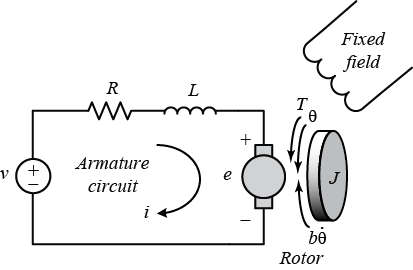
\includegraphics[scale=1.5]{imagenes/modelo_dinamico/motor.PNG}\\
	\end{center}
	\caption{Circuito de armadura de un motor DC.}
	\label{fig:motordc}
	\textit{}
\end{figure}

%Ecuacuiones 
A partir de la \textbf{Fig. \ref{fig:motordc}} puede realizarse un análisis de malla del circuito de armadura:

\begin{equation}\label{eq:armadura}
	L\frac{di(t)}{dt} =v(t) -Ri(t) -e(t)
\end{equation}

\noindent Donde:\\
 $e(t)$: es voltaje inducido en la armadura a través del flujo de campo fijo ("Fixed field").\\
 $R$: es la resistencia eléctrica.\\
 $L$: es la inductancia eléctrica.\\ 
 
 Por su parte, la ecuación mecánica del rotor viene dada por el modelo:

\begin{equation}\label{eq:torque_dc}
	J\frac{d\omega(t)}{dt} = T_{m}(t)-B\omega
\end{equation}

\noindent Donde:\\
$T_{m}(t)$: es el torque generado por el motor.\\
$J$: es el momento de inercia total del rotor y la carga.\\
$\omega$: es la velocidad angular del motor.\\ 
$B$: es el coeficiente de fricción.\\ 

Por otro lado, se asume que existe relación proporcional entre $e(t)$ y $\omega$ a través de la constante de campo $K_e$ \textbf{(eq. \ref{eq:constante_campo})}. Asi mismo, se supone una relación proporcional entre el torque mecánico y la corriente por medio de la constante de torque $K_t$ \textbf{(eq. \ref{eq:constante_torque})}

\begin{gather}
	e(t) = K_e\,\omega(t)\label{eq:constante_campo}\\[10pt]
	T_m(t) = K_t\,i(t)\label{eq:constante_torque}
\end{gather}

% eq y mostrar la eq de tranferencia de torque 
Finalmente, realizando la transformada de Laplace de las ecuaciones \textbf{(\ref{eq:armadura})} a \textbf{(\ref{eq:constante_torque})} se pueden obtener las funciones de transferencia para la corriente $i(s)$, $\omega(s)$ y el torque del motor $T_m(s)$ expresadas por. 

\begin{gather}
	\frac{T_m(s)}{v(s)}= \frac{K_t\left(Js+B\right)}{LJs^2 + \left(RJ+LB\right)s +RB+K_tK_e}\label{eq:trans_torque_voltaje}\\[10pt]	
	\frac{i(s)}{v(s)}= \frac{Js+B}{LJs^2 + \left(RJ+LB\right)s +RB+K_tK_e}\label{eq:trans_i_voltaje}\\[10pt]
	\frac{\omega(s)}{v(s)}= \frac{K_t}{LJs^2 + \left(RJ+LB\right)s +RB+K_tK_e}\label{eq:trans_omega_voltaje}
\end{gather}
\\
%Diagrama de bloques

En la \textbf{Fig. \ref{fig:bloquesRW}} se muestra la implementación del modelo de ruedas de reacción en Simulink. Ademas se calcular el torque y la corriente, dicho modelo calcula el momento angular $h_{RW}$ según la \textbf{eq (\ref{eq:torque_h})}.

\begin{figure}[h]
	\begin{center}
		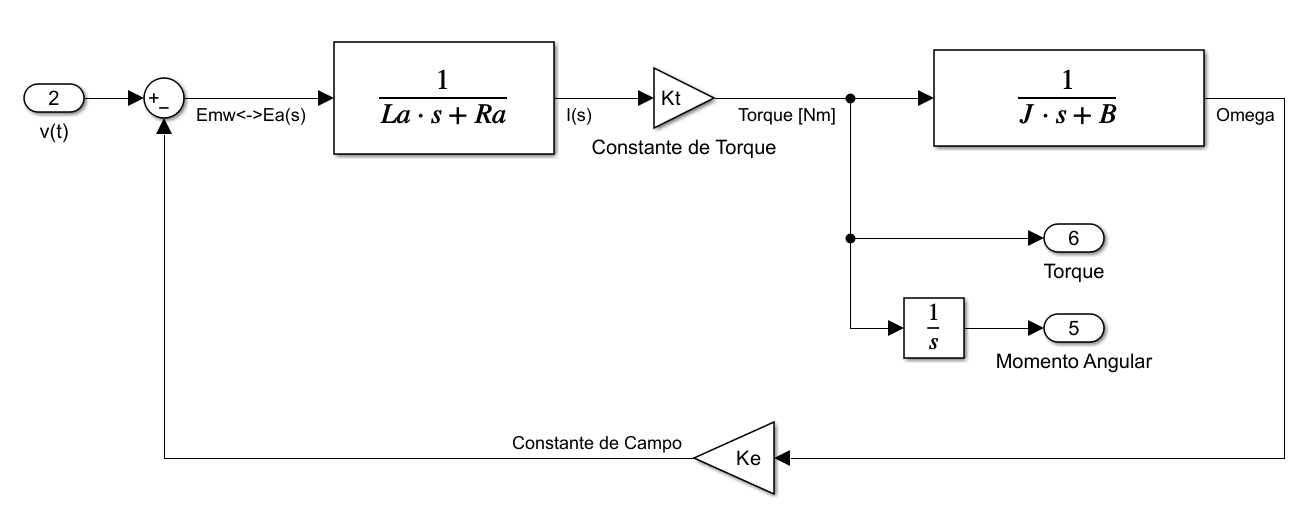
\includegraphics[scale=0.5]{imagenes/modelo_dinamico/bloquesRW.PNG}\\
	\end{center}
	\caption{Diagrama de bloques del modelo de RW en Simulink.}
	\label{fig:bloquesRW}
	\textit{}
\end{figure}

% Selección de referencia de RW y sus Parametros
Debido a que los manuales técnicos del EyasSat no especifican el modelo preciso del motor empleado para las RW. Se seleccionaron los parámetros electromecánicos del motor A-max 22 \textbf{(Fig. \ref{fig:motorRW})}, el cual fue empleado en el trabajo de Groenewald y Steyn \cite{Groenewald2014}. Dichos parámetros pueden se consultados en la \textbf{Tabla \ref{table:motorRW}}.


\begin{figure}[h]
	\begin{center}
		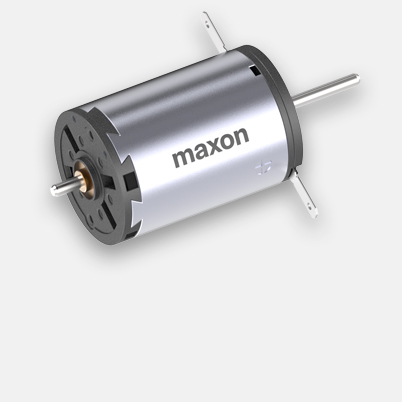
\includegraphics[scale=0.35]{imagenes/modelo_dinamico/motorRW.jpg}\\
	\end{center}
	\caption{Motor sin escobillas A-max 22.}
	\label{fig:motorRW}
	\footnotesize{Nota. Fuente \cite{maxon2023}}
\end{figure}

\begin{table}[!ht]
	\caption{\MakeUppercase{Parámetros electro-mecánicos RW }}
	\begin{center}
		\begin{tabular}{ c c c}
			
			&  \textbf{Parámetro} &  \textbf{Valor}\\ \hline
			$R$ &  Resistencia $(\Omega)$ & 3.36\\ 
			$L$ &  Inductancia $(mH)$ & 0.222\\ 
			$K_t$ &  Constante de torque $(Nm/A)$ & $8.55\cdot10^{-3}$ \\ 
			$K_e$ &  Constante de campo $(V/rad/s)$& $(1/1120)\cdot(60/2\pi)$ \\ 
			$B$ &  Coeficiente de fricción $(Nm/rad/s)$& $(1/438)\cdot(60/2\pi)\cdot10^{-3}$ \\
			$J$ &  Inercia total $(kg\,m^2)$& $7.157\cdot10^{-5}$ \\  
			$T_{max}$ & Torque máximo $(Nm)$ & $6.27\cdot10^{-3}$ \\
			$V_{max}$ & Voltaje máximo $(V)$ & $6$ \\
			$\omega_{max}$ & RPM máximas & $3940$ \\ \hline
		\end{tabular}
	\end{center}
	\label{table:motorRW}
\end{table}

\subsection{MODELO MAGNETORQUERS}
% Ecuacion/Diagrama de torque
Recordando la \textbf{eq (\ref{eq:torque_mgt})}, donde se tiene que $\vec{\tau} =\vec{M}\times\vec{B}$, el momento dipolar $\vec{M}$ puede expresarse como:

\begin{gather}
	\vec{M} = nIA\hat{n}\label{eq:momento_dipolar}\\[10pt]
	\vec{\tau} = nIA\,\hat{n}\times\vec{B}\label{eq:torque_mgt_completa}
\end{gather}

\noindent Donde:\\
$n$: es el número de vueltas de la bobina.\\
$I$: es la corriente que pasa por el magnetorquer.\\
$A$: es el área del magnetorquer en la dirección normal de la bobina. $\hat{n}$.

Tal como se muestra en la \textbf{Fig. \ref{fig:magnetorquers}a} , el momento dipolar tratará de alinearse con la resultante del campo magnético debido al torque generado, el cual es proporcional a la corriente, al numero de vueltas y al área como lo indica la \textbf{eq (\ref{eq:torque_mgt_completa})}.

La \textbf{Fig. \ref{fig:magnetorquers}b} muestra los actuadores reales del EyasSat, los cuales están dispuestos en los ejes $X$ e $Y$. Con el fin de determinar las propiedades mencionadas anteriormente, se realizaron mediciones de inductancia y resistencia como se muestra en la \textbf{Fig. \ref{fig:medicionH}}

\begin{figure}[h!]
	\centering
	\subfloat[Principio de funcionamiento de los magnetorquers.]{
		\label{fig:mgt_wp}
		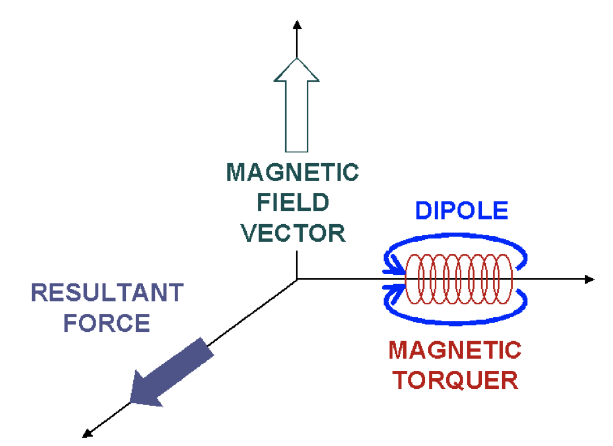
\includegraphics[width=0.5\textwidth]{imagenes/modelo_dinamico/magnetorquer.png}}
	\subfloat[Módulo de magnetorquers del EyasSat.]{
		\label{fig:mgt_real}
		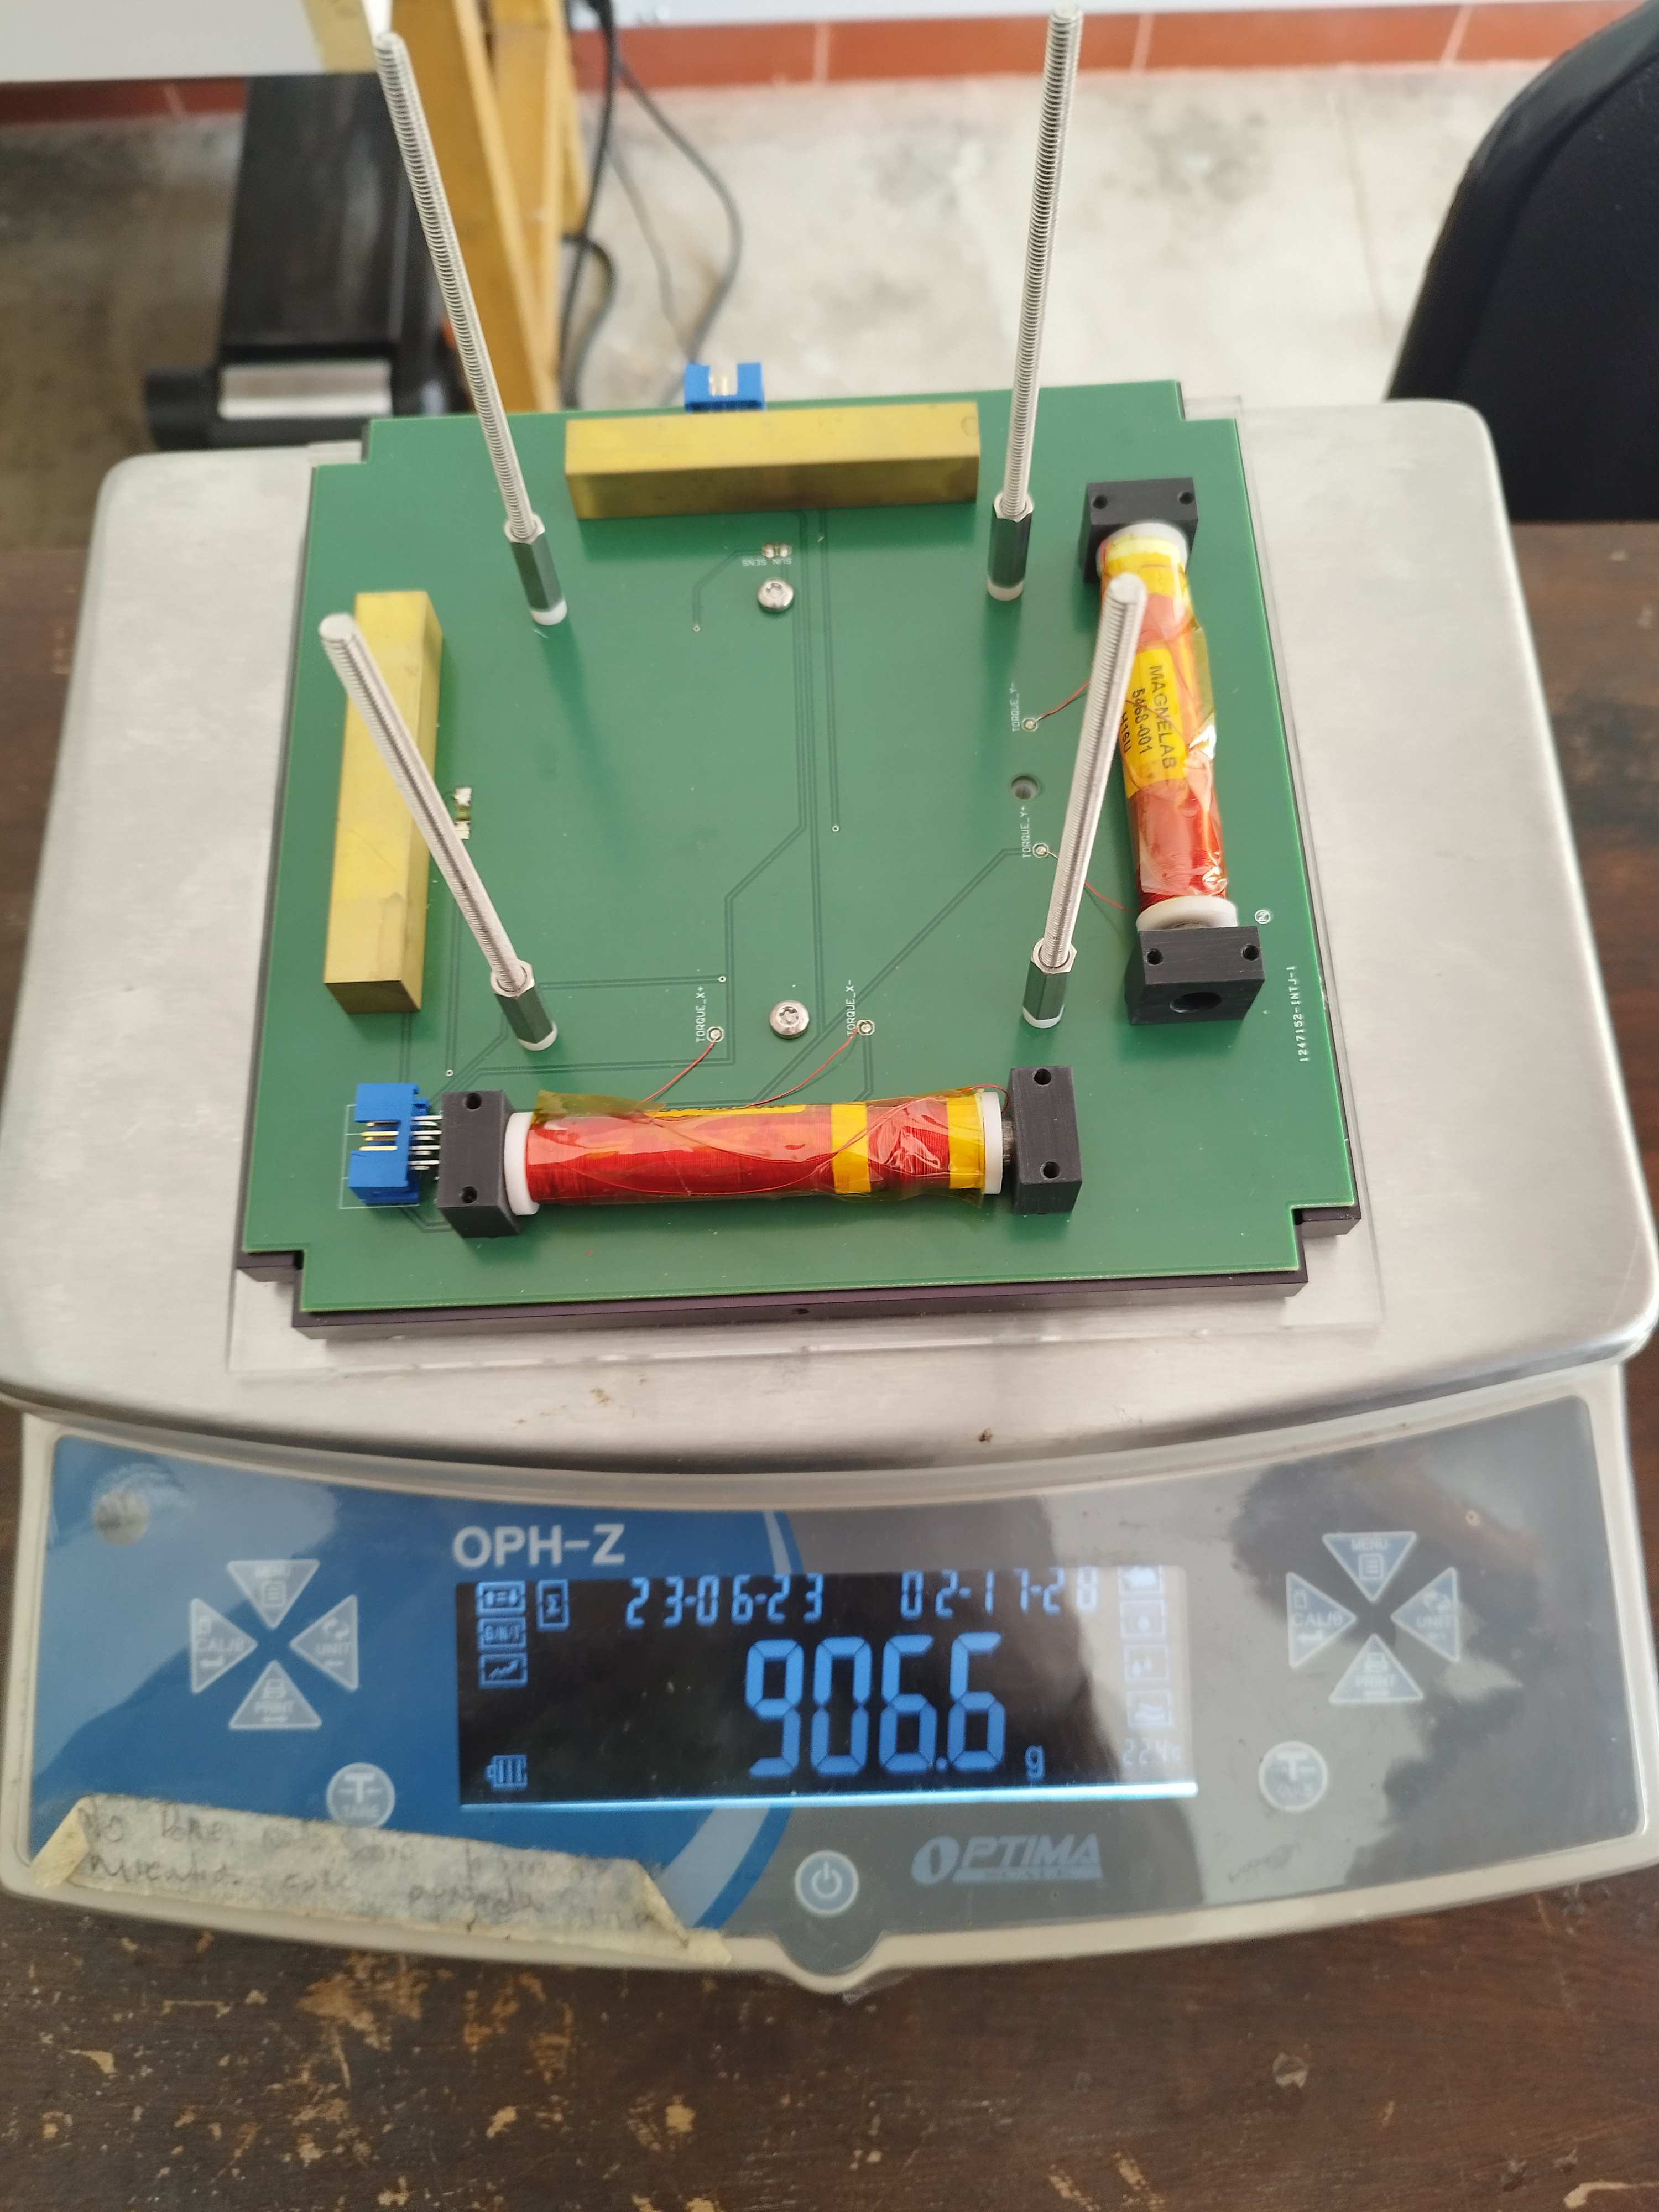
\includegraphics[width=0.31\textwidth]{imagenes/modelo_dinamico/magnetorquers.jpg}}
	
	\caption{Magnetorquers}
	\label{fig:magnetorquers}
\end{figure}

\begin{figure}[h]
	\begin{center}
		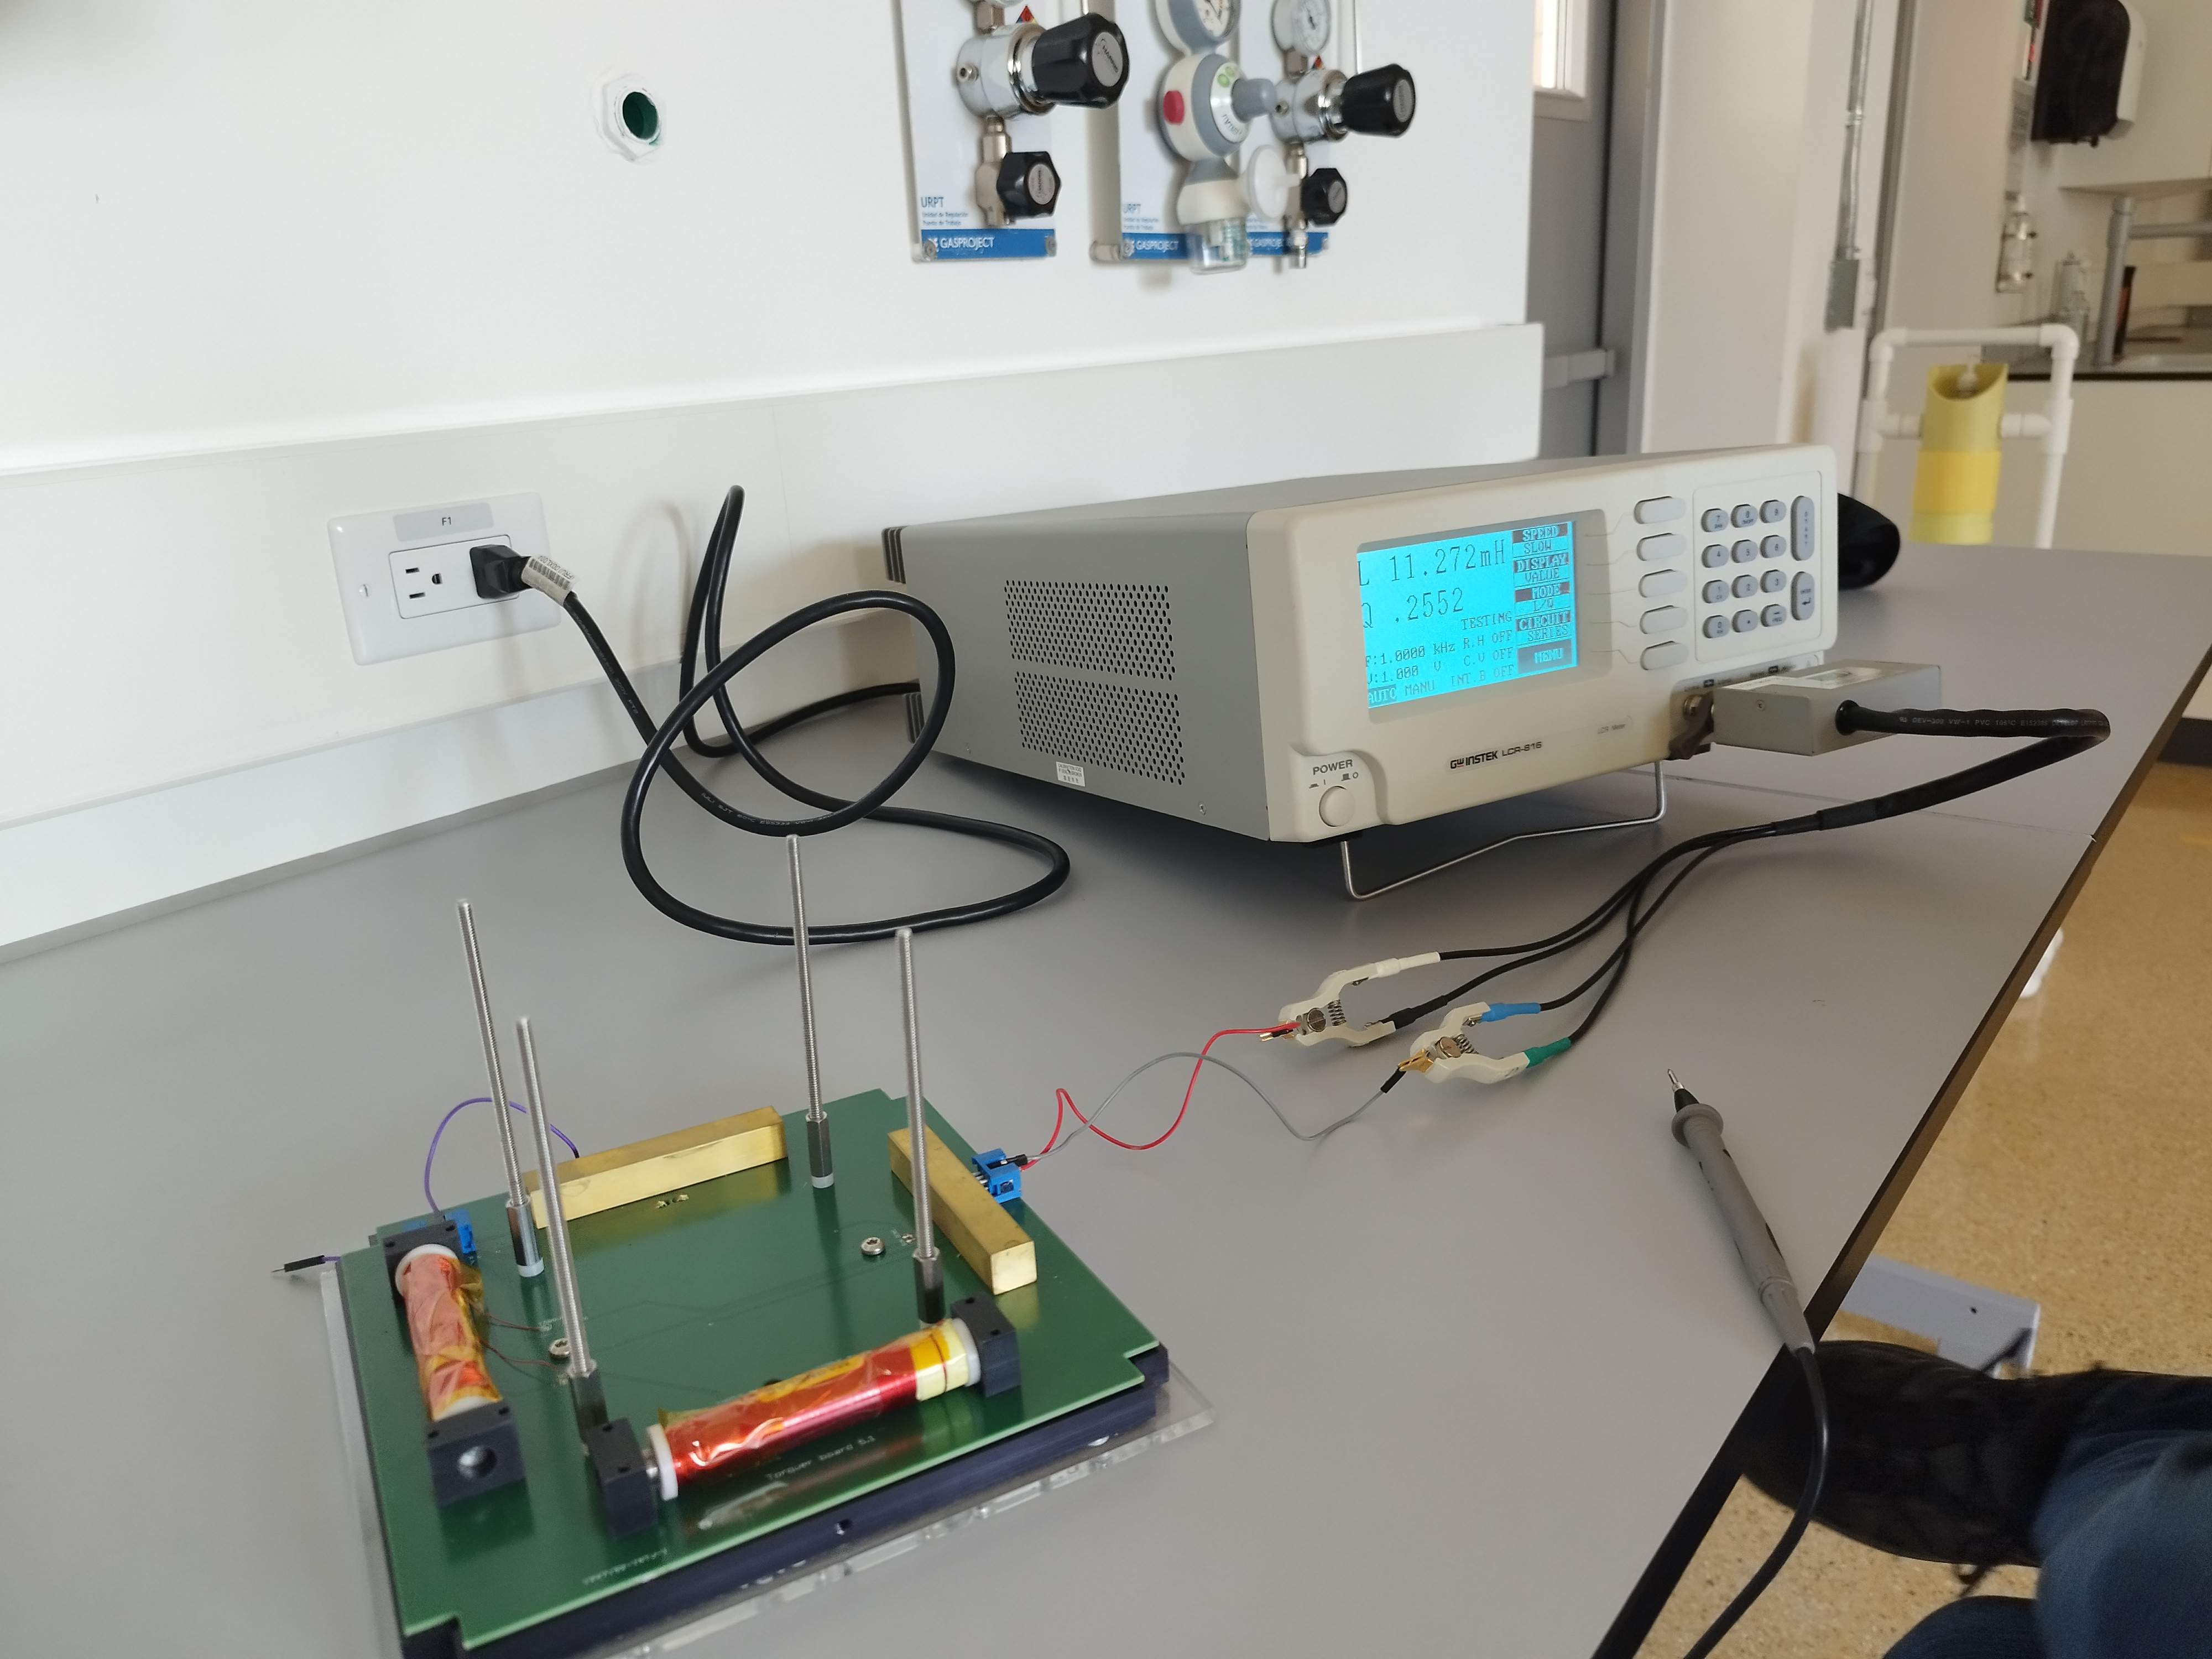
\includegraphics[scale=0.07]{imagenes/modelo_dinamico/medicion_mgt.jpg}\\
	\end{center}
	\caption{Medición de inductancia de magnetorquers.}
	\label{fig:medicionH}
	%	\footnotesize{Nota. Fuente \cite{maxon2023}}
\end{figure}

% Mostrar como se calcularon el numero de vueltas
No obstante, al comparar los parámetros con otros magnetorquers de usos similares, como el CubeTorquer, fabricado por la Universidad de Stellenbosh \cite{Groenewald2014}, éstos no correspondían con los valores de inductancia medidos, los cuales determinan el número de vueltas. Por lo tanto, se optó por determinar este parámetro usando las dimensiones de la bobina como se ve en la \textbf{Fig. \ref{fig:numVueltas}}:

\begin{gather}
	 N_{vueltas} = \#_{capas}\times \left(vueltas/capa\right)\label{key}\\[10pt]
	 N_{vueltas}= \left[\left(\diameter_{bobina}-\diameter_{nucleo}\right)/2\cdot \diameter_{cable} \right]\times L_{bobina} /\diameter_{cable}\\[10pt]
	 N_{vueltas}= 5412
\end{gather}

\begin{figure}[!ht]
	\begin{center}
		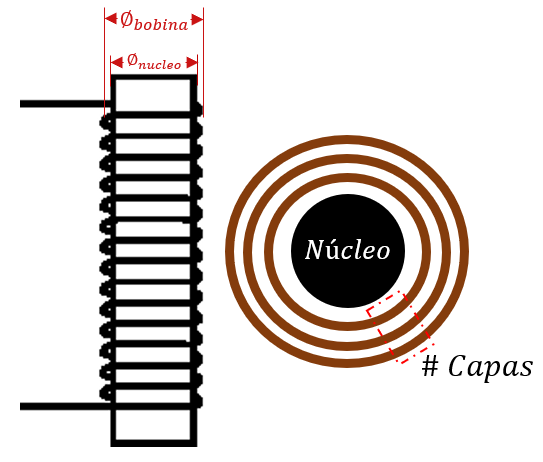
\includegraphics[scale=0.7]{imagenes/modelo_dinamico/dimensiones_mgt.png}\\
	\end{center}
	\caption{Cálculo de número de vueltas.}
	\label{fig:numVueltas}
	%	\footnotesize{Nota. Fuente \cite{maxon2023}}
\end{figure}

% Parametros de referencia
De esta manera, en la \textbf{Tabla \ref{table:Mgt}} se recopilaron los parámetros de los magnetorquers que se emplearían en el modelo. En la \textbf{Fig. \ref{fig:bloquesMgt}} se evidencia la implementación en Simulink para el magnetorquer $X$, la cual es igual para el $Y$. 
\newpage
\begin{table}[!ht]
	\caption{\MakeUppercase{Parámetros Magnetorquers }}
	\begin{center}
		\begin{tabular}{ c c c}
			
			&  \textbf{Parámetro} &  \textbf{Valor}\\ \hline
			$\vec{M}$ &  Momento magnético nominal $(Am^2)$ & 0.2834\\ 
			$T_{max}$ &  Torque máximo $(Nm)$ & $1.843\cdot10^{-5}$ \\ 
			$R$ &  Resistencia $(\Omega)$& $30$ \\ 
			$\diameter_{b}$ &  Diámetro bobina $(cm)$& $2$ \\
			$\diameter_{c}$ &  Diámetro núcleo $(cm)$& $0.77$ \\
			$\diameter_{w}$ &  Calibre cable $(cm)$& $0.03$ \\  
			$L_{b}$ & Longitud bobina $(cm)$ & $7.92$ \\
			$N_{b}$ & Número de vueltas de bobina  & $5412$ \\
			$L$ & Inductancia $(H)$ & $0.585$ \\ \hline
			
		\end{tabular}
	\end{center}
	\label{table:Mgt}
\end{table}


% Diagrama de bloques

\begin{figure}[h]
	\begin{center}
		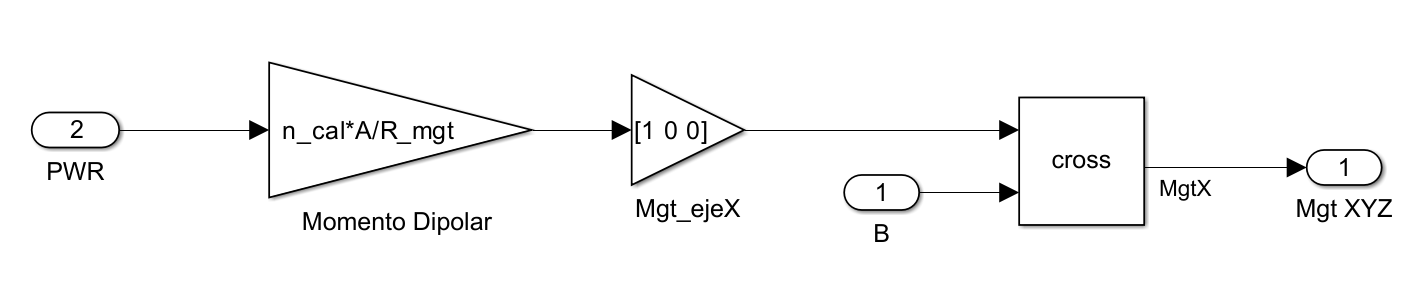
\includegraphics[scale=0.4]{imagenes/modelo_dinamico/bloquesMgt.PNG}\\
	\end{center}
	\caption{Diagrama de bloques Magnetorquer X.}
	\label{fig:bloquesMgt}
	\textit{}
\end{figure}


\subsection{MODELO DE CAMPO MAGNÉTICO}

Con el fin de evaluar el desempeño de los magnetorquers en diferentes órbitas se requiere determinar la magnitud del campo magnético a lo largo de la trayectoria del EyasSat. Para ello se recurre a un script de Matlab encargado de calcular todas las intensidades de campo para luego ser leídas por el modelo en Simulink.

\begin{figure}[!ht]
	\begin{center}
		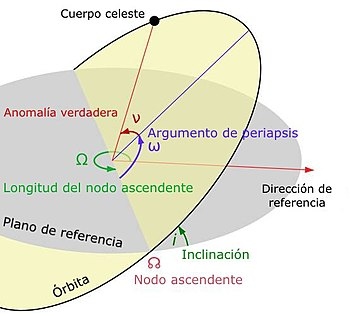
\includegraphics[scale=0.6]{imagenes/modelo_dinamico/Elementos_orbitales.jpg}\\
	\end{center}
	\caption{Elementos orbitales.}
	\label{fig:elementosOrbitales}
	\textit{}
\end{figure}
	 
La lógica de este procedimiento se ilustra en el diagrama de flujo de la \textbf{Fig. \ref{fig:flujoCampo}}, el cual inicia definiendo los parámetros orbitales, mostrados en la \textbf{Fig. \ref{fig:elementosOrbitales}}, donde:

\noindent$RAAN$: ascensión recta del nodo ascendente.  \\
$\omega$: argumento de perigeo. \\
$\nu$: anomalía verdadera\\
$i$: inclinación \\
$a$: semi-eje mayor \\
$e$: excentricidad.
	 
% Diagrama de flujo : 
Posteriormente, estos parámetros son usados por el propagador para determinar las coordenadas $XYZ$ de la órbita, en el marco $ECI$. Luego estas coordenadas son convertidas en latitud, longitud y altura ya que la función \textit{igrfmagm} de Matlab recibe estos parámetros de entrada. Dicha función se encarga de calcular las intensidades de campo para cada punto de la órbita, sin embargo, estas intensidades en encuentran en el marco LVLH.
\begin{figure}[!ht]
	\begin{center}
		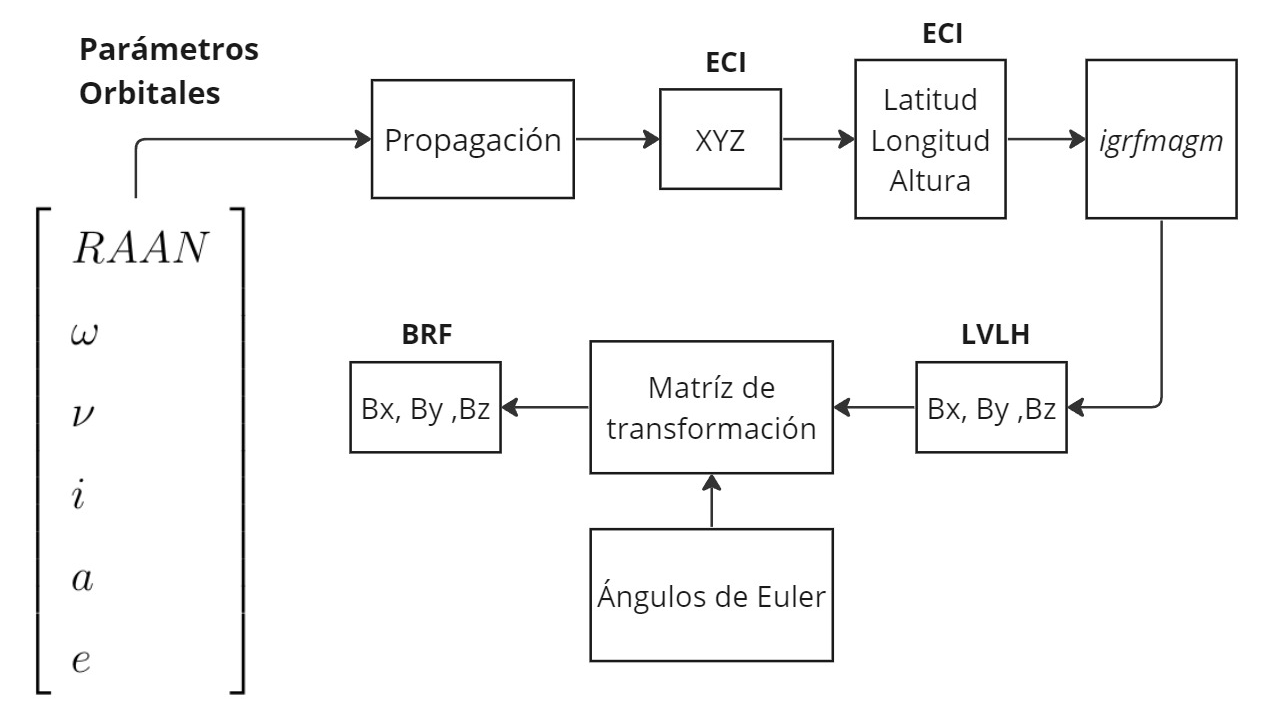
\includegraphics[scale=0.4]{imagenes/modelo_dinamico/flujo_campo.png}\\
	\end{center}
	\caption{Diagrama de flujo para cálculo de intensidades de campo para una órbita determinada.}
	\label{fig:flujoCampo}
	\textit{}
\end{figure}
% 4. Transformacion de coordenadas NED a BRF 
Hasta este punto, los pasos anteriores se realizan en Matlab con el fin de ahorrar capacidad de computo y disminuir los tiempos de simulación. Sin embargo, para poder transformar las intensidades de campo del marco LVLH/NED al marco BRF se requiere conocer los ángulos de Euler ($RPY$) en cada punto de la órbita. Por tal motivo, la implementación de Simulink  \textbf{(Fig. \ref{fig:modeloB})}  recibe el vector de campos magnéticos LVLH y realiza la transformación de marcos de referencia usando la actitud instantánea del satélite.

% Diagrama de bloques 

\begin{figure}[!ht]
	\begin{center}
		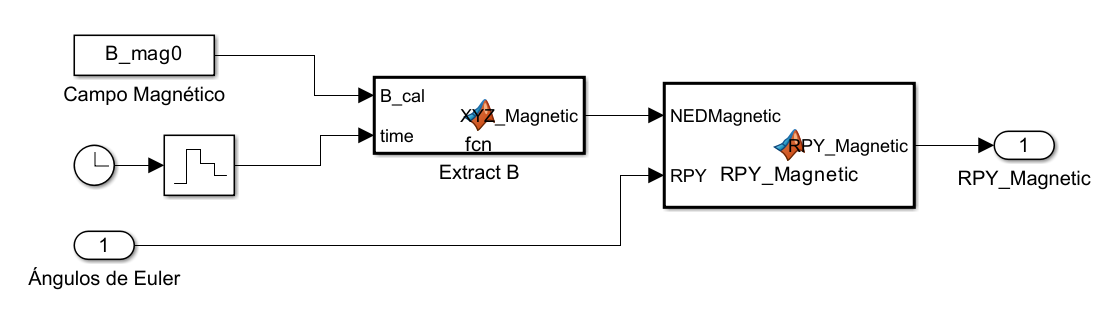
\includegraphics[scale=0.4]{imagenes/modelo_dinamico/modelo_campoMagnetico.PNG}\\
	\end{center}
	\caption{Implementación del modelo de campo geomagnético en Simulink.}
	\label{fig:modeloB}
	\textit{}
\end{figure}

La transformación de de intensidades de campo magnético está dada por: 
\begin{equation}	
	\left[\begin{array}{c}
		B_x\\
		B_y\\
		B_z
	\end{array}\right]_{BRF} = 
	C_{BRF}^{NED}
	\left[\begin{array}{c}
		B_x\\
		B_y\\
		B_z
	\end{array}\right]_{NED}	
\end{equation}

Para hallar la matriz $C_{BRF}^{NED}$, se remite a \cite{grewal2007global} donde se define la matriz:

$$
C_{ENU}^{BRF}=\left[\begin{array}{ccc}
	S_Y C_P & C_R C_Y+S_R S_Y S_P & -S_R C_Y+C_R S_Y S_P \\
	C_Y C_P & -C_R S_Y+S_R C_Y S_P & S_R S_Y+C_R C_Y S_P \\
	S_P & -S_R C_P & -C_R C_P
\end{array}\right],
$$
Donde :
$$
\begin{aligned}
	S_R & =\sin (R), \\
	C_R & =\cos (R), \\
	S_P & =\sin (P), \\
	C_P & =\cos (P), \\
	S_Y & =\sin (Y), \\
	C_Y & =\cos (Y),
\end{aligned}
$$

Por otro lado, se conoce la transformación del marco $NED$ al $ENU$ :
$$
C_{ENU}^{NED}=\left[\begin{array}{ccc}
	0 &1 &0 \\
	1 & 0 & 0 \\
	0 & 0 &-1
\end{array}\right]
$$

Finalmente, usando las propiedades \textbf{(\ref{eq:transformada1})} y \textbf{(\ref{eq:transformada2})}, descritas en la sección de transformación de marcos de referencia, se tiene que:

\begin{gather}
	C_{BRF}^{NED} = \left(C_{ENU}^{BRF}\right)^T\,C_{ENU}^{NED}\\[10pt]
	C_{BRF}^{NED} = C_{BRF}^{ENU}\,C_{ENU}^{NED}
\end{gather}
	


%\begin{figure}[!ht]
%	\begin{center}
%		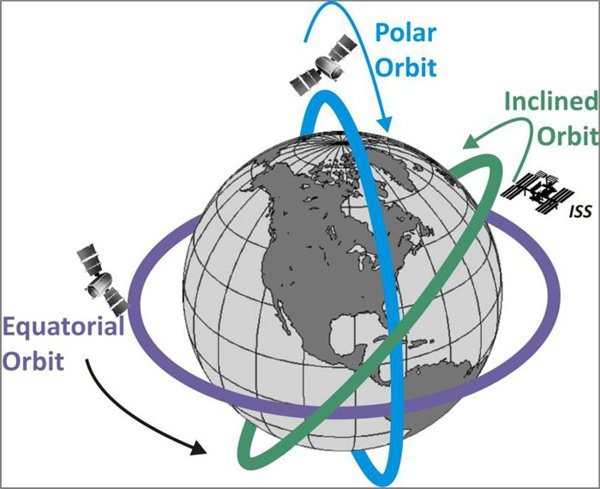
\includegraphics[scale=0.3]{imagenes/analisis_de_orbitas/orbitas.jpg}\\
%	\end{center}
%	\caption{Orbitas a evaluar}
%	\label{fig:orbitas}
%	\textit{}
%\end{figure}

\newpage
\section{DISEÑO CONTROLADORES}

Tal como se mencionó en el planteamiento del problema, las estrategias de control tienen como objetivos desaturar las RW a la vez que permiten que el EyasSat alcance una actitud determinada ante diferentes respuestas. En cuanto al control de actitud se diseñaron dos controladores, PID y LQR, los cuales determinan el voltaje que  debe suministrar el subsistema de potencia a las RW. Por otro lado, la desaturación se logra por medio de la acción de control de los magnetorquers, la cual se rige por dos métodos diferentes dependiendo del controlador de actitud:

\begin{itemize}
	 \item Tanto para el controlador PID y LQR, se evalúa una ley de control para desaturación que define el torque del actuador dado por la siguiente expresión:
	 	\begin{equation}\label{eq:ley_de_control_sat}
	 		\vec{\tau}_{mgt} = k\Delta h =\vec{M}\times\vec{B} 
	 	\end{equation} 
	 Donde $k$ es la ganancia para el control de desaturación y $\Delta h$ es la diferencia entre el momento angular del satélite y el momento angular de las RW. La representación simplificada de este lazo de control puede evidenciarse en la \textbf{Fig. \ref{fig:desaturacionDiagrama}}.
	 
	 \begin{figure}[!ht]
	 	\begin{center}
	 		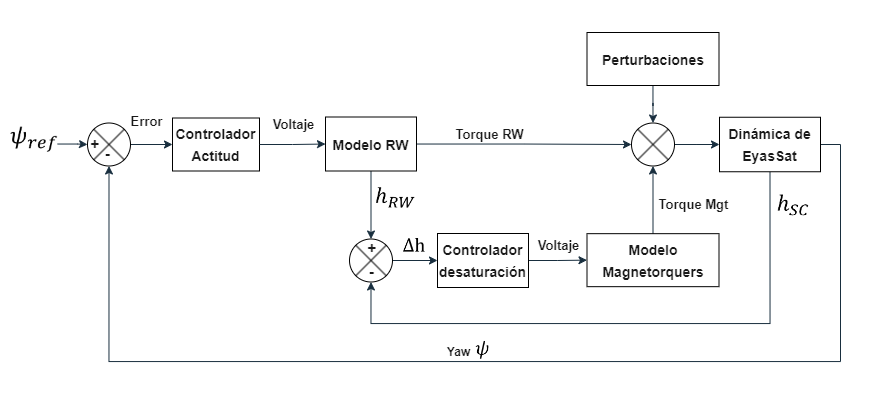
\includegraphics[scale=0.55]{imagenes/controladores/Diagrama_controlador.PNG}\\
	 	\end{center}
	 	\caption{Control de lazo cerrado para el control de actitud y ley de control de saturación.}
	 	\label{fig:desaturacionDiagrama}	 	
	 \end{figure}
	 
	 \item Para el LQR, se implementa un controlador en cascada que recibe los valores de referencia calculados a partir de las ganancias de la matriz $K$. Este lazo de control de ilustra en la \textbf{Fig. \ref{fig:desaturacionDiagrama2}}. El diseño de los controladores y la definición del espacio de estados serán desarrollados en la siguiente subsección.  
	 
	 \begin{figure}[!ht]
	 	\begin{center}
	 		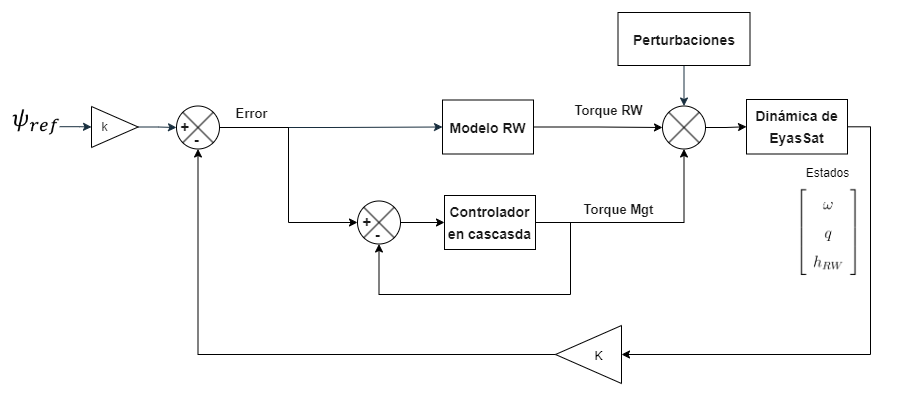
\includegraphics[scale=0.55]{imagenes/controladores/Diagrama_controlador2.PNG}\\
	 	\end{center}
	 	\caption{Control de lazo cerrado para el control de actitud y controlador en cascada.}
	 	\label{fig:desaturacionDiagrama2}	 	
	 \end{figure} 	  
\end{itemize}



\subsubsection{Linealización y Espacio de Estados}
\hfill \break
Las ecuaciones dinámicas \textbf{(\ref{eq:modelo_dinamico})} y cinemáticas \textbf{(\ref{eq:modelo_cinematico})} conforman el espacio de estados que se evidencia en 
\textbf{(\ref{eq:espacio_estados_non})}, donde $x$ son los estados definidos por la velocidad angular ($w$), cuaterniones ($q$) y el momento angular de las RW ($h_w$). 
%Sistema no lineal 

\begin{equation}\label{eq:espacio_estados_non}
	\begin{aligned}
		& \underbrace{\left[\begin{array}{c}
				\dot{\omega} \\
				\dot{q} \\
				\dot{h_{w}}
			\end{array}\right]}_{\dot{x}}=\underbrace{\left[\begin{array}{c}
				{\mathrm{I}}^{-1}\left(T_{\mathrm{ext}}+T_{c}-{\mathrm{S}}(\omega)\left({\mathrm{I}} \omega_{b}+h_{\mathrm{w}}\right)\right) \\
				\frac{1}{2} {\Omega} q \\
				T_{RW}
			\end{array}\right]}_{f(x,u)}\\[10pt]
		& \underbrace{\left[\begin{array}{c}
				\omega \\
				q \\
				h_{w}
			\end{array}\right]}_y=\underbrace{\left[\begin{array}{ccc}
				\underline{1}_{3 \times 3} & \underline{0}_{3 \times 4} & \underline{0}_{3 \times 3}\\
				\underline{0}_{4 \times 3} & \underline{1}_{4 \times 4} & \underline{0}_{4 \times 3} \\
				\underline{0}_{3 \times 3} & \underline{0}_{3 \times 4} & \underline{1}_{3 \times 3}
			\end{array}\right]}_{{\mathrm{C}}} \underbrace{\left[\begin{array}{c}
				\omega \\
				q \\
				h_{w}
			\end{array}\right]}_x
	\end{aligned}	
\end{equation}

% Linealizacion
Sin embargo, la naturaleza de las ecuaciones de $f(x,u)$ es no lineal. Por lo tanto, con el fin de diseñar los controladores, estas ecuaciones deben ser linealizadas sobre un punto de control ($\bar{\omega},\bar{q},\bar{h_w}$) donde se tienen en cuenta pequeñas variaciones sobre ese punto representados por el símbolo $\sim$ sobre los estados. En este sentido, los estados y las entradas del sistema se expresan de la forma: 

\begin{equation}
	\begin{aligned}
		& x(t) =\bar{x}(t)+ \tilde{x}(t) \\
		& u(t) =\bar{u}(t)+ \tilde{u}(t) 		
	\end{aligned}
\end{equation}	

No obstante, debe hacerse una distinción entre las entradas, las cuales corresponden a los torques que afectan la dinámica del sistema. El torque de control $T_c$ está definido por la contribución de los torques generados por las RW y los magnetorquers:
$$ T_c = T_{RW} +T_{mgt}$$
Por otro lado, los torques externos no se consideran entradas ya que son perturbaciones a las que no se les ejerce control. Por lo tanto, son tratados en el término $u_d$. De esta manera, es posible expresar el espacio de estados de la siguiente forma:
 
\begin{equation}\label{eq:espacio_de_estados}
	\begin{aligned}
		& \dot{x}(t) =\mathrm{A}x(t)+ \mathrm{B}u(t)+ \Gamma u_d(t)
%		& y(t) =\mathrm{C}x(t)+ \mathrm{D}y(t)		
	\end{aligned}
\end{equation}	
\noindent Donde: 
\begin{equation}\label{eq:estados_y_entradas}
	\begin{aligned}
		& x(t) = \left[\begin{array}{c}
			\omega \\
			q \\
			h_{w}
		\end{array}\right];
		& u(t) = \left[\begin{array}{c}
			T_{RW} \\
			T_{mgt}
		\end{array}\right]; 
		&\;u_d(t) = \left[\begin{array}{c}
			T_{ext} \\		
		\end{array}\right]		
	\end{aligned}
\end{equation}

\begin{equation}
	\begin{aligned}		
		&\mathrm{A}_{ij}= \frac{\partial f_i}{\partial x_j};	
		&\mathrm{B}_{ij}= \frac{\partial f_i}{\partial u_j};	
		&\;\Gamma_{ij}= \frac{\partial f_i}{\partial u_{d_j}}		
	\end{aligned}
\end{equation}
Con el fin de hallar las matrices $A$, $B$ y $\Gamma$ debe determinarse una expresión linealizada para los términos de $f(x,u)$, constituidos por las ecuaciones dinámicas y cinemáticas.

\paragraph{Linealiazión de la ecuación dinámica}
\hfill \break
Según el procedimiento planteado en \cite{Andresen2005}, se parte de la ecuación dinámica \textbf{(\ref{eq:modelo_dinamico})} :
$$
 \dot{\omega_b}=I^{-1}\left[-S(\omega)\left(I \omega_b+h_w\right)+T_{ext}+T_c\right]
$$

y se escoge un punto de operación $\bar{\omega}$ para el sistema y se modela con pequeñas variaciones $\tilde{\omega}$ en dicho punto de operación. Esto se expresa en:
\begin{equation}
	\begin{aligned}
		& \omega = \omega(t+\Delta t) = \bar{\omega} + \tilde{\omega}\\
		& \dot{\omega} = \tilde{\omega}
	\end{aligned}	 
\end{equation}

Tomando la \textbf{eq. (\ref{eq:modelo_dinamico})} es posible considerar $T_{ext}$ como una constante al rededor del punto de control de un marco de tiempo $\Delta t$. Por lo tanto, $\dot{\omega}$ se puede expresar como una función de $\omega$, $T_c$ y $h_w$. De esta manera, es posible linealizar usando la expansión de Taylor de primer orden, obteniendo la siguiente expresión:

\begin{equation}\label{eq:modelo_dinamico_linealizado}
	\dot{\omega_b}=I^{-1}\left[S(I\bar{\omega}-S(\bar{\omega})I+S(\bar{h_w})\right]\tilde{\omega}-I^{-1}S(\bar{\omega})\tilde{h_w}+I^{-1}\left(T_{RW}+T_{mgt}\right)
\end{equation}

\paragraph{Linealiazión de la ecuación cinemática}
\hfill \break
Siguiendo un procedimiento similar al anterior, se tiene que $dq$ es la orientación en el tiempo $t +\Delta t$ relativa a la actitud en el tiempo $t$, por lo tanto $\tilde{q}$ se puede expresar como:
 
\begin{equation}
	\begin{aligned}		
		& \tilde{q} = \left[\begin{array}{c}				
				\tilde{\epsilon_1}\\
				\tilde{\epsilon_2}\\
				\tilde{\epsilon_3} \\
				\tilde{\eta}
			\end{array}\right] =
			\left[\begin{array}{c}
				\tilde{g}\\				
				\tilde{q_4}
			\end{array}\right] =
				\left[\begin{array}{c}
				dq_1\\				
				dq_2\\
				dq_3\\
				dq_4
			\end{array}\right] =
				\left[\begin{array}{c}
					e_x sin\left(\frac{1}{2}\omega dt\right)\\
					e_y sin\left(\frac{1}{2}\omega dt\right)\\
					e_z sin\left(\frac{1}{2}\omega dt\right)\\
					cos\left(\frac{1}{2}\omega dt\right)
				\end{array}\right]\approx
				\left[\begin{array}{c}
					\frac{1}{2}\omega_1 dt\\				
					\frac{1}{2}\omega_2 dt\\
					\frac{1}{2}\omega_3 dt\\
					1
				\end{array}\right]						
	\end{aligned}	
\end{equation}

\noindent Recurriendo a \cite{Blanke2010}, se tiene que $\frac{d}{dt}q_4 = 0$ y $S(\omega)dg =0$. Por lo tanto:

\begin{equation}\label{eq:modelo_cinematico_linealizado}
	\dot{\tilde{g}} = -\frac{1}{2}S(\omega)\tilde{g}+\frac{1}{2}q_4I\omega = \frac{1}{2}I\tilde{\omega}
\end{equation}

Donde $g$ se conoce como vector de Gibbs y corresponde a las primeras 3 componentes vectoriales de un cuaternion. Finalmente, recurriendo a las ecuaciones \textbf{(\ref{eq:modelo_dinamico_linealizado})} y \textbf{(\ref{eq:modelo_cinematico_linealizado})}, las matrices $A$, $B$ y $\Gamma$ pueden ser expresadas como :

\begin{gather}
	A = \left[\begin{array}{ccc}
		 I^{-1}\left[S(I\bar{\omega})-S(\bar{\omega})I+S(\bar{h_w})\right]& 0_{3x3} & -IS(\bar{\omega)}\\
		\frac{1}{2}I & 0_{3x3} & 0_{3x3} \\
		 0_{3x3}& 0_{3x3} & 0_{3x3}
	\end{array}\right] \label{eq:matrizA}\\[10pt]
	B= \left[\begin{array}{cc}
		I^{-1}&I^{-1}  \\
		0_{3x3}& 0_{3x3}  \\
		-I& 0_{3x3}
	\end{array}\right]\label{eq:matrizB}\\[10pt]			
	\Gamma =\left[\begin{array}{c}
		I^{-1}  \\
		0_{3x3} \\
		0_{3x3}
	\end{array}\right] \label{eq:matrizGamma}				
\end{gather}
 
%	q = \left[\begin{array}{c}
	%	\eta\\
	%	\epsilon_1\\
	%	\epsilon_2\\
	%	\epsilon_3
	%\end{array}\right]
	


\subsubsection{LQR}
\hfill \break
El diseño de un regulador cuadrático lineal (LQR) está basado en el espacio de estados linealizado obtenido en \textbf{(\ref{eq:espacio_de_estados})} y su objetivo es llevar los estados \textbf{(\ref{eq:estados_y_entradas})} a un valor de referencia que asegure obtener una actitud de deseada. El proceso de diseño consiste en minimizar la función de costo dada por:

\begin{equation}\label{eq:funcion_de_costo}
	J=\int_{0}^{\infty}\left[x^{T}Qx+u^{T}Ru\right]dt
\end{equation}

Donde $x$ es el vector de estados, $A$ es la matriz de estados del sistema, $B$ es la matriz de entradas, $Q$ y $R$ son la matriz ponderada de coste de estado y la matriz ponderada de coste de entrada respectivamente. Dicha función de costo, puede ser interpretada entendiendo el término $x^{T}Qx$ como la penalización del mal rendimiento del controlador y el término $u^{T}Ru$ como la penalización por el esfuerzo de la acción de control. 

Con el fin de minimizar la función de costo se calcula la matriz de ganancia $K$, la cual también nos permite expresar el control de realimentación de las entradas dado por:
\begin{gather}\label{eq:K_entradas}
	u = -R^{-1}B^{T}Px\\[10pt]
	u = -Kx
\end{gather}

Donde $P$ es la solución simétrica positiva de la ecuación de Riccati:  
\begin{equation}\label{eq:Ricatti}
 	0 = PA + A^{T}P +Q -PBR^{-1}BP
\end{equation}
La cual solo tiene solución si $A$ y $B$ son controlables. Para ello se puede usar la función de Matlab \textit{ctrb} que genera la matriz de controlabilidad dada por:

\begin{equation}\label{eq:controlabilidad}
	C_o =\left[\begin{array}{lllll}
		B & AB & A^2B &\ldots & A^{n-1}B
	\end{array}\right]
\end{equation}
El sistema es controlable si la matriz de controlabilidad $C_o$ tiene un rango total, es decir, el rango es igual al número de estados del modelo de espacio de estados. Por otro lado, para obtener la matriz de ganancias $K$ puede ser obtenida usando la función \textit{lqr} dada por $[K,P,E] = lqr(A,B,Q,R)$. De esta manera, $P$ es obtenida como solución a la \textbf{eq. (\ref{eq:Ricatti})} y $E$ son los valores propios en lazo cerrado $\lvert A-BK\rvert$ que deben garantizar la estabilidad. 

% Definir las matrices Q y R empleadas
% Mencionar los indices de desempeño
\paragraph{Diseño LQR}
Partiendo de las definiciones anteriores, deben seleccionarse las matrices $R$ y $Q$, donde la primera refleja el peso que tendrá el desempeño de cada actuador (RW y Magnetorquers) y la segunda penaliza el error de cada uno de los estados. En este sentido, para seleccionar los pesos de estas matrices se realizaron diferentes pruebas, donde se determinó que los valores que mejores índices de desempeño presentan son los siguientes: 

\begin{equation}
	\begin{gathered}
		Q = I_{9x9};
		\;Q_{9,9} = 100\\
		R=[1]
	\end{gathered}	
\end{equation}

La matriz $Q$ establece que todos los estados se penalizan por igual excepto la componente $Z$ del momento angular de las RW $h_w$. Por otro lado, aumentar la matriz $R$ implica una penalización en la acción de control, sin embargo, afectaba directamente el error del momento angular. Por tal motivo, se definió un valor de 1 para todos los actuadores.

La matriz $K$ de ganancias es calculada con la función \textit{lqr} de Matlab, donde sus valores propios están ubicados en la zona real negativa:
\begin{equation}
	E =
	\begin{bmatrix}
		-0.50 \\
		-0.50 \\
		-0.50 \\
		-2.24 \\
		-2.24 \\
		-2.24 \\
		-133.07 \\
		-145.10 \\
		-164.60 \\
	\end{bmatrix}
\end{equation}

En la \textbf{Fig. (\ref{fig:lqr})} puede apreciase la implementación en Simulink. Allí se evidencia que el lazo de control tiene como referencia a los cuaterniones en su aproximación de vectores de Gibbs, por lo tanto las entradas son de la forma:
\begin{equation}\label{eq:expresionEntradas}
	u_{[6\times1]} =-K_{[6\times9]}\;x_{[9\times1]} +K_{1[6\times3]}\left[\begin{array}{c}
		g1\\
		g2\\
		g3
	\end{array}\right]_{[3\times1]}
\end{equation}

Donde $K_1$ es la submatriz de K, la cual corresponde a las componentes que multiplican a los cuaterniones dentro del vector $x$ de estados. Por lo tanto, se tiene que: 
\begin{equation}
	\begin{aligned}
		&K_1= K_{ij}\\ 
		&4<i<6\\
		&1<j<6 		
	\end{aligned}	
\end{equation}
\newpage
\begin{figure}[!ht]
	\begin{center}
		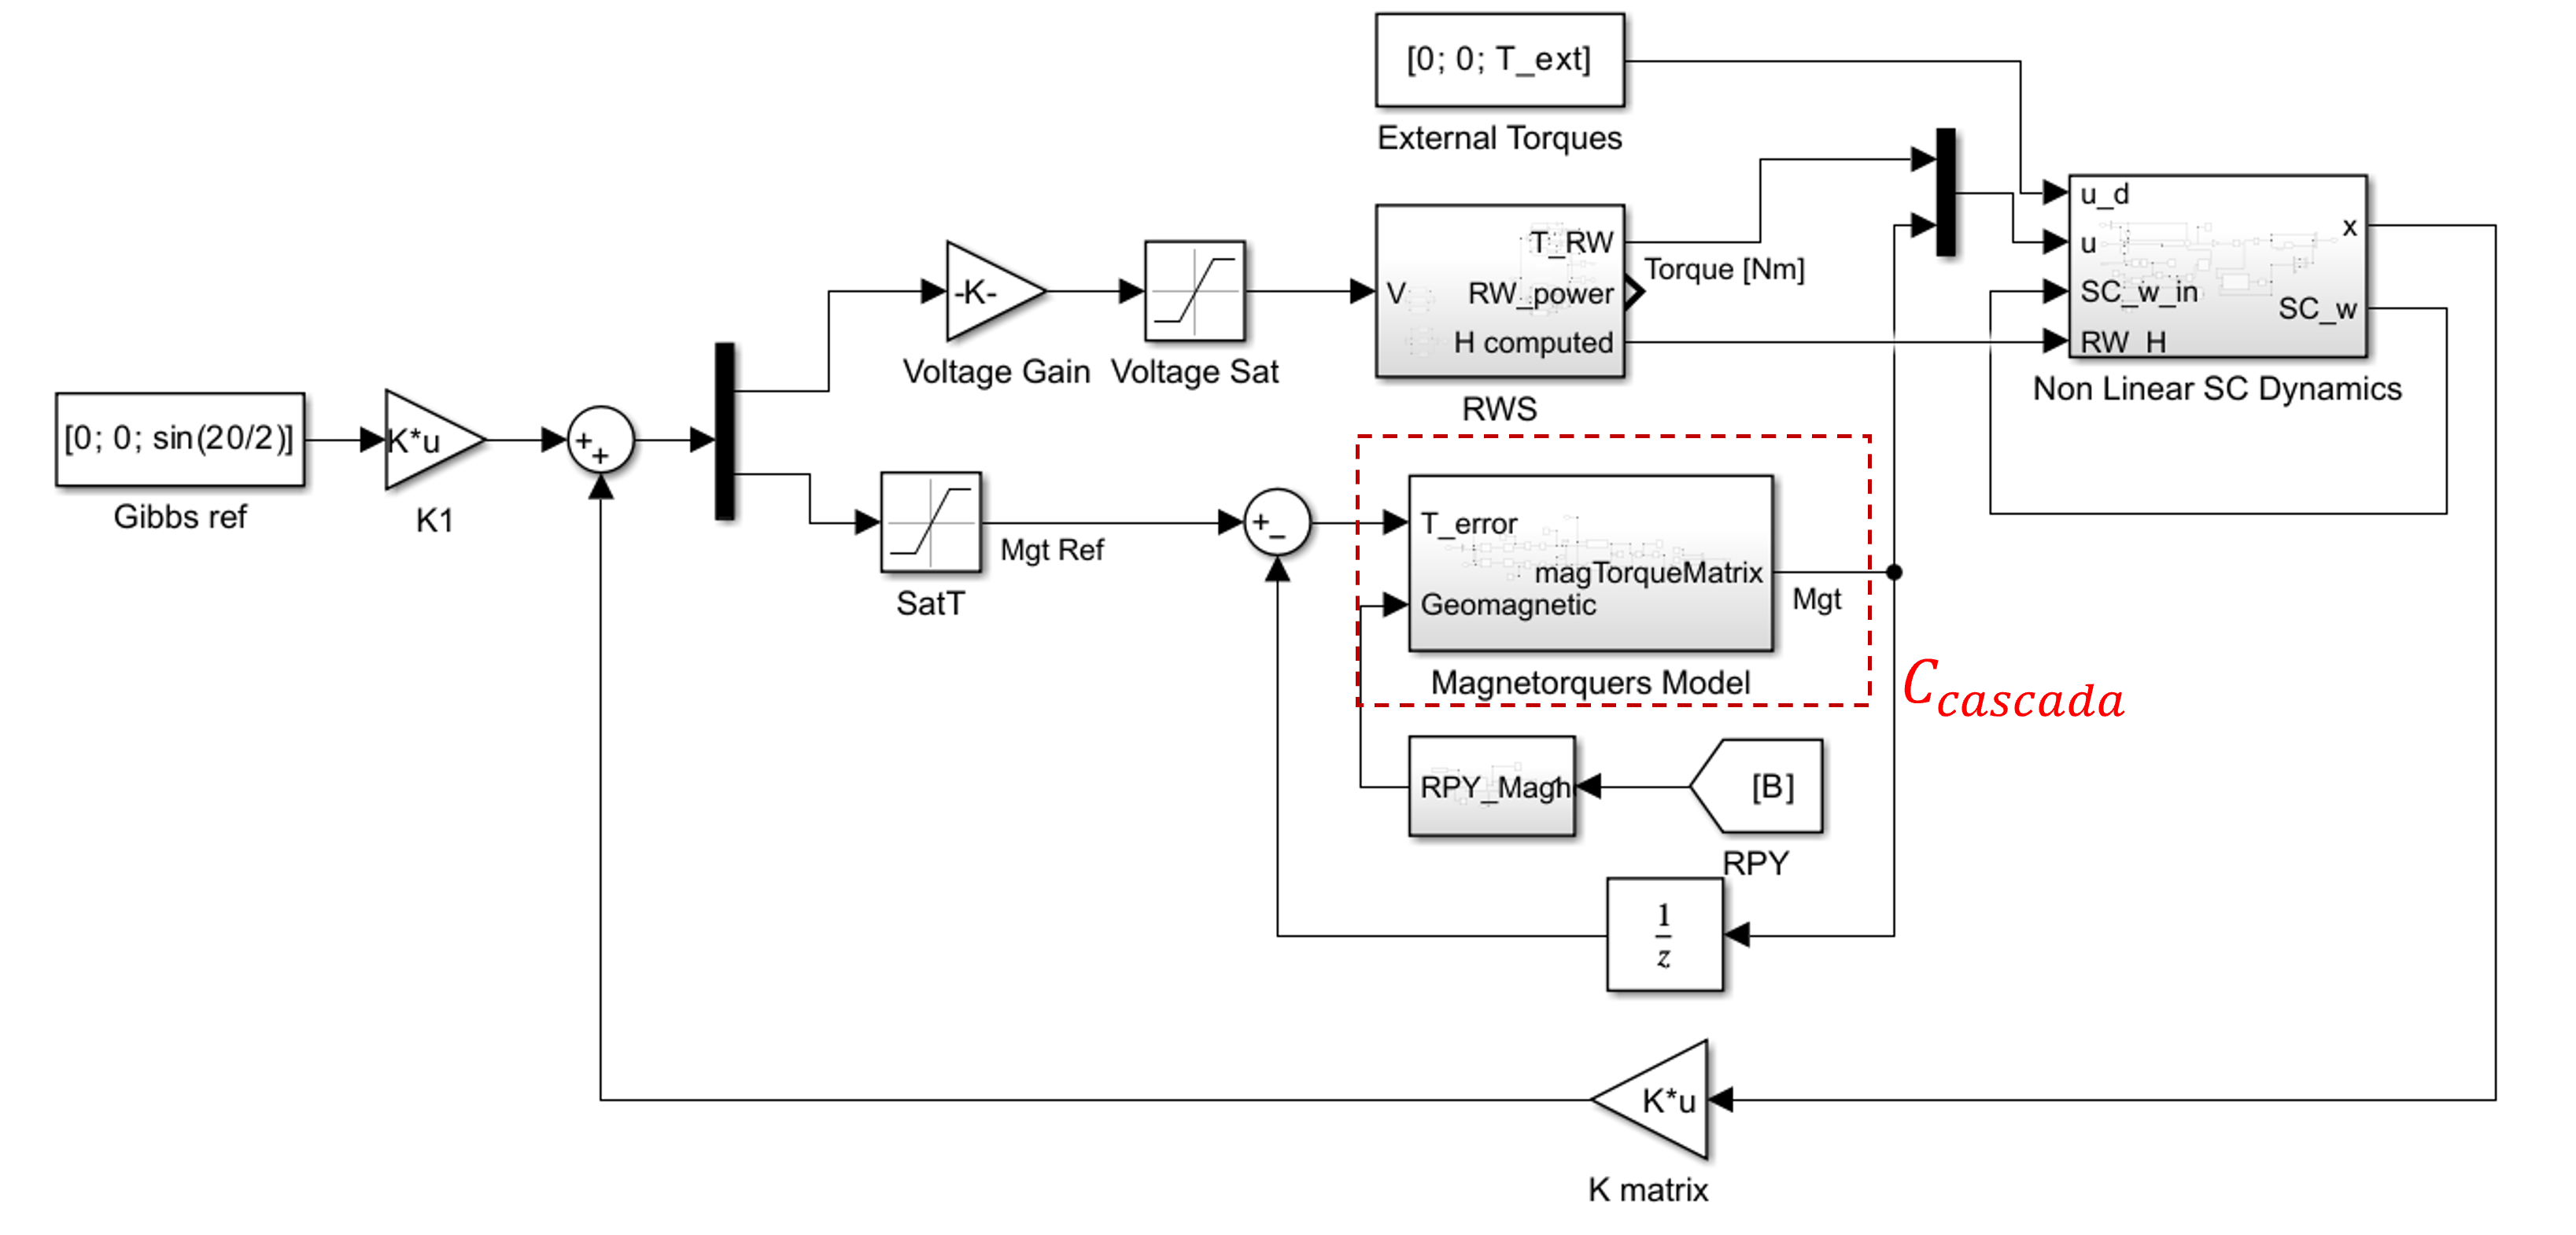
\includegraphics[scale=0.6]{imagenes/controladores/lqr.PNG}\\
	\end{center}
	\caption{LQR simplificado y controlador en cascada con valor de referencia $T_error$.}
	\label{fig:lqr}	 	
\end{figure}

 Finalmente, en la implementación del lazo de control también puede apreciarse el controlador en cascada, el cual recibe su valor de referencia ($T_{error}$) como las componentes correspondientes al torque de los Magnetorquers como se mostró en \textbf{(\ref{eq:estados_y_entradas})} y en \textbf{(\ref{eq:expresionEntradas})}. Internamente, este bloque contiene el modelo de magnetorquers junto con un controlador PID como se evidencia en la \textbf{Fig. (\ref{fig:lqr_cascada})}.
 
\begin{figure}[!ht]
	\begin{center}
		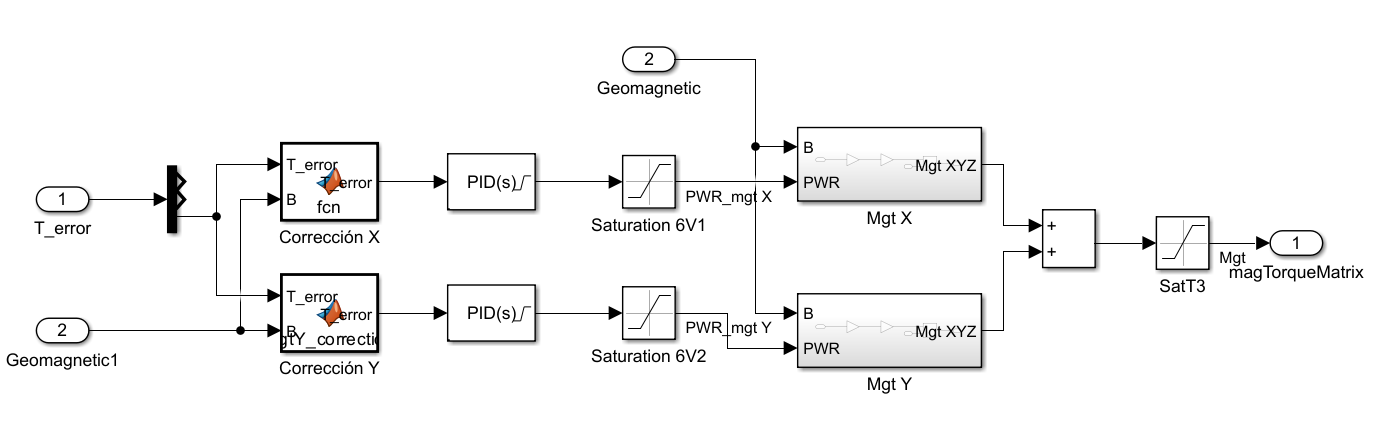
\includegraphics[scale=0.45]{imagenes/controladores/cascada.PNG}\\
	\end{center}
	\caption{Controlador PID en cascada.}
	\label{fig:lqr_cascada}	 	
\end{figure}
\newpage

\subsubsection{PID}
\hfill \break
Usando las herramientas \textit{Control System Designer} y \textit{PID Tuner} de Simulink, fue posible sintonizar los diferentes controladores PID, tanto para el control de actitud como para la desaturación, como se evidencia en las \textbf{Fig. (\ref{fig:PID_Tuning})} y \textbf{Fig. (\ref{fig:PID_Tuning})} respectivamente. 

\begin{figure}[h]
	\centering
	\subfloat[Editor de Root Locus.]{
		\label{fig:PID_Tuning1}
		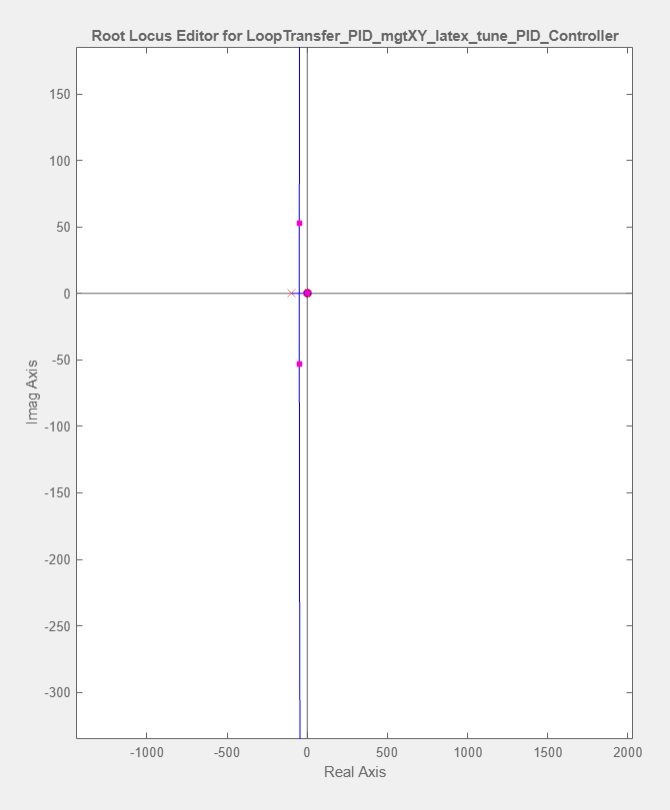
\includegraphics[width=0.37\textwidth]{imagenes/controladores/PID_tuning1_1.PNG}}
	\subfloat[Respuesta al escalón para el control de actitud.]{
		\label{fig:PID_Tuning2}
		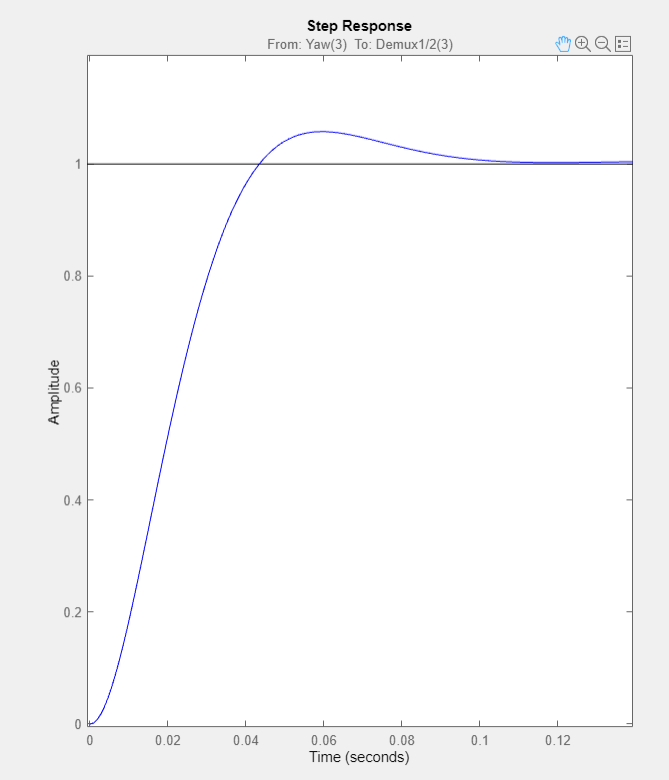
\includegraphics[width=0.382\textwidth]{imagenes/controladores/PID_tuning1_2.PNG}}
	
	\caption{Sintonización PID en Control System Designer.}
	\label{fig:PID_Tuning}
\end{figure}


\begin{figure}[!h]
	\begin{center}
		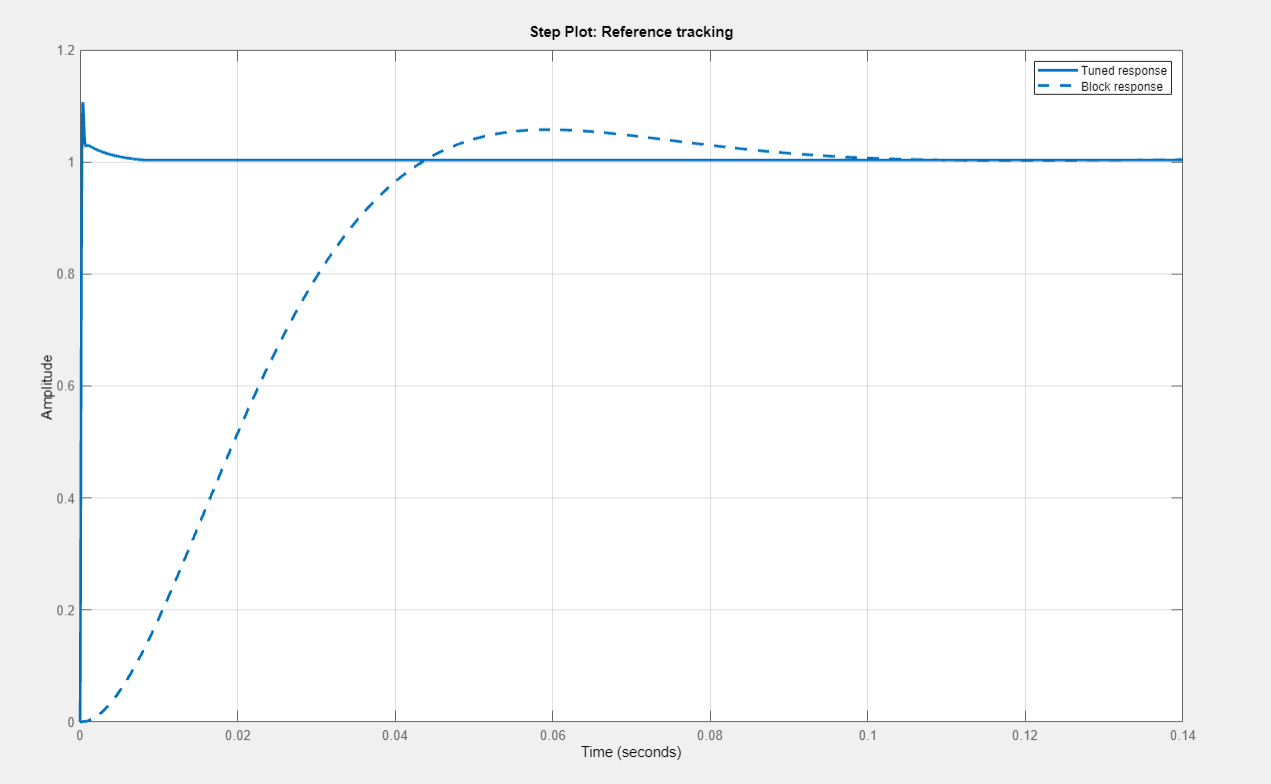
\includegraphics[scale=0.32]{imagenes/controladores/PID_tuning2.PNG}\\
	\end{center}
	\caption{Herramienta PID Tuner para la sintonización controlador PID.}
	\label{fig:PID_tuner}	 	
\end{figure}

% Implementacion 
Ademas de verificar la ubicación de los polos, un ajuste progresivo del controlador fue realizado al evaluar individualmente sus componentes derivativa, integral y proporcional, hasta dar con unas ganancias que permitieran la estabilidad con un bajo tiempo de asentamiento y poca sobreelongación máxima. 

Finalmente, la implementación en Simulink para el control de actitud puede apreciarse en la \textbf{Fig. (\ref{fig:PID})}. De igual forma el modelo de desaturación que cumple la ley de control expresada en la \textbf{ec. (\ref{eq:ley_de_control_sat})} se evidencia en la \textbf{Fig. (\ref{fig:PID_deltaH})}.

\begin{figure}[!ht]
	\begin{center}
		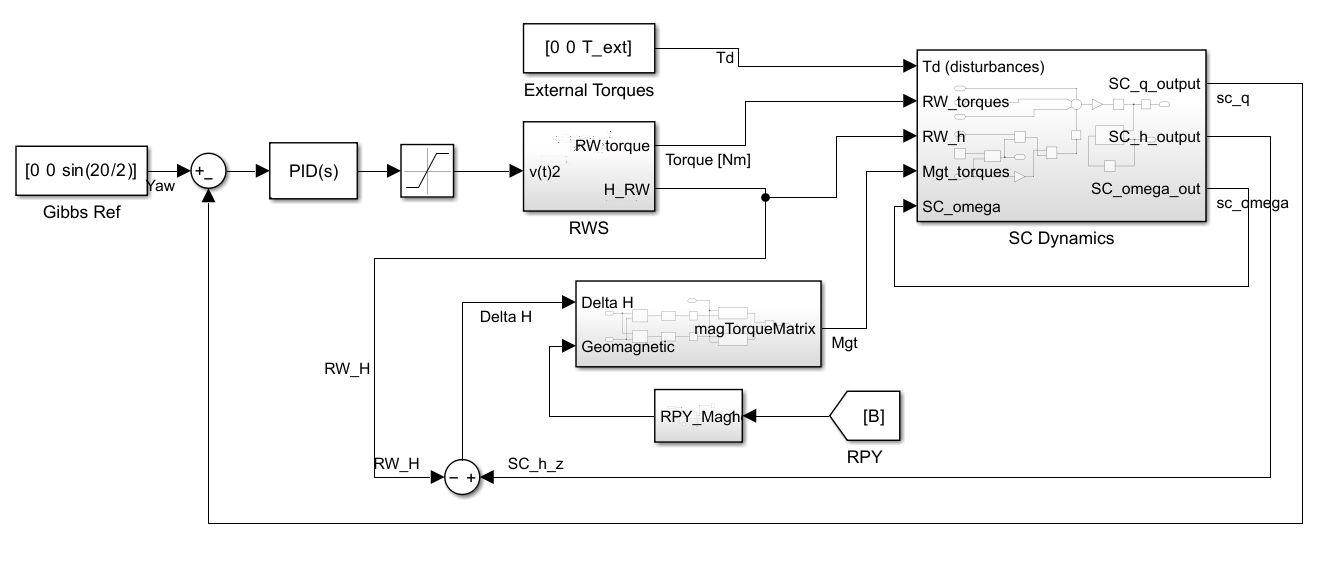
\includegraphics[scale=0.37]{imagenes/controladores/PID.PNG}\\
	\end{center}
	\caption{Implementación simplificada en Simulink del controlador de actitud y desaturación.}
	\label{fig:PID}	 	
\end{figure}

\begin{figure}[!ht]
	\begin{center}
		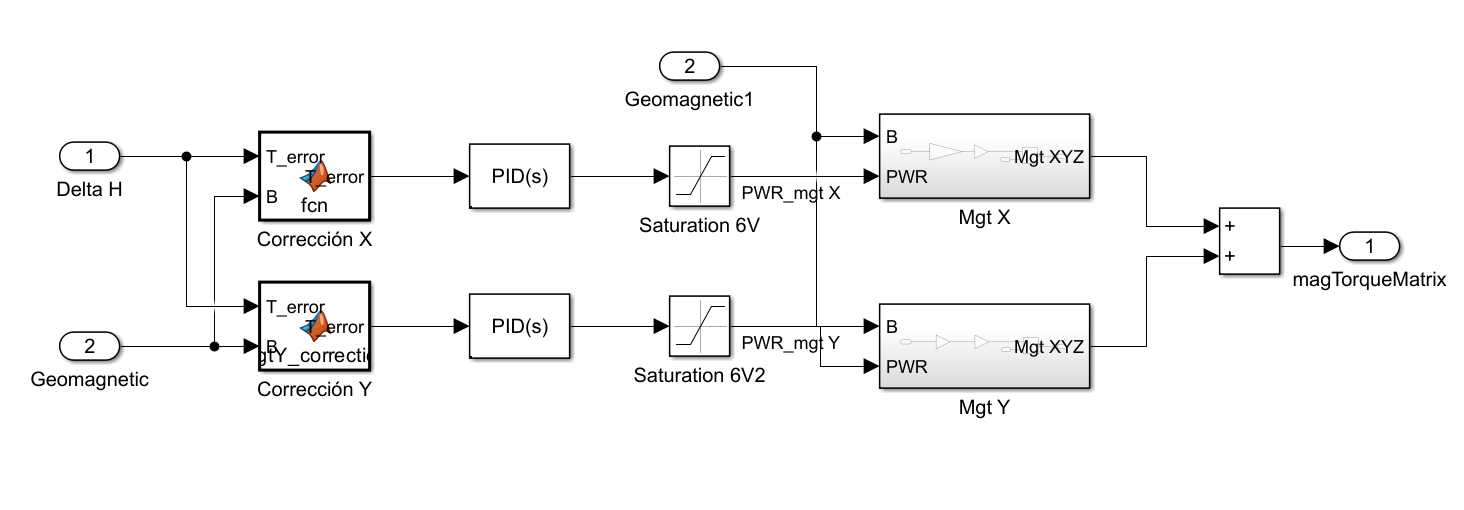
\includegraphics[scale=0.45]{imagenes/controladores/PID_deltaH.PNG}\\
	\end{center}
	\caption{Modelo de desaturación según ley de control de $\Delta h$.}
	\label{fig:PID_deltaH}	 	
\end{figure} 	

\newpage
\subsubsection{Índices de desempeño}
\hfill \break
Con el fin de comparar los diferentes controladores y sus métodos de desaturación, se establecieron indices de desempeño que involucren parámetros clave como el error de referencia, la potencia de los actuadores y la diferencia entre el momento angular del satélite y las RW. Lo anterior se expresa en la siguiente ecuación:
\begin{equation}
	Index = \int_{0}^{\infty} K_{error}\lvert e_{ref}(t)\rvert + K_{\Delta h}\lvert \Delta h(t)\rvert +  K_{RW}\lvert P_{RW}(t)\rvert + K_{mgt}\lvert P_{mgt}(t)\rvert\;dt
\end{equation}

Donde $K_{error}$, $K_{\Delta h}$, $K_{RW}$ y $K_{mgt}$ son las ganancias que permiten mantener cada término del índice de desempeño, en un orden de magnitud cercano para poder ser comparados. Sus valores se recopilaron en la \textbf{Tabla \ref{table:ganancias_indices}}.

\begin{table}[h]
	\caption{\MakeUppercase{Ganancias indices de desempeño }}
	\begin{center}
		\begin{tabular}{ c c c}			
			&  \textbf{Ganancias} &  \textbf{Valor}\\ \hline
			$K_{error}$  &  Error de referencia & $71$ \\ 
			$K_{\Delta h}$ &  Error $\Delta h$ & $132000$ \\ 
			$K_{mgt}$ &  Potencia Magnetorquers & $0.1$ \\ 
			$K_{RW}$ &  Potencia RW & $5$ \\ \hline			
		\end{tabular}
	\end{center}
	\label{table:ganancias_indices}
\end{table}



La implementación para su cálculo en Simulink, tras cada simulación, se evidencia en la \textbf{Fig. (\ref{fig:indicesP})}

\begin{figure}[!h]
	\begin{center}
		\includegraphics[scale=0.35]{imagenes/controladores/indices de desempeño.PNG}\\
	\end{center}
	\caption{Implementación del cálculo de indices de desempeño.}
	\label{fig:indicesP}	 	
\end{figure}

\newpage
\subsubsection{Resumen controladores}
\hfill \break
Debido a que el controlador PID se implementó tanto para el control de actitud como para el método de desaturación, se obtuvieron 3 controladores cuyas ganancias están recopiladas en la \textbf{Tabla \ref{table:gananciasPID}}.

\begin{table}[h]
	\caption{\MakeUppercase{Ganancias controladores PID }}
	\begin{center}
		\begin{tabular}{ c | c c c}
			\textbf{Ganancia}&  \mbox{\boldmath$PID_1$} & \mbox{\boldmath$PID_2$} & \mbox{\boldmath$PID_3$}\\ \hline			
			\textbf{P} &  $4500$ & $0$ & 3739538.59 \\ 
			\textbf{I}  &  $800$ & $2538362.26$ &11683234637.87 \\ 
			\textbf{D}  &  $8000$ & $0$ & -2886.42 \\
			\textbf{N}  &  $100$ & $100$ & 1295.56\\ \hline
			\textbf{Función} &  Control de actitud & Desaturación & Desaturación \\ 			
		\end{tabular}
	\end{center}
	\label{table:gananciasPID}
\end{table}

Finalmente, se obtienen 4 diferentes estrategias de control al combinar los métodos para el control de actitud y la desaturación. En la \textbf{Tabla \ref{table:summary_controllers}} se recopilaron las mejores combinaciones que serán evaluadas en los diferencias escenarios y órbitas.

\begin{table}[h]
	\caption{\MakeUppercase{Recopilación Controladores}}
	\begin{center}
		\begin{tabular}{ c c c c}
			
			ID&  \textbf{Control de actitud} &  \textbf{ Método de desaturación} & \textbf{Controlador desaturación}\\ \hline
			1 &  $PID_1$ & $k\Delta h$ & $PID_2$\\ 
			2 &  $LQR$ & $k\Delta h$ & $PID_2$\\ 
			3 &  $LQR$ & Cascada & $PID_2$\\ 
			4 &  $LQR$ & Cascada  & $PID_3$\\  \hline			
		\end{tabular}
	\end{center}
	\label{table:summary_controllers}
\end{table}
\newpage
%--------------------------

\section{RESULTADOS}
% Mostrar efecto de saturación 
\subsection{Fenómeno de Saturación}

En primer lugar, el fenómeno de saturación fue evidenciado con el fin de visualizar cualitativa-mente el efecto de los magnetorquers en la desaturación. En la \textbf{Fig. \ref{fig:saturacion}} se muestra la respuesta del sistema de ADCS ante un escalón de $-20$ grados en $t=2000\,s$. Debido a que el satélite experimenta torques de perturbaciones $T_{ext} >0$ el torque que deben realizar las RW es negativo, por otro lado, como se sabe que $\tau = \dot{h}$, el momento angular empieza a aumentar con una pendiente negativa conforme pasa el tiempo. Finalmente, es evidente que a medida que las RW se acercan a su nivel de saturación el error del \textit{Yaw} empieza a aumentar como se muestra en la gráfica superior.

\begin{figure}[!h]
	\begin{center}
		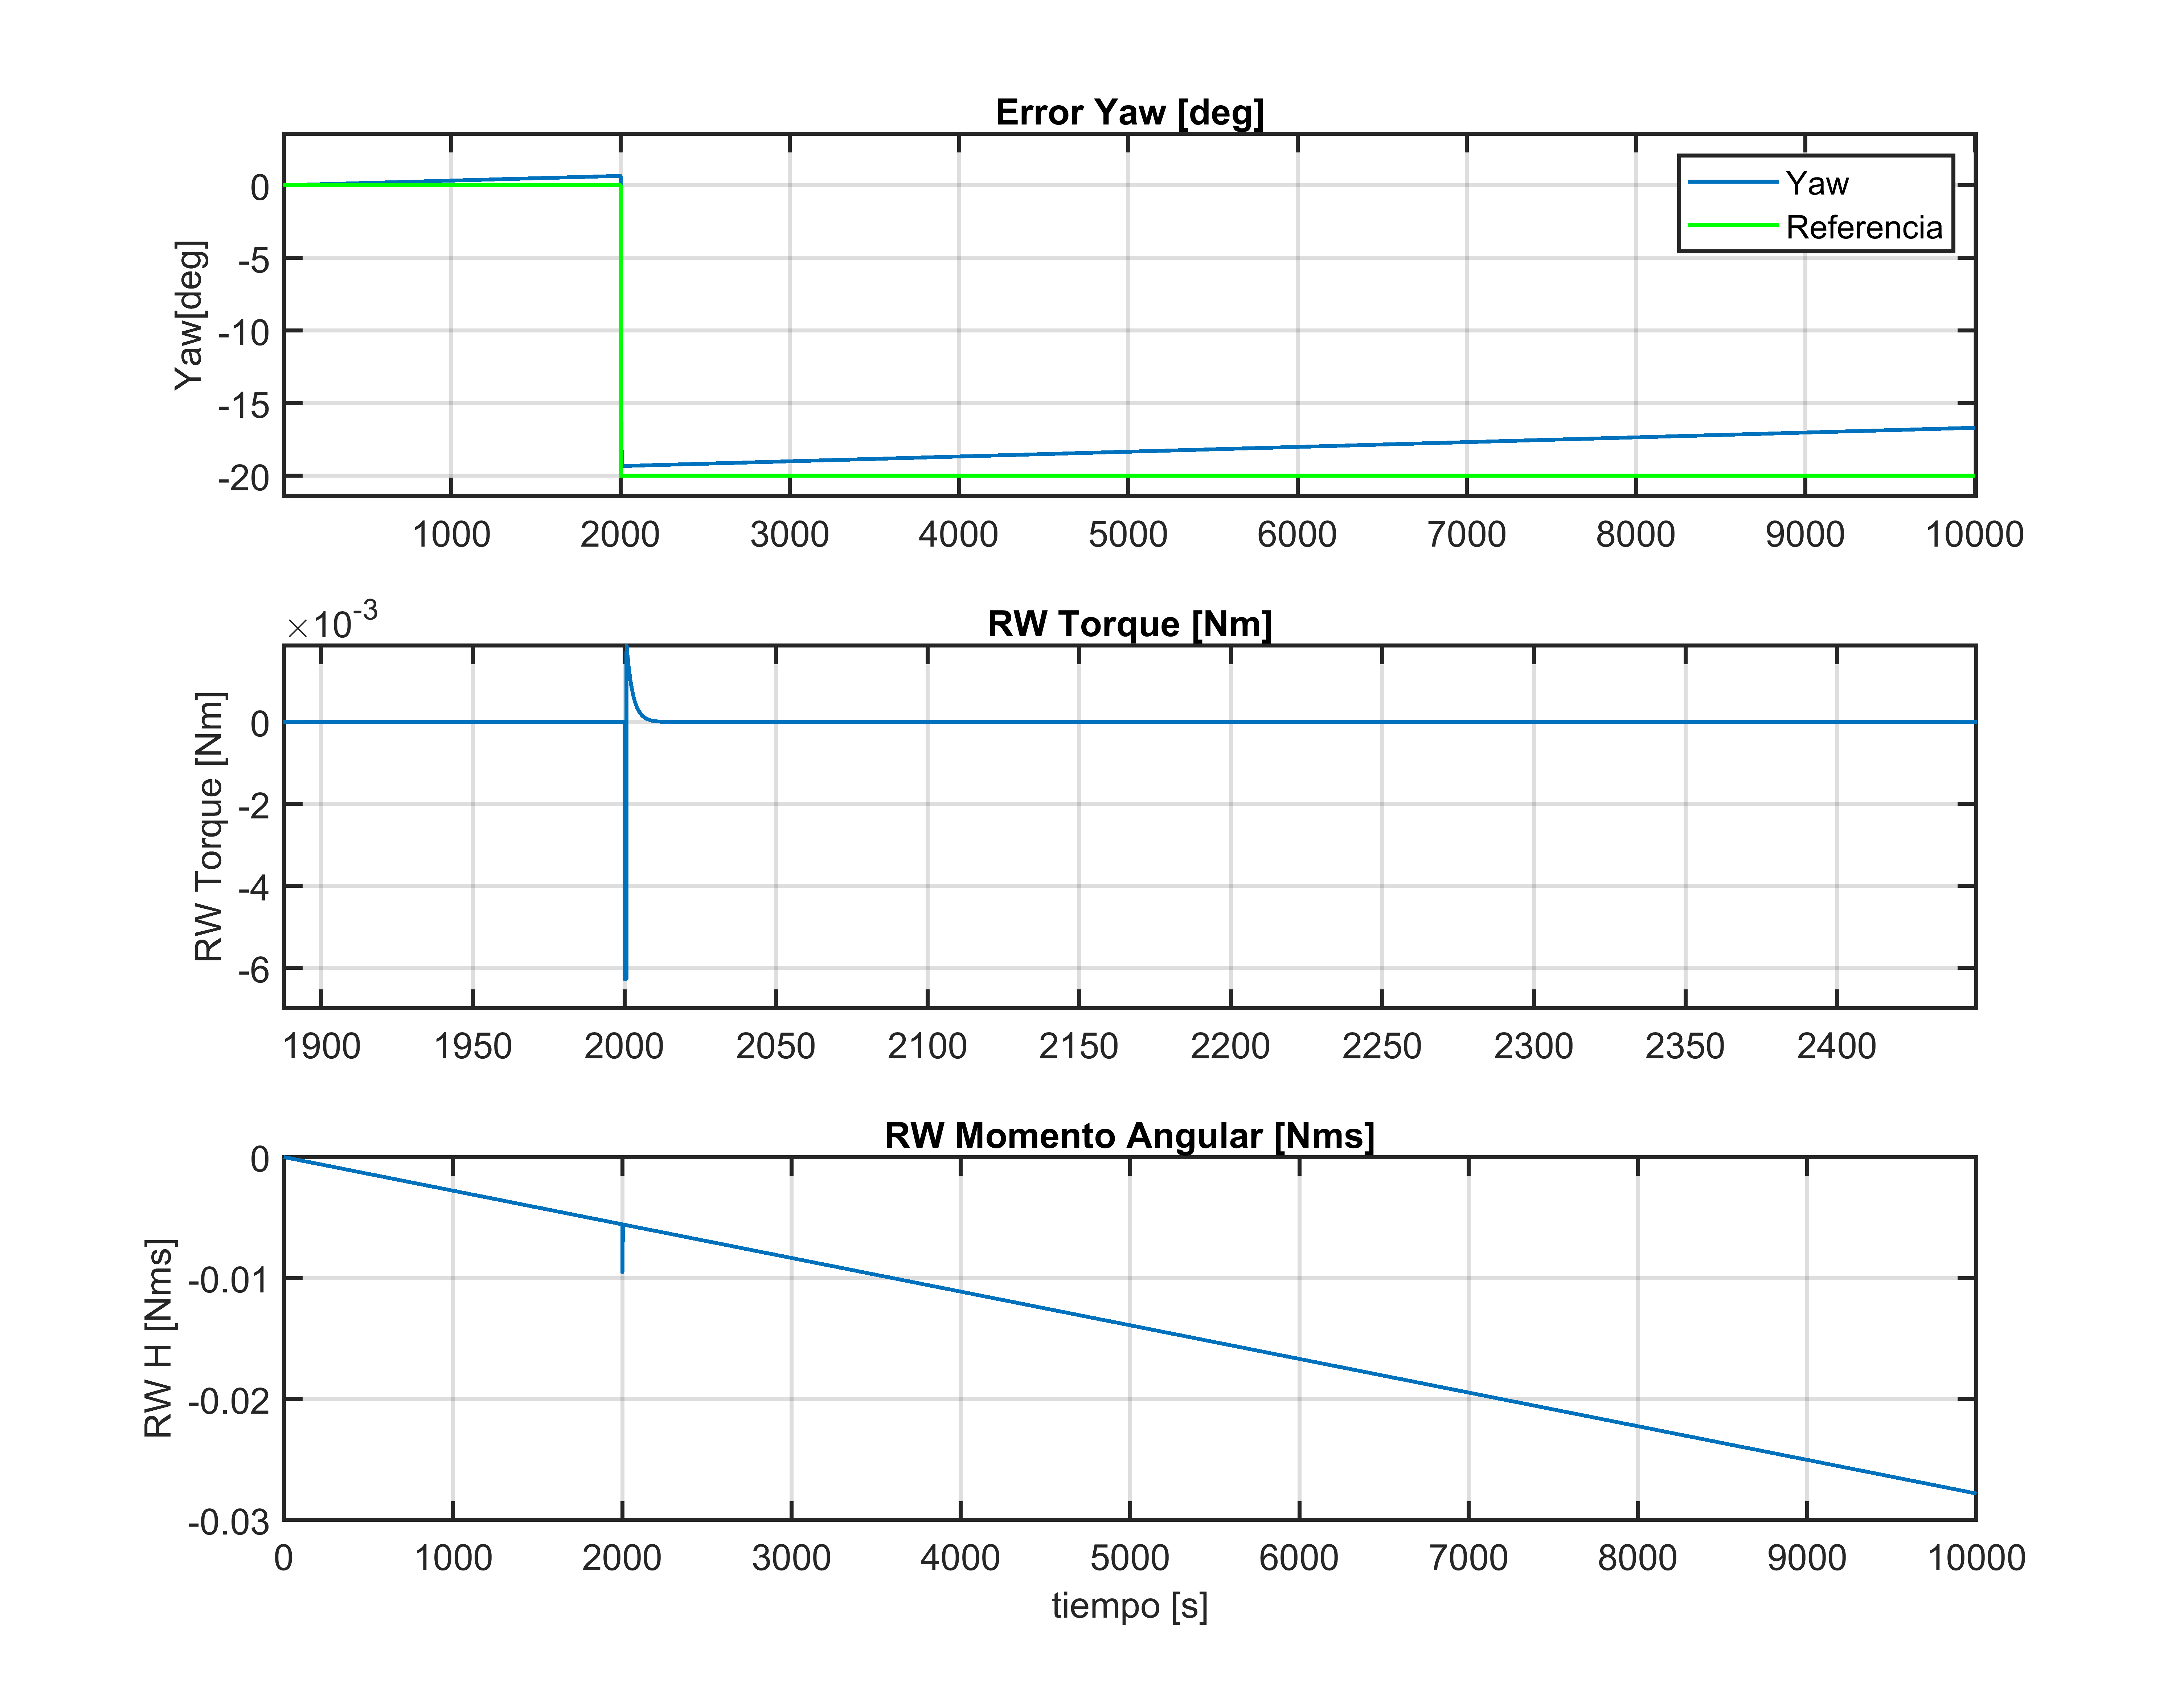
\includegraphics[scale=0.55]{imagenes/resultados/Desaturation.PNG}\\
	\end{center}
	\caption{Saturación en ruedas de reacción y su efecto en el Yaw y momento angular.}
	\label{fig:saturacion}	 	
\end{figure}

\begin{figure}[!ht]
	\begin{center}
		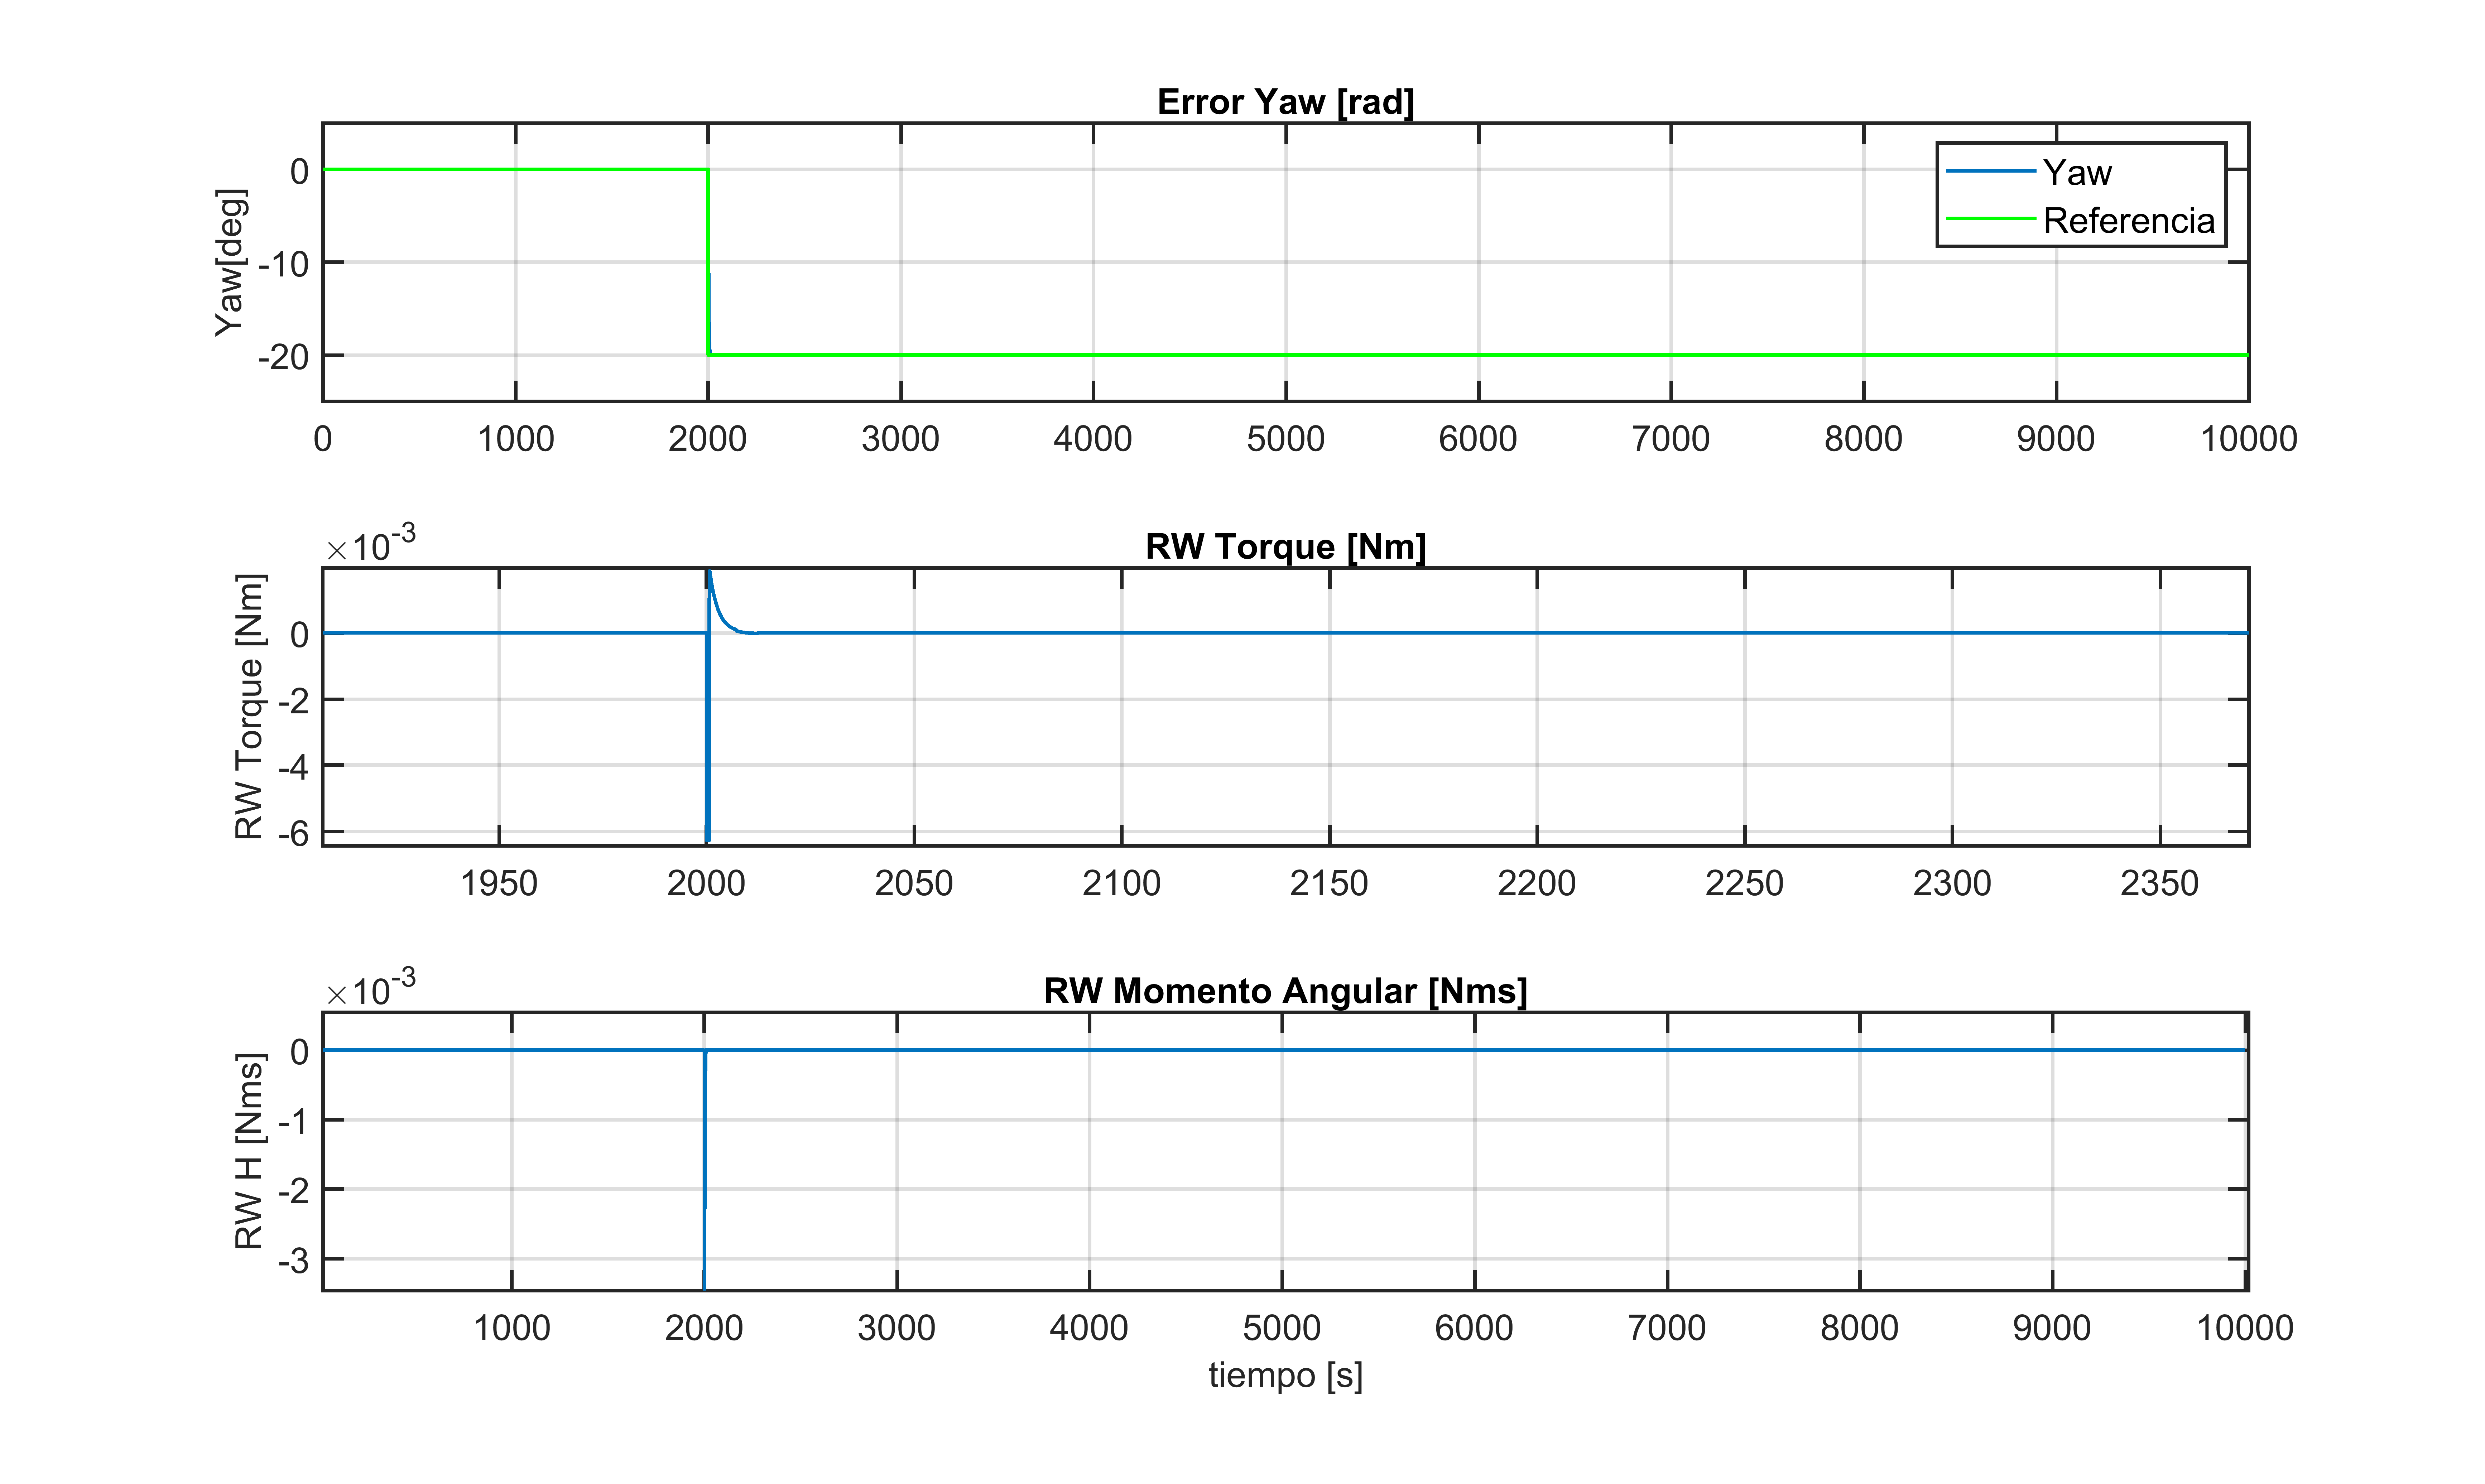
\includegraphics[scale=0.55]{imagenes/resultados/Desaturation2.PNG}\\
	\end{center}
	\caption{Desaturación de RW empleando magnetorquers.}
	\label{fig:desaturacion}	 	
\end{figure}

Una vez se tiene en cuenta el efecto de los magnetorquers y su correspondiente método de saturación, el ADCS puede mantener el ángulo de \textit{Yaw} sin incrementar el error y las ruedas de reacción vuelven a apagarse una vez se realiza la maniobra para alcanzar la actitud deseada. Este caso de desaturación se muestra en la \textbf{Fig. \ref{fig:desaturacion}}.



\newpage
\subsection{Definición de perfiles de misión}
%Descripción de los escenarios a evaluar:
Con el fin de dar solución al planteamiento del problema, se evalúa el desempeño de los controladores en los diferentes escenarios planteados:
\begin{itemize}
	\item \textbf{Fase de \textit{Detumbling}}: Se refiere a la etapa inicial donde se tiene en cuenta una velocidad angular inicial. Esto de debe a las condiciones iniciales que comúnmente enfrentan los satélites al ser desplegados en LEO. Recurriendo a \cite{Ofodile2019}, se tomó un valor de referencia de $\omega_{o} = 0.29\,rad/s$.
	 
	\item \textbf{Respuesta tipo escalón}: Se establece una referencia para un ángulo de \textit{Yaw} deseado. Para las simulaciones se tomó un valor de $20$ grados donde este se duplica al cabo de unos segundos para tener un doble escalón.
	\newpage 
	\item \textbf{Apuntamiento hacia el Nadir}: Con el fin de simular un apuntamiento constante a la tierra se evalúa una respuesta tipo rampa para alcanzar una velocidad de rotación constante que corresponda con la velocidad angular de la órbita. Para ello se determinó el periodo orbital $T_o$ y la velocidad angular con las expresiones:
	\begin{gather}
		T_o = 2\pi\sqrt{\frac{a^3}{GM}}\\
		\omega = \frac{2\pi}{T_o} = 0.0635\,deg/s 
	\end{gather}
	
	Donde $a$, $G$ y $M$ son el semi eje mayor, la constante de gravitación y la masa de la tierra respectivamente.
\end{itemize} 

\begin{figure}[!h]
	\begin{center}
		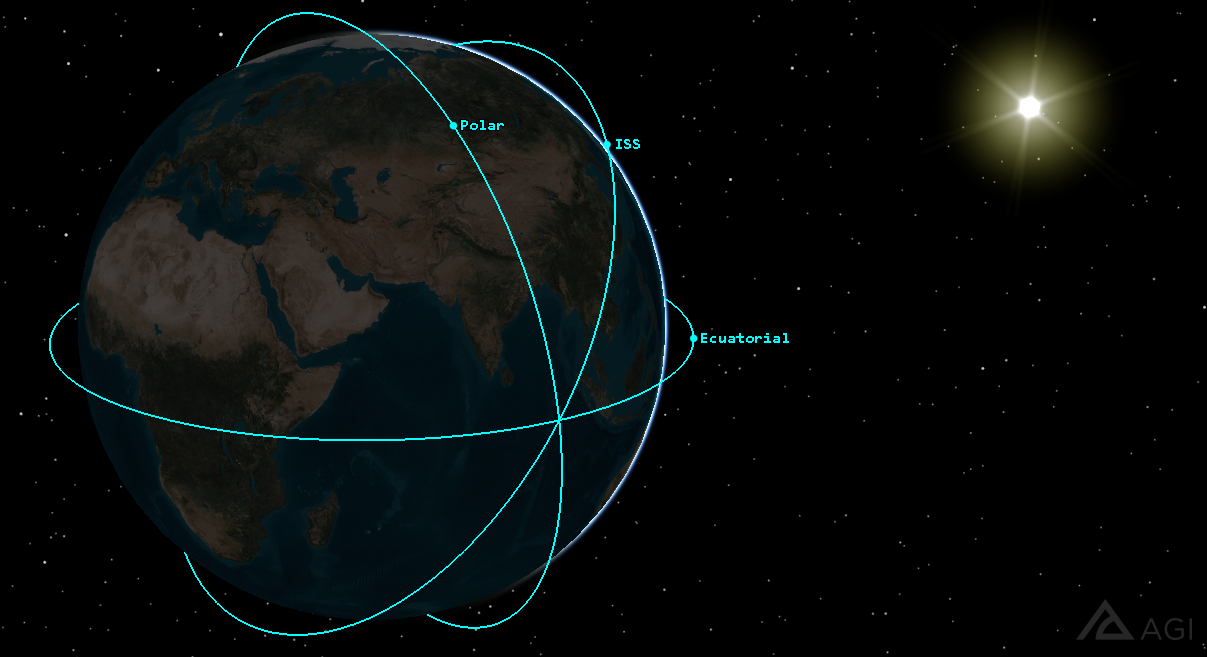
\includegraphics[scale=0.40]{imagenes/resultados/orbitas.PNG}\\
	\end{center}
	\caption{Órbitas evaluadas en los diferentes perfiles de misión representadas en STK\textsuperscript{\tiny\textregistered}}
	\label{fig:orbitas_eval}	 	
\end{figure}

Por otro lado, los perfiles de misión mencionados anteriormente se evalúan en 3 órbitas diferentes con el fin de comparar el rendimiento de los magnetorquers según el campo magnético que atraviese el satélite. La representación de las órbitas puede apreciarse en la \textbf{Fig. \ref{fig:orbitas_eval}} y sus elementos orbitales se consignaron en la \textbf{Tabla \ref{table:Parametros_orbitales}}.


% Imagen y parámetros orbitales 
%Sujeto a 3 tipos de órbita 



\begin{table}[!ht]
	\caption{\MakeUppercase{Parámetros Orbitales de las trayectorias a evaluar }}
	\begin{center}
		\begin{tabular}{ c c c c c}
			
			&  \textbf{Elemento orbital} &  \textbf{Ecuatorial} & \textbf{ISS }& \textbf{Polar}\\ \hline
			\noindent$RAAN$& Ascensión recta del nodo ascendente [deg] &75.84 & 75.84 & 75.84 \\
			$\omega$& Argumento de perigeo [deg] & 180& 180 & 180 \\
			$\nu$&Anomalía verdadera[deg] &16.3 & 16.3 &16.3\\
			$i$&Inclinación[deg] & 0 & 57 &98\\
			$a$&Semi eje mayor [km] & 6978  & 6978&6978\\
			$e$&Excentricidad &0.0004681 &0.0004681 & 0.0004681 \\ \hline			
		\end{tabular}
	\end{center}
	\label{table:Parametros_orbitales}
\end{table}

A continuación se mostrarán los resultados de ángulo de \textit{Yaw}, velocidad angular del satélite y momento angular de las RW para los 3 perfiles de misión en sus respectivas órbitas. Adicionalmente, se recopilaron los indices de desempeño de los controladores que son de utilidad para su comparación. 
\newpage
\subsection{Perfil de misión 1: Detumbling}
% Tabla indices de desempeño ecuatorial Detumbling
 
\begin{table}[!h]
	\label{table:Detumbling_ecuatorial}
	\caption{\MakeUppercase{Indices de desempeño para órbita ecuatorial en maniobra de Detumbling}}
	\centering
	\begin{tabular}{r|lllll|l}
		\multicolumn{1}{l|}{\textbf{ID}} & \textbf{Controlador}                  & \mbox{\boldmath$e_{ref}$}   & \mbox{\boldmath$\Delta h$} & \mbox{\boldmath$P_{RW}$}   & \mbox{\boldmath$P_{mgt}$}    & \textbf{Total}      \\ 
		\hline
		1                       & PID $\Delta h$ & 29.39  & 931.32     & 88.79  & 339.68 & 1389.19  \\
		2                       & LQR $\Delta h$ & 291.75 & 926.60   & 332.94 & 340.04 & 1891.34  \\
		3                       & LQR I          & 283.27 & 935.20     & 332.26 & 343.67 & 1894.41  \\
		4                       & LQR PID        & 275.73& 933.24      & 320.65 & 340.40 & 1870.03  \\
		\hline
%		\cline{1-2}\cline{4-7}
	\end{tabular}
\end{table}


% Tabla indices de desempeño ISS Detumbling
\begin{table}[!h]
	\label{table:Detumbling_iss}
	\caption{\MakeUppercase{Indices de desempeño para órbita de la ISS en maniobra de Detumbling }}
	\centering
	\begin{tabular}{r|lllll|l}
		\multicolumn{1}{l|}{\textbf{ID}} & \textbf{Controlador}                  & \mbox{\boldmath$e_{ref}$}   & \mbox{\boldmath$\Delta h$} & \mbox{\boldmath$P_{RW}$}   & \mbox{\boldmath$P_{mgt}$}    & \textbf{Total}      \\ 
		\hline
		1                       & PID $\Delta h$ & 29.33  & 709.51     & 88.83  & 346.15 & 1173.83  \\
		2                       & LQR $\Delta h$ & 225.91 & 708.36     & 332.34 & 346.89 & 1613.49  \\
		3                       & LQR I          & 227.33 & 714.92     & 331.37 & 345.31 & 1618.94  \\
		4                       & LQR PID        & 234.43 & 711.95     & 319.50 & 348.44 & 1614.33  \\
		\hline
		%		\cline{1-2}\cline{4-7}
	\end{tabular}
\end{table}

% Tabla indices de desempeño Polar Detumbling 

\begin{table}[!h]
	\label{table:Detumbling_polar}
	\caption{\MakeUppercase{Indices de desempeño para órbita polar en maniobra de Detumbling}}
	\centering
	\begin{tabular}{r|lllll|l}
		\multicolumn{1}{l|}{\textbf{ID}} & \textbf{Controlador}                  & \mbox{\boldmath$e_{ref}$}   & \mbox{\boldmath$\Delta h$} & \mbox{\boldmath$P_{RW}$}   & \mbox{\boldmath$P_{mgt}$}    & \textbf{Total}      \\ 
		\hline
		1                       & PID $\Delta h$ & 29.38 & 929.53& 88.88 & 414.89 & 1462.68  \\
		2                       & LQR $\Delta h$ & 277.68 & 928.36 &332.43 &409.66 & 1948.14  \\
		3                       & LQR I          & 282.22 & 932.90 &330.22 & 415.75 &1961.08  \\
		4                       & LQR PID        & 326.09 & 932.21 & 327.58 & 399.09 & 1984.97  \\
		\hline
		%		\cline{1-2}\cline{4-7}
	\end{tabular}
\end{table}
\clearpage

% Graficas de las 3 orbitas Detumbling

\begin{figure}[!ht]
	\centering
	\begin{subfigure}{1.2\linewidth}
		
\includegraphics[width=\linewidth]{imagenes/resultados/Detumbling/orbit_zero/yaw_omega_h_zero.PNG}
		\caption{Órbita ecuatorial}
		\label{fig:orbita_ecuatorial_Detumbling}
	\end{subfigure}\\
	\begin{subfigure}{1.2\linewidth}
		\includegraphics[width=\linewidth]{imagenes/resultados/Detumbling/orbit_iss/yaw_omega_h_iss.PNG}
		\caption{Órbita ISS}
		\label{fig:orbita_iss_Detumbling}
	\end{subfigure}\\
	\begin{subfigure}{1.2\linewidth}
		\includegraphics[width=\linewidth]{imagenes/resultados/Detumbling/orbit_polar/yaw_omega_h_polar.PNG}
		\caption{Órbita polar}
		\label{fig:orbita_polar_Detumbling}
	\end{subfigure}
	\caption{Ángulo de Yaw, velocidad angular del S/C y momento angular de las RW para el perfil de misión de Detumbling}
	\label{fig:Detumbling_ecuatorial}
\end{figure}
\clearpage
\subsection{Perfil de misión 2: Escalón}

\begin{table}[!h]\label{table:step_ecuatorial}	
	\caption{\MakeUppercase{Indices de desempeño para órbita ecuatorial en respuesta del escalón}}
	\centering
	\begin{tabular}{r|lllll|l}
		\multicolumn{1}{l|}{\textbf{ID}} & \textbf{Controlador}                  & \mbox{\boldmath$e_{ref}$}   & \mbox{\boldmath$\Delta h$} & \mbox{\boldmath$P_{RW}$}   & \mbox{\boldmath$P_{Mgt}$}    & \textbf{Total}      \\ 
		\hline
		1                       & PID $\Delta h$ & 155.78 & 0.0046 &83.26 &1.85 &240.91  \\
		2                       & LQR $\Delta h$ & 120.31 & 0.0043     &64.12   &1.83    & 186.27  \\
		3                       & LQR I          & 120.23 & 0.24      &64.19   &8.32    & 192.98  \\
		4                       & LQR PID        & 119.71 & 0.25      &63.66 & 8.54 & 192.17  \\
		\hline
		%		\cline{1-2}\cline{4-7}
	\end{tabular}
\end{table}


% Tabla indices de desempeño ISS Step
\begin{table}[!h]\label{table:step_iss}	
	\caption{\MakeUppercase{Indices de desempeño para órbita de la ISS en respuesta del escalón }}
	\centering
	\begin{tabular}{r|lllll|l}
		\multicolumn{1}{l|}{\textbf{ID}} & \textbf{Controlador}                  & \mbox{\boldmath$e_{ref}$}   & \mbox{\boldmath$\Delta h$} & \mbox{\boldmath$P_{RW}$}   & \mbox{\boldmath$P_{Mgt}$}    & \textbf{Total}      \\ 
		\hline
		1                       & PID $\Delta h$ & 155.97 & 0.0061& 83.34 & 2.76& 242.08  \\
		2                       & LQR $\Delta h$ & 120.55 & 0.0046 &64.25 &2.41 & 187.21  \\
		3                       & LQR I          & 120.07 & 0.24       &64.12  & 7.97 &192.41  \\
		4                       & LQR PID        & 119.85 & 0.24       & 63.85 &9.15 &  193.09  \\
		\hline
		%		\cline{1-2}\cline{4-7}
	\end{tabular}
\end{table}

% Tabla indices de desempeño Polar Step 

\begin{table}[!h]\label{table:step_polar}
	\caption{\MakeUppercase{Indices de desempeño para órbita polar en respuesta del escalón}}
	\centering
	\begin{tabular}{r|lllll|l}
		\multicolumn{1}{l|}{\textbf{ID}} & \textbf{Controlador}                  & \mbox{\boldmath$e_{ref}$}   & \mbox{\boldmath$\Delta h$} & \mbox{\boldmath$P_{RW}$}   & \mbox{\boldmath$P_{Mgt}$}    & \textbf{Total}      \\ 
		\hline
		1                       & PID $\Delta h$ & 155.99& 0.0019& 83.06 &6.90 &245.96  \\
		2                       & LQR $\Delta h$ & 120.43 & 0.002 & 64.18 &7.35 &191.97  \\
		3                       & LQR I          & 119.97& 0.235 &64.01 &9.64 &193.87  \\
		4                       & LQR PID        & 120.18 & 0.25 &63.88 &9.89 &194.22  \\
		\hline
		%		\cline{1-2}\cline{4-7}
	\end{tabular}
\end{table}
\clearpage

% Gráficas para Escalón
\begin{figure}
	\centering
	\begin{subfigure}{1.2\linewidth}
		\includegraphics[width=\linewidth]{imagenes/resultados/Step/orbit_zero/Compilado.PNG}
		\caption{Órbita ecuatorial}
		\label{fig:step_zero}
	\end{subfigure}\\
	\begin{subfigure}{1.2\linewidth}
		\includegraphics[width=\linewidth]{imagenes/resultados/Step/orbit_iss/Compilado.PNG}
		\caption{Órbita ISS}
		\label{fig:step_iss}
	\end{subfigure}\\
	\begin{subfigure}{1.2\linewidth}
		\includegraphics[width=\linewidth]{imagenes/resultados/Step/orbit_polar/Compilado.PNG}
		\caption{Órbita Polar}
		\label{fig:step_polar}
	\end{subfigure}
	\caption{Ángulo de Yaw, velocidad angular del S/C y momento angular de las RW para el perfil de misión escalón.}
	\label{fig:step}
\end{figure}
\clearpage
\subsection{Perfil de misión 3 : Apuntamiento hacia el Nadir}

\begin{table}[!h]
	\label{table:nadir_ecuatorial}
	\caption{\MakeUppercase{Indices de desempeño para órbita ecuatorial en apuntamiento Nadir}}
	\centering
	\begin{tabular}{r|lllll|l}
		\multicolumn{1}{l|}{\textbf{ID}} & \textbf{Controlador}                  & \mbox{\boldmath$e_{ref}$}   & \mbox{\boldmath$\Delta h$} & \mbox{\boldmath$P_{RW}$}   & \mbox{\boldmath$P_{Mgt}$}    & \textbf{Total}      \\ 
		\hline
		1                       & PID $\Delta h$ & 0.00094 &0.0039& 0.040& 2.01 &2.06  \\
		2                       & LQR $\Delta h$ & 0.95 & 0.0046& 0.00071& 2.075& 3.03  \\
		3                       & LQR I          & 0.903 &0.180 &0.00063 &2.059 &3.14  \\
		4                       & LQR PID        & 0.903& 0.181 &0.00063 &11.42 &12.51  \\
		\hline
		%		\cline{1-2}\cline{4-7}
	\end{tabular}
\end{table}


% Tabla indices de desempeño ISS Nadir
\begin{table}[!h]
	\label{table:nadir_iss}
	\caption{\MakeUppercase{Indices de desempeño para órbita de la ISS en apuntamiento Nadir}}
	\centering
	\begin{tabular}{r|lllll|l}
		\multicolumn{1}{l|}{\textbf{ID}} & \textbf{Controlador}                  & \mbox{\boldmath$e_{ref}$}   & \mbox{\boldmath$\Delta h$} & \mbox{\boldmath$P_{RW}$}   & \mbox{\boldmath$P_{Mgt}$}    & \textbf{Total}      \\ 
		\hline
		1                       & PID $\Delta h$ &0.00094 &0.0038 &0.040 &2.49& 2.54  \\
		2                       & LQR $\Delta h$ & 0.95 &0.0036751& 0.00069 &2.46 &3.42  \\
		3                       & LQR I          & 0.90 &0.18007 &0.000629 &2.43 &3.51 \\
		4                       & LQR PID        & 0.90 &0.18031 &0.000631& 1.6284 &2.71  \\
		\hline
		%		\cline{1-2}\cline{4-7}
	\end{tabular}
\end{table}

% Tabla indices de desempeño Polar Nadir 

\begin{table}[!h]
	\label{table:nadir_polar}
	\caption{\MakeUppercase{Indices de desempeño para órbita polar en apuntamiento Nadir}}
	\centering
	\begin{tabular}{r|lllll|l}
		\multicolumn{1}{l|}{\textbf{ID}} & \textbf{Controlador}                  & \mbox{\boldmath$e_{ref}$}   & \mbox{\boldmath$\Delta h$} & \mbox{\boldmath$P_{RW}$}   & \mbox{\boldmath$P_{Mgt}$}    & \textbf{Total}      \\ 
		\hline
		1                       & PID $\Delta h$ & 0.00096& 0.0037& 0.040 &3.47 &3.52  \\
		2                       & LQR $\Delta h$ & 0.952 &0.0035& 0.00069 &3.48 &4.44 \\
		3                       & LQR I          & 0.903& 0.18& 0.000643& 4.55& 5.63\\
		4                       & LQR PID        & 0.903 &0.18& 0.000604& 4.35 &5.43 \\
		\hline
		%		\cline{1-2}\cline{4-7}
	\end{tabular}
\end{table}
\clearpage

%Graficas Nadir
\begin{figure}
	\centering
	\begin{subfigure}{1.2\linewidth}
		\includegraphics[width=\linewidth]{imagenes/resultados/Nadir/orbit_zero/Compilado2.PNG}
		\caption{Órbita ecuatorial}
		\label{fig:nadir_zero}
	\end{subfigure}\\
	\begin{subfigure}{1.2\linewidth}
		\includegraphics[width=\linewidth]{imagenes/resultados/Nadir/orbit_iss/Compilado2.PNG}
		\caption{Órbita ISS}
		\label{fig:nadir_iss}
	\end{subfigure}\\
	\begin{subfigure}{1.2\linewidth}
		\includegraphics[width=\linewidth]{imagenes/resultados/Nadir/orbit_polar/Compilado2.PNG}
		\caption{Órbita Polar}
		\label{fig:nadir_polar}
	\end{subfigure}
	\caption{Ángulo de Yaw, velocidad angular del S/C y momento angular de las RW para el perfil de misión apuntamiento Nadir.}
	\label{fig:nadir}
\end{figure}  
\clearpage

%En los resultados se comunican los hallazgos y descubrimientos del estudio. Se incluyen tablas, figuras, diagramas y demás material demostrativo.
%
%
%
%
% Al narrar descriptivamente una figura, tabla, etc., en un párrafo, puedes insertar una referencia cruzada, es decir, un hipervínculo al elemento mencionado dentro o fuera de paréntesis, ejemplos: estos resultados se muestran en la \textbf{Tabla \ref{table:prob_milenio}}.  Igualmente, los datos son validados con otros instrumentos \textbf{(Tabla \ref{table:num_mersenne}, Tabla \ref{table:medalla_fields})}. Lineamientos que se establecen en la nueva versión de las Normas APA séptima edición \textbf{(Fig. \ref{figportada_apa})}. La producción intelectual institucional se publica en el Repositorio \textbf{(Fig. \ref{fig:escudo_udea})}. Si la figura es de tu completa autoría, \textbf{NO} es necesario colocar la leyenda “Elaboración propia” \textbf{(Fig. \ref{fig:hiperbolica})}.

%\begin{figure}[!ht]
%    \begin{center}
%    \includegraphics[scale=0.5]{imagenes/grafica.png}\\
%    \end{center}
%    \caption{Función hiperbólica}
%    \label{fig:hiperbolica}
%    \textit{}
%\end{figure}

%\begin{table}%[!ht]
%\caption{\MakeUppercase{Problemas del milenio: la resolucion de uno de estos problemas se premian con un monto de us\$ 1 millon}}
%\begin{center}
%\begin{tabular}{  l c }
%    \hline
%    1 & El problema de $P$ frente a $NP$  \\ \hline
%    2 &  La conjetura de Hodge \\ \hline
%    3 &  La conjetura de Poincaré \\ \hline
%    4 &  La hipótesis de Riemann \\ \hline
%    5 &  Yang-Mills y el salto de masa ("mass gap")\\ \hline
%    6 &  Las ecuaciones de Navier-Stokes\\ \hline
%    7 &  Conjetura de Birch y Swinnerton-Dyer\\
%        \hline
%\end{tabular}
%\end{center}
%\label{table:prob_milenio}
%\end{table}

%%\clearpage
%
%
%\clearpage
%
%\begin{table}%[!ht]
%\caption{\MakeUppercase{Algunos números primos de Mersenne}}
%\begin{center}
%\begin{tabular}{ c|c}
%    \hline
%    Exponente $n$ & Primo de Mersenne \\ \hline
%    2 &  $2^{2}-1=3 $ \\ \hline
%    3 &  $2^{3}-1=7 $ \\ \hline
%    5 &  $2^{5}-1=31 $ \\ \hline
%    7 &  $2^{7}-1=127 $ \\ \hline
%    13 &  $2^{13}-1=8191 $ \\ \hline
%    17 &  $2^{17}-1=131071 $ \\
%        \hline
%\end{tabular}
%\end{center}
%\label{table:num_mersenne}
%\end{table}
%
%
%\begin{figure}[!ht]
%    \begin{center}
%    \includegraphics[scale=0.5]{imagenes/ieee_logo.jpg}\\
%    \end{center}
%    \caption{Imagen corporativa Institute of Electrical and Electronics Engineers (IEEE)}
%    \label{figportada_apa}
%    \footnotesize{Nota. Fuente \url{https://www.ieee.org/} Esta entidad edita y normaliza la presentación de documentos científicos en el área de ingenierías.} %\citep{lib:apa}.
%\end{figure}
%
%\clearpage
%
%\begin{figure}[!ht]
%    \begin{center}
%    \includegraphics{imagenes/escudo_udea_solo.png}\\
%    \end{center}
%    \caption{Logo Universidad de Antioquia}
%    \label{fig:escudo_udea}
%    \footnotesize{Nota. Fuente \url{http:/www.udea.edu.co}}
%\end{figure}

\clearpage

%--------------------------
\section{DISCUSIÓN}

%La discusión es la interpretación crítica y el análisis de los resultados, que surgen de las preguntas de investigación.

%Diseño de controladores 
A pesar de que el controlador PID fue diseñado netamente a partir de un modelo no lineal, los controladores LQR que parten de una linealización, presentan un desempeño equiparable en el modelo no lineal, incluso cuando los estados se alejan del punto de control. No obstante, respecto a la función de costo del LQR, se halló que las matrices $R$ y $Q$ deben ser ajustadas según el perfil de misión que se quiera evaluar, ya que, su desempeño puede ser inferior al PID en algunos escenarios. En este sentido, se determinó que para los perfiles de misión de \textit{Detumbling} y apuntamiento hacia el Nadir, las matrices que mejor respuesta generan son aquellos donde se penalizan mas el cuaternion del eje $Z$ y el momento angular del eje $Z$. Sin embargo, para llegar a un estado de equilibrio mas rápido en el ángulo de \textit{Yaw}, es necesario establecer una flexibilidad en la velocidad angular. Por lo tanto se tiene que:

\begin{table}[!ht]
	\caption{\MakeUppercase{Matrices Q y R para determinar función de costo en el LQR }}
	\begin{center}
		\begin{tabular}{ c c }			
			&  \textbf{Interpretación} \\ \hline			
			$Q = I_{9x9}$& Matriz identidad para el resto de estados. \\
			$Q_{6,6} = 200$& Penalización para el cuaternión del eje $Z$ \\
			$Q_{9,9} = 10$& Penalización para el momento angular en $Z$\\
			$Q_{3,3} = 0.7$& Flexibilidad sobre el estado de $\omega$\\
			$R=[1.5]$& Penalización sobre los actuadores\\ \hline			
		\end{tabular}
	\end{center}
	\label{table:gananciasLQR}
\end{table}
% Detumbling %Nadir
No obstante, en estos escenarios cabe destacar que el PID presentó mejor desempeño en el \textit{Detumbling}, con una notoria disminución del error de referencia y el consumo de potencia de los magnetorquers. En cambio, para el apuntamiento en el Nadir, se presentó un desempeño muy similar para todos los controladores en cada una de las órbitas, donde se alcanzó la velocidad angular deseada en $<0.5\;s$. Cabe anotar que el PID presentó mas oscilaciones para alcanzar esta velocidad pero tardó menos tiempo en estabilizarse.

Así mismo, es de notar que en este escenario, el momento angular de las RW, este se estabiliza en un valor 3 veces mayor con el método de $k\Delta h$ respecto al método de desaturación del controlador cascada \textbf{(Fig. \ref{fig:nadir})}, donde el primero presenta mayores oscilaciones. Sin embargo, ambos valores de estabilización son del orden de $10^{-5}$. 

%Escalon
Por otro lado, donde mejor desempeño presentó el LQR fue en la respuesta escalón como se evidencia en la \textbf{Fig. \ref{fig:step}}. Es notorio que el PID presenta mayor sobre impulso en el ángulo de \textit{Yaw}. Para lograr estos resultados se optó por una matriz $Q$ de estados mas homogénea pero fue necesario aumentar la acción de control disminuyendo el valor de la matriz $R$ de la siguiente manera:  
\begin{equation}
	\begin{gathered}
		Q = I_{9x9};		
		R=[0.1]
	\end{gathered}	
\end{equation}
Finalmente, para este perfil de misión se destaca que, el método de desaturación basado en la ley de control $k\Delta h$, presenta una disminución del momento angular respecto al método de cascada en 2 órdenes de magnitud, como se ve en las tablas de dicha sección.

%--------------------------
\section{CONCLUSIONES}

%Son las interpretaciones finales que recopilan los datos de la investigación, describe lo que se obtuvo, qué se logró y cuáles son los resultados. Guardan relación directa con lo que se mencionó en el planteamiento del problema. Pueden confirmar las hipótesis.

Tal como se evidenció en la \textbf{Fig. \ref{fig:saturacion}}, la saturación de RW puede afectar significativamente el control sobre la actitud sobre un picosatélite, hasta el punto de ocasionar velocidades angulares sobre el sistema que lleven a un estado permanente de inestabilidad. Con las condiciones en que se realizaron las pruebas y para el CubeSat EyasSat se estimaría alcanzar una saturación máxima en 2 órbitas aproximadamente. En esta situación, no se tendría control sobre el eje $Z$ a no ser de que se cuente con algún método de desaturación.

No obstante, se reconoce que el modelo EyasSat es un picosatélite diseñado para pruebas en tierra con fines académicos, por lo que rendimientos similares no esperan ser encontrados en satélites de la misma categoría debido a la limitación de 1 grado de libertad. Aun así, las estrategias de control presentadas demostraron satisfacer los requerimientos tanto para el control de actitud como para la desaturación de las RW en los 3 escenarios planteados.

%Poca variación entre las órbitas
Finalmente, se observa que el campo magnético de las diferentes órbitas no representa una variación significativa en el rendimiento de los controladores. Esto se debe en parte a que el EyasSat solo dispone magnetorquers en el eje $X$ y $Y$, por lo tanto, solo las componentes $B_x$ y $B_y$ del campo pueden producir torques en el eje $Z$ que es donde se requiere reducir el momento angular de las RW. Es este sentido, el desempeño dependerá de las condiciones iniciales de actitud, donde se presenten componentes del campo magnético mas favorables para satisfacer el producto cruz.


\newpage
%--------------------------
\section{RECOMENDACIONES}


%Las recomendaciones son las futuras y posibles líneas de investigación que llevarán a resolver problemas relacionados con la presente investigación.

% Ley de control basada en omega y cuaterniones 
En primer lugar, aumentar el número de controladores podría complementar el estudio del desempeño de estrategias de control. Así mismo, se podría recurrir a leyes de control que contemplen las ecuaciones cinemáticas y dinámicas al mismo tiempo, es decir, usar como referencia no solo los cuaterniones sino también las velocidades angulares. En \cite{Blanke2010} las entradas del sistema tienen la forma de $u =-K_pq_e -K_{pd}\omega$, donde se desea obtener una actitud $q_e$ con una velocidad $\omega$. De esta manera un controlador del ADCS puede ser mas versátil para todo tipo de escenarios. 

Por otro lado, se podría incluir un modelamiento astrodinámico de la trayectoria del CubeSat, donde se propaguen las coordenadas de la órbita según las condiciones iniciales y se modelen las perturbaciones según la posición y la actitud del satélite. Adicionalmente, con el fin de realizar una implementación en un banco de pruebas para el control de actitud en tierra, será necesario modelar las perturbaciones por fricción de los puntos de apoyo y/o de la estructura del sistema.

Finalmente, se plantea como linea futura de investigación, la integración de las estrategias de control en un banco de pruebas que contemple los efectos de una jaula de Helmholtz para simular los campos geomagnéticos. Para ello, será necesario una sintonización y optimización de los controladores al igual que su diseño en el tiempo discreto.

